% Tento soubor nahraďte vlastním souborem s obsahem práce.
%=========================================================================
% Autoři: Michal Bidlo, Bohuslav Křena, Jaroslav Dytrych, Petr Veigend a Adam Herout 2019

\chapter{Úvod}
Ačkoliv by se některým lidem mohlo zdát, že management projektů je relativně mladým oborem, tak opak je pravdou, když už i v~dávné minulosti se uplatňovaly jisté techniky řízení projektů. Vezměme si například mnohé české, ale i světové památky, bez dobrého řízení a~plánování by jejich stavby nikdy nebyly dokončené a~jistě by se nedochovaly do~takového stavu v~jakém jsou dnes k~vidění.

K~dobrému plánování a~řízení ale patří i~kvalitní analýza rizik, které se mohou v~průběhu životního procesu projektů vyskytnout. Riziko v~tomto případě můžeme považovat za vše, od finančních problémů a~rizik, které můžeme předpokládat až po nenadálé události, které negativně můžou ovlivnit průběh a výsledek projektu. Často se stává, že právě díky správnému plánování a řízení rizik se zakázka zdárně dovede do uspokojivého ukončení.

Cílem této diplomové práce je vytvořit nástroj, který by pomohl řízení projektů, a to hlavně při plánování, identifikaci a kvalitativní analýze rizik. 

Tento dokument je rozdělen do sedmi kapitol. Ve \ref{teorie}. kapitole bude představen součastný standartní pohled na řízení projektů, přičemž hlavní zaměření je na znalostní oblasti managementu rizik. Dále bude ve \ref{agilni} kapitole představeno, jaký má na řízení rizik pohled agilní plánování projektu včetně i nejpoužívanějších metod, podle kterých probíhá agilní řízení. \ref{navrh}. kapitola, Návrh nástroje pro podporu řízení rizik, specifikuje požadavky na požadovaný nástroj a popisuje celý návrh aplikace včetně i návrhu obrazovek. Pro znázornění návrhu se použily diagram případů užití a schéma databáze. Implementace je popsána v~kapitole \ref{implementace}, kde na začátku jsou rozepsány nejpoužívanější aplikační rámce pro naprogramování serveru v~jazyce Java, které je následováno rozborem knihoven a aplikačních rámců pro implementaci klientské částí v~JavaScritpu. Pokračuje se pak popisem vybraných aplikačních rámců~\,--\,~Spring Boot a React. V~druhé části kapitoly jsou pak odděleně představeny implementace serverové i klientské části. V~kapitole \ref{testovani} se popisují možné techniky testování a představí se testy použité při uživatelském testování. Na konci kapitoly o~testování lze pak nalézt shrnutí výsledků z~testování TODO. Kapitola \ref{rozsireni} pak shrnuje dosažené výsledky a pojednává o~možných budoucích  rozšířeních vytvořeného nástroje TODO.

\chapter{Znalostní oblasti managementu projektů}
\label{teorie}

V~této kapitole lze nalézt souhrn znalostních oblastí managementu projektů, jejich vstupy a výstupy, přičemž se text více zaměřuje na procesy znalostní oblasti managementu rizik zejména na plánování, identifikaci a kvalitativní analýzu rizik. Ještě předtím se zde vysvětlí, co se v~tomto textu považuje za projekt a projektové řízení. Pokud není určeno jinak, tak se informace převzaly z~\textit{A~guide to the project management body of knowledge (PMBOK guide)} \cite{PMBOK}, kde se popisuje nejnovější standart od firmy \textbf{PMI (Project Management Institute)}. V~další části jsou pak popsány informace, jak se k~řízení projektů a rizik staví agilní techniky. Je vhodné také zmínit, že ačkoliv následující text popisuje vhodné techniky při řízení projektu, vždy záleží na specifických potřebách daného projektu a doporučené praktiky by se proto měly přizpůsobovat.

\section{Základní pojmy projektového řízení}
Velmi často se budou v~textu vyskytovat slova \textbf{projekt}, \textbf{riziko} a \textbf{řízení projektů}, je proto vhodné si na začátek ujasnit co se danými pojmy v~kontextu této práce myslí. 

\subsection*{Projekt}

Projektem v~tomto textu lze chápat jako snahu, která má svůj definovaný začátek i konec. Jeho cílem je vytvořit produkt, službu nebo výstup, a to dle předem dohodnutých požadavků a omezení. Části jednoho projektu se pak v~jiných mohou opakovat \cite{ZaklPojmy}.

\subsection*{Riziko}

Riziko je nejistá událost nebo podmínka, která pokud nastane, má negativní nebo pozitivní vliv na dosažení cíle projektu \cite{ZaklPojmy}.

\subsection*{Řízení projektů}

Řízení projektů lze chápat jako uplatnění znalostí, dovedností, nástrojů a technik v~projektových činnostech s~cílem splnit nebo překročit potřeby zájmových skupin a jejich očekávání od projektu \cite{ZaklPojmy}.

\section{Procesy a znalostní oblasti řízení projektu}

Procesy řízení projektů jsou aktivity, které se všeobecně provádějí ve všech projektech. Cílem každého procesu je vytvořit na základě svých vstupů požadované výstupy, a to pomocí doporučených nástrojů či technik. Jednotlivé procesy se mohou prolínat a některé se také mohou několikrát opakovat v~průběhu životního cyklu projektu (záleží to na specifických potřebách projektů).

Procesy lze různě kategorizovat. Jedním z~možných způsobů je jejich rozdělení do pěti \textbf{procesních skupin}:
\begin{itemize}
    \item Zahajovací \,--\, procesy prováděné při začátku nového projektu nebo nové fáze projektu.
    \item Plánovací \,--\, procesy, které mají za cíl zmapovat rozsah projektu, jeho cíle a způsoby, jak jich dosáhnout, do této skupiny patří největší část procesů.
    \item Prováděcí \,--\, procesy potřebné k~realizaci cílů projektů.
    \item Monitorovací a kontrolní \,--\, procesy pro regulaci a monitorovaní postupů při práci na projektu.
    \item Uzavírací \,--\, procesy potřebné pro ukončení práce na projektu (nebo fázi) a jeho celkové uzavření.
\end{itemize}
Další možnou kategorizaci jsou \textbf{znalostní oblasti} (někdy také nazýváno jako oblasti poznatků \cite{StrategieRizeni}). PMI popisuje celkem deset oblastí, každá z~nich je pak popsána pomocí svých vstupů, výstupu, doporučených technik, praktik a procesů, které obsahují. V~následující části této kapitoly jsou představeny jednotlivé oblasti, přičemž řízení rizik je pak popsáno v~samostatné částí. 

Ještě předtím je ale vhodné zde uvést dvě zkratky vlivů na projekt, které se vyskytují ve většině znalostních oblasti (hlavně při plánování), a to \textbf{EEF} a \textbf{OPA}.

\textbf{EEFs} neboli \textit{Enterprise Environmental Factors}, lze přeložit jako \textbf{faktory podnikového prostředí}. Jsou to vlivy na projekt, které často vycházejí zpoza prostředí projektu nebo organizace (projektový tým nemá vliv na to, zda se faktor objeví). Příkladem můžou být: infrastruktura, dostupný software, schopnosti zaměstnanců, firemní kultura, legislativa, stav na trhu, komerční databáze, standarty.

\textbf{OPAs} neboli \textit{Organizational process assets}, lze přeložit jako \textbf{procesní aktiva organizace}. Jsou to interní vlivy na projekt. Jde o~různé plány, procedury a znalosti nabyté z~předcházejících projektů, které si organizace uchovává k~pozdějšímu znovuvyužití. Patří tam také interní databáze znalostí, například registr rizik.

\section{Řízení integrace projektu}
\label{RizeniIntegrace}
Tato oblast se zejména věnuje kombinování a koordinaci všech ostatních znalostních oblastí a procesů v~nich. Řízení integrace má na starosti manažer projektu, který má všechny potřebné informace k~jeho úspěšné koordinaci. Jeho hlavním úkolem je rozhodovat o~tom jaké jsou potřeba prostředky pro úspěšné dokončení projektu, vyhledávat nové alternativní přístupy k~řízení a přizpůsobování všech znalostních oblastí k~jeho potřebám. Skládá se ze sedmi následujících procesů.

\subsection*{Vytvoření zadávací listiny projektu}

Cílem je vytvořit dokument, který oficiálně potvrzuje vznik projektu. V~době vykonávání tohoto procesu by se také měl určit manažer projektu. Tento dokument pak umožňuje manažerovi přiřazovat jednotlivé zdroje k~projektovým aktivitám.

\subsubsection*{Vstupy}
\begin{itemize}
    \item Projektový záměr, obsahuje informace z~obchodního prostředí, umožňuje určit, zda je důvod projekt řešit.
    \item Dohody a smlouvy mezi organizaci a zákazníkem.
    \item EEF
    \item OPA
\end{itemize}
\subsubsection*{Výstupy}
\begin{itemize}
    \item Zakládající listina projektu, která kromě formálního potvrzení vzniku projektu obsahuje také další dodatečné informace, například: důvod vzniku, hlavní požadavky, celková rizikovost, seznam klíčových zainteresovaných stran, ukončovací kritéria, atd.
    \item Protokol předpokladů obsahující hlavní strategické předpoklady a omezení.
\end{itemize}

\subsection*{Vytvoření plánu řízení projektu}

Proces, ve kterém se koordinují všechny plánovací části na projektu (plánovací aktivity ze všech znalostních oblastí). Výsledkem je jednotný plán řízení projektu, který určuje, jak se budou provádět jednotlivé aktivity po dobu celého životního cyklu projektu. 

\subsubsection*{Vstupy}
\begin{itemize}
    \item Zakladající listina projektu sloužící jako inicializační dokument k~plánování.
    \item Výstupy týkající se plánování z~procesů z~dalších znalostních oblastí.
    \item EEF
    \item OPA
\end{itemize}
\subsubsection*{Výstupy}
\begin{itemize}
    \item Plán řízení projektu, který obsahuje jednotlivé plánovací výstupy z~ostatních znalostních oblastí, příkladem může být plán řízení rizik popsaný v~části \ref{rizikaSection}.
\end{itemize}

\subsection*{Realizace plánu projektu}

Jedná se o~proces, který je vykonáván po celou dobu trvání projektu. Provádí se v~něm jednotlivé aktivity, které byly popsány v~plánu řízení projektu. Umožňuje celkové řízení činností na projektu a kontrolu požadovaných výstupů a tím zvyšuje pravděpodobnost jeho úspěšného dokončení.  

\subsubsection*{Vstupy}
\begin{itemize}
    \item Plán řízení projektu.
    \item Projektové dokumenty, do kterých patří informace o~stavu projektu, hotových částech, časový plán projektu, ale také registry rizik a reporty o~rizicích atd.
    \item Schválené požadavky na změnu ať už implementace projektu nebo samotného plánu řízení. Navržené změny musí vycházet z~procesu celkové koordinace změn, který je popsán později v~této znalostní oblasti.
    \item EEF
    \item OPA
\end{itemize}
\subsubsection*{Výstupy}
\begin{itemize}
    \item Výstupy, které jsou požadované z~projektu, jeho fáze nebo procesu.
    \item Údaje o~výkonu práce, kde se jedná o~data zpozorovaná při provádění aktivit na projektu, například: začáteční a ukončující data naplánovaných aktivit, technické parametry, počet chyb, skutečné náklady atd. 
    \item Záznam o~problémech a nedostatcích, které se musí řešit včetně jejich řešení.
    \item Seznam požadavků na změny. Jsou to formální požadavky na jakékoliv změny v~projektu. Většinou se aplikuje, pokud se zjistí nějaký nedostatek.
    \item Editace plánu řízení projektu, které vzešly z~požadavků na změny.
    \item Editace projektových dokumentů o~nové poznatky a změny, například změny v~registru rizik nebo v~seznamu aktivit.
    \item Editace OPA.
\end{itemize}

\subsection*{Řízení projektových znalostí}

V~tomto procesu se zkoumají již existující znalosti, které organizace dříve nabyla a zjišťuje se, které z~nich by se mohly využít v~aktuálním projektu. Pokud potřebná znalost neexistuje je ji potřeba nabýt a v~ideální případě i zaevidovat. Mezi znalosti se nepočítají pouze ty uvedené v~dokumentech, ale také zkušenosti a \uv{know-how} členů týmu. Proces probíhá po celou dobu vykonávání činností na projektu.

\subsubsection*{Vstupy}
\begin{itemize}
    \item Plán řízení projektu.
    \item Projektové dokumenty, zde myšleno jako registr nabytých poznatků nebo informace o~přerozdělení členů týmu.
    \item Cíle a výstupy projektu.
    \item EEF
    \item OPA
\end{itemize}
\subsubsection*{Výstupy}
\begin{itemize}
    \item Registr nabytých poznatků, kde se může popisovat vyskytnutá situace včetně vlivů a~možných řešení.
    \item Editace plánu řízení projektu.
    \item Editace OPA o~nové znalosti.
\end{itemize}

\subsection*{Monitorování a kontrola projektových prací}

Další z~procesů, co se provádějí po celou dobu životního cyklu projektu. V~jeho průběhu se monitorují veškeré pracovní činnosti na projektu a posuzuje se, jak pomáhají naplňovat jeho cíl. Díky tomu lze zhodnotit aktuální stav projektu a navrhnout případné změny či opravy.

\subsubsection*{Vstupy}
\begin{itemize}
    \item Plán řízení projektu, podle kterého se kontrolují jednotlivé aktivity.
    \item Projektové dokumenty ze všech znalostních oblasti, včetně registru rizik a zprávy o~rizicích.
    \item Informace o~výkonu práce, kde se porovnávají údaje o~výkonu práce s~komponentami z~plánu řízení. Umožňuje posoudit stav projektu.
    \item Dohody a smlouvy se zákazníkem nebo s~externími dodavateli.
    \item EEF
    \item OPA
\end{itemize}
\subsubsection*{Výstupy}
\begin{itemize}
    \item Zpráva o~pracovním výkonu, která reprezentuje získané informace o~pracovním výkonu. Pomáhá při rozhodování.
    \item Seznam požadavků na změny, které vzešly z~informací o~pracovním výkonu.
    \item Editace plánu řízení projektu.
    \item Editace projektových dokumentů.
\end{itemize}

\subsection*{Celková koordinace změn}

Cílem tohoto procesu je zhodnotit všechny požadavky na změny a jejich pozitivní či negativní vlivy na projekt. Proces má na starosti manažer projektu a je vykonáván po celou dobu provádění pracovních aktivit na projektu. Přijaté požadavky na změny si můžou vynutit aktualizaci plánu řízení a projektových dokumentů. Vstupem do tohoto procesu je velká část dokumentů, které byly vytvořeny v~předcházejících procesech. 

\subsubsection*{Vstupy}
\begin{itemize}
    \item Plán řízení projektu, který hlavně obsahuje plán řízení změn a informace o~rozpočtu projektu.
    \item Projektové dokumenty.
    \item Zprávy o~pracovním výkonu.
    \item Seznam požadavků na změny.
    \item EEF
    \item OPA
\end{itemize}
\subsubsection*{Výstupy}
\begin{itemize}
    \item Seznam přijatých požadavků na změny, které budou v~pozdějších procesech zavedeny do projektu.
    \item Editace plánu řízení projektu.
    \item Editace projektových dokumentů.
\end{itemize}


\subsection*{Uzavření projektu nebo fáze}

Má za úkol ukončování všech aktivit na projektu nebo fázi jeho cyklu. Kontroluje se, zda všechny požadavky byly splněny a zda všechny dokumenty obsahují aktuální informace. Projekt se archivuje a zabrané zdroje organizace se uvolňují k~dalšímu použití. V~případě neúspěšného ukončení projektu se zkoumají a dokumentují důvody neukončení. Vstupem do procesu můžou být všechny dokumenty vytvořené na projektu.

\subsubsection*{Vstupy}
\begin{itemize}
    \item Zadávací listina projektu obsahuje akceptační kritéria.
    \item Plán řízení projektu.
    \item Projektové dokumenty.
    \item Akceptované cíle a výstupy.
    \item Obchodní dokumenty.
    \item Dohody a smlouvy se zákazníkem.
    \item Zadávací dokumentace.
    \item OPA
\end{itemize}
\subsubsection*{Výstupy}
\begin{itemize}
    \item Editace projektových dokumentů, ve kterých se zaznamenávají poslední informace a~určují se jako finální verze. Hlavně se to týká registru nabytých poznatků.
    \item Hotová verze výstupu projektu (finální produkt).
    \item Finální zpráva obsahující zhodnocení celého projektu.
    \item Editace OPA.
\end{itemize}

\section{Řízení rozsahu prací projektu}
\label{RizeniRozsahu}

Má za cíl zajistit, aby se při řešení projektu vyskytovaly pouze ty pracovní činnosti, které vedou k~jeho úspěšnému dokončení a má pomoci definovat a vyvarovat se zbytečným pracím. Dle \cite{StrategieRizeni} patří určení rozsahu práce k~jednomu z~nejobtíženějších stránek řízení projektu. Skládá se ze šesti procesů. 

\subsection*{Plánování řízení rozsahu}

Proces, který vytváří plán řízení rozsahu (je součástí plánu řízení projektu).  V~tomto plánu má být popsáno jakým způsobem se bude definovat rozsah projektu a jak bude tento rozsah kontrolován.

\subsubsection*{Vstupy}
\begin{itemize}
    \item Zakladající listina projektu obsahující základní informace o~projektu.
    \item Plán řízení projektu, včetně plánu řízení kvality či popisem životních cyklů projektu.
    \item EEF
    \item OPA
\end{itemize}
\subsubsection*{Výstupy}
\begin{itemize}
    \item Plán řízení rozsahu projektu, popisující jak budou probíhat ostatní procesy v~této znalostní oblasti. Jeho přesná forma závisí na potřebách daného projektu.
    \item Plán řízení požadavků je součástí plánu řízení. Popisuje celkovou správu požadavků na daný projekt.
\end{itemize}

\subsection*{Sběr požadavků}

Umožňuje definovat rozsah projektu na základě požadavku zainteresovaných stran na jeho výstupy. Tyto požadavky se vhodně definují a dokumentují, a tím zjednodušují řízení daného projektu. Další znalostní oblasti pak tyto požadavky dále zpracovávají a následně aktualizují plán řízení.

\subsubsection*{Vstupy}
\begin{itemize}
    \item Zakladající listina projektu.
    \item Plán řízení projektu, skládající se hlavně z~plánů vytvořených v~předcházejícím procesu.
    \item Projektové dokumenty, hlavně registr nabytých poznatků, předpoklady a registr zainteresovaných stran.
    \item Obchodní dokumenty.
    \item Dohody a smlouvy s~určenými požadavky.
    \item EEF
    \item OPA
\end{itemize}
\subsubsection*{Výstupy}
\begin{itemize}
    \item Dokumentace požadavků, ve které se analyzují jednotlivé požadavky a jejich propojení s~obchodními potřebami projektu. Požadavky je pak možné rozdělovat do kategorií, například obchodní, požadavky zainteresovaných stran či požadavky na kvalitu.
    \item Matice sledování požadavků, která spojuje požadavky od jejich zadání (základu) až po odpovídající výstup.
\end{itemize}

\subsection*{Definování rozsahu}

Ze všech požadavků, které se vyskytly při sběru, má proces definování rozsahu za úkol vybrat ty, co se skutečně budou uspokojovat. Díky tomu se pak může vytvořit detailnější popis projektu. Dále se stanoví jeho předběžný rozsah, který se postupem dalšího zpracovávaní a~plánování upravuje.

\subsubsection*{Vstupy}
\begin{itemize}
    \item Zadávací listina projektu.
    \item Plán řízení projektu obsahující plán řízení rozsahu.
    \item Projektové dokumenty, včetně registru rizik a dokumentace požadavků.
    \item EEF
    \item OPA
\end{itemize}
\subsubsection*{Výstupy}
\begin{itemize}
    \item Deklarace rozsahu projektu umožňuje provádět podrobnější plánování. Stanovuje rozsah projektu a~blíže popisuje požadované výstupy. 
    \item Editace projektových dokumentů. Patří tam například registr zainteresovaných stran.
\end{itemize}

\subsection*{Vytváření WBS}

V~tomto procesu se seznam požadovaných výstupů a tím i práce na nich rozdělí na menší, lépe zvládnutelné části. Výsledkem je pak hierarchická struktura \textbf{WBS} (\textit{work breakdown structure}). Nejnižším komponentám ve WBS struktuře se říká pracovní balíčky. Ty umožňují seskupovat potřebné aktivity na projektu.

\subsubsection*{Vstupy}
\begin{itemize}
    \item Plán řízení projektu obsahující plán řízení rozsahu, který popisuje, jak se má  WBS struktura vytvořit.
    \item Projektové dokumenty, včetně deklarace rozsahu projektu (výstup z~předcházejícího procesu) a dokumentace požadavků.
    \item EEF, například standarty o~tvorbě WBS.
    \item OPA
\end{itemize}
\subsubsection*{Výstupy}
\begin{itemize}
    \item Směrný plán rozsahu obsahující popis rozsahu, strukturu WBS s~pracovními balíčky a slovníkem WBS. 
    \item Editace projektových dokumentů.
\end{itemize}

\subsection*{Ověřování rozsahu}

Zájmové skupiny zde formálně ověřují výstupy z~jednotlivých částí projektu, čímž se zároveň také akceptuje celkový rozsah projektu. V~případě neakceptovaných výstupů se navrhují opravné změny. Proces je vhodné provádět periodicky po celou dobu životního cyklu projektu. 

\subsubsection*{Vstupy}
\begin{itemize}
    \item Plán řízení projektu s~plánem řízení rozsahu, plánem řízení požadavků a směrným plánem rozsahu.
    \item Projektové dokumenty, tedy registr znalostí nebo zprávy o~kvalitě.
    \item Ověřené cíle a výstupy.
    \item Údaje o~výkonu práce.
\end{itemize}
\subsubsection*{Výstupy}
\begin{itemize}
    \item Schválené cíle a výstupy, které splňují akceptační kritéria. 
    \item Informace o~výkonu práce, tj.  seznamy přijatých, případně nepřijatých (i s~odůvodněním) výstupů.
    \item Požadavky na změny a opravy nepřijatých výstupů.
    \item Editace projektových dokumentů, například editace matice sledování požadavků nebo aktualizace registru nabytých znalostí. 
\end{itemize}

\subsection*{Kontrola rozsahu}

Další z~periodicky se opakujících procesů. Jeho cílem je ujistit se, že všechny požadavky a~doporučení na změny projdou procesem Celkové koordinace změn ze znalostní oblasti Řízení integrace změn \ref{RizeniIntegrace}. Dále má také kontrolovat změny, které se vyskytnou a tím zajistit úspěšné ukončení projektu.

\subsubsection*{Vstupy}
\begin{itemize}
    \item Plán řízení projektu s~plány zaměřenými na řízení změn a rozsah projektu.
    \item Projektové dokumenty.
    \item Údaje o~výkonu práce.
    \item OPA
\end{itemize}
\subsubsection*{Výstupy}
\begin{itemize}
    \item Informace o~výkonu práce s~porovnáním aktuálního stavu projektu s~tím, jak by měl vypadat dle směrného plánu rozsahu. 
    \item Požadavky na změny v~rozsahu projektu.
    \item Editace plánu řízení a jeho součástí.
    \item Editace projektových dokumentů o~nové poznatky. 
\end{itemize}


\section{Řízení časového plánu v~rámci projektu}

Tato znalostní oblast má za cíl spravovat celé časové plánování projektu. Jejím hlavním výstupem je detailní plán popisující dobu a způsob dodání jednotlivých výstupů z~projektu. Časový plán se také využívá pro komunikaci se zainteresovanými stranami a pomáhá v~posuzování stavu projektu. Jednou z~jeho vlastností by měla být flexibilita, neboť se často stává, že s~nabývajícími znalostmi a postupem řešení projektu se mohou objevovat nové informace a aktivity, které se musí vzít v~úvahu. Kvůli této neurčitosti se často adaptují agilní metody plánování (více o~agilním řízení v~kapitole \ref{agilniVyvoj}). K~této oblasti bylo přiřazeno šest následujících procesů.

\subsection*{Plánování řízení časového rozvrhu}

Proces, ve kterém se stanovuje, jakým způsobem se bude spravovat a dokumentovat celková správa časového rozvrhu projektu, tj. od plánování až po kontrolu. Výstupem je pak časový plán projektu.

\subsubsection*{Vstupy}
\begin{itemize}
    \item Zakladající listina projektu obsahující dohodnuté časové milníky.
    \item Plán řízení projektu s~plánem řízení rozsahu a dokumentem o~způsobu vývoje.
    \item EEF, můžou se použít pomocné programy na tvoření časového rozvrhu.
    \item OPA
\end{itemize}
\subsubsection*{Výstupy}
\begin{itemize}
    \item Plán řízení časového rozvrhu, který mezi jinými umožňuje určit jaké metody a nástroje se použijí při tvorbě modelu časového rozvrhu. Dále také nastavuje kontrolní prahové hodnoty, kdy je ještě akceptovatelná odchylka od původního plánu.
\end{itemize}

\subsection*{Definování činností}

Proces patřící do plánovací skupiny, jehož cílem je identifikovat a zdokumentovat jednotlivé aktivity na projektu, které vedou k~jeho úspěšnému dokončení. Jednotlivé aktivity se vytvoří pomocí analýzy pracovních balíčku ze struktury WBS. Definování činností je jedním z~procesů, co se vykonávají po celou dobu životního cyklu projektu.

\subsubsection*{Vstupy}
\begin{itemize}
    \item Plán řízení projektu, který obsahuje dříve vytvořený plán řízení časového rozvrhu a~směrný plán rozsahu, který hlavně obsahuje strukturu WBS.
    \item EEF
    \item OPA
\end{itemize}
\subsubsection*{Výstupy}
\begin{itemize}
    \item Seznam činností, které se na projektu musí provést, včetně i jejich popisku. 
    \item Atributy činností rozšiřují předcházející výstup, když umožňují identifikovat dodatečné komponenty k~aktivitám.
    \item Seznam milníků, kde každý milník představuje důležitou událost v~projektu.
    \item Požadavky na změny, které vzešly z~dodatečné analýzy projektu.
    \item Editace plánu řízení projektu.
\end{itemize}


\subsection*{Řazení činností}

Cílem procesu je identifikovat a zdokumentovat vztahy mezi jednotlivými aktivitami, tedy určit jejich předchůdce a následovníky. Umožňuje to lépe přerozdělovat práci a pospojovat činnosti co spolu souvisejí. Patří do skupiny procesu, které se vykonávají po celou dobu vykonávání práce nad projektem.

\subsubsection*{Vstupy}
\begin{itemize}
    \item Plán řízení projektu s~plánem řízení časového rozvrhu a směrným plánem.
    \item Projektové dokumenty popisující jednotlivé aktivity a milníky. 
    \item EEF
    \item OPA
\end{itemize}
\subsubsection*{Výstupy}
\begin{itemize}
    \item Síťový graf projektu, který graficky reprezentuje logické vztahy mezi naplánovanými aktivitami. 
    \item Editace projektových dokumentů popisující jednotlivé aktivity a milníky.
\end{itemize}

\subsection*{Odhadování doby trvání činností}

Jedná se o~určení délky provádění jednotlivých aktivit. K~tomuto odhadu se využívají informace o~dostupných zdrojích, schopnostech, ale i o~motivaci členů týmu. Kromě odhadu doby se také odhaduje, kolik zdrojů bude potřeba k~dokončení daných činností. Výsledná doba je pouze předpokládaný odhad a často obsahuje dodatečný rezervní čas.  

\subsubsection*{Vstupy}
\begin{itemize}
    \item Plán řízení projektu se použije podobně jako v~předcházejících procesech.
    \item Projektové dokumenty od seznamů aktivit přes kalendáře dostupnosti zdrojů až po registry rizik.
    \item EEF
    \item OPA
\end{itemize}
\subsubsection*{Výstupy}
\begin{itemize}
    \item Odhady dob trvání činností, které určují pravděpodobný počet pracovních period potřebných k~dokončení činnosti. 
    \item Podklady k~odhadům obsahující dodatečné informace k~tomu, jak se určily.
    \item Editace projektových dokumentů týkající se atributů aktivit nebo i registru znalostí.
\end{itemize}


\subsection*{Sestavení časového rozvrhu}

Na základě předcházejících procesů, ze znalostní oblasti řízení časového plánu v~rámci projektu a jejich výstupů, se sestaví časový rozvrh. Celé sestavování většinou probíhá v~několika iteracích, kdy se z~dostupných informací sestaví jedna verze, která se následně reviduje a~opravuje. Výsledkem je pak konečná reálná verze časového plánu, podle které lze monitorovat aktivity na projektu.

\subsubsection*{Vstupy}
\begin{itemize}
    \item Plán řízení projektu.
    \item Projektové dokumenty zabývající se aktivitami a odhady, seznam milníků, přiřazení členů týmu anebo i registr rizik.
    \item Dohody a smlouvy.
    \item EEF
    \item OPA
\end{itemize}
\subsubsection*{Výstupy}
\begin{itemize}
    \item Směrný plán časového rozvrhu je komponentou plánu řízení projektu. Jde o~schválený model časového rozvrhu, který se používá při kontrole, kdy se porovnává se skutečnými údaji projektu. 
    \item Harmonogram projektu přiřazuje aktivitám jejich naplánovanou dobu provádění, milníky a zdroje. Může mít podobu Ganttových diagramů, diagramu milníků či obyčejné tabulky.
    \item Informace k~rozvrhu.
    \item Projektové kalendáře identifikují skutečnou časovou dobu práce.
    \item Požadavky na změny v~komponentách plánu řízení projektu.
    \item Editace plánu řízení projektu, například plán řízení časového rozvrhu.
    \item Editace projektových dokumentů týkajících se například aktivit, rizik, získaných znalostí.
\end{itemize}


\subsection*{Kontrola časového rozvrhu}

Poslední proces z~této znalostní oblasti a zároveň další z~řady těch co se realizují od začátku až do ukončení projektu. Jeho úkolem je ho monitorovat a v~případě neshod aktualizovat jeho časový rozvrh. 


\subsubsection*{Vstupy}
\begin{itemize}
    \item Plán řízení projektu s~komponentami, které se týkají řízení času nebo rozsahu.
    \item Projektové dokumenty časového rozvrhu nebo i registr znalostí.
    \item Údaje o~výkonu práce s~informacemi o~započatých a ukončených aktivitách.
    \item OPA
\end{itemize}
\subsubsection*{Výstupy}
\begin{itemize}
    \item Informace o~výkonu práce s~porovnáním aktuálního stavu projektu a tím, jak by měl vypadat dle směrného plánu časového rozvrhu. 
    \item Prognózy časového rozvrhu v~závislosti na předcházejících a aktuálních informacích.
    \item Požadavky na změny, které vzešly z~dodatečného přezkoumání pokroku práce.
    \item Editace plánu řízení projektu.
    \item Editace projektových dokumentů.
\end{itemize}



\section{Řízení nákladů projektu}
\label{RizeniNakladu}

Dle \cite{StrategieRizeni} náklady lze považovat za něco čeho se vzdáme výměnou na něco jiného, a ačkoliv se velmi často myslí pouze peněžní náklady, lze do nich zařadit i jiné zdroje. Cílem této znalostní oblasti je celková správa všech výdajů potřebných pro úspěšné dokončení všech aktivit na projektu. Stará se také o~to, aby náklady na všechny tyto aktivity nepřekročily schválený rozpočet. V~oblasti se nacházejí čtyři následující procesy.

\subsection*{Plánování řízení nákladů}

Proces by se měl provést minimálně jednou a nejlépe jako jeden z~prvních. Jeho výstupem je plán řízení nákladů, který určuje, jak se budou jednotlivé náklady definovat, dokumentovat, řídit či monitorovat.

\subsubsection*{Vstupy}
\begin{itemize}
    \item Zakladající listina projektu popisuje již povolené finanční zdroje.
    \item Plán řízení projektu, který by měl obsahovat plán řízení časového rozvrhu a plán řízení rizik.
    \item EEF
    \item OPA
\end{itemize}
\subsubsection*{Výstupy}
\begin{itemize}
    \item Plán řízení nákladů jako komponenta plánu řízení projektu popisuje celkovou správu nákladu. Mohou se v~něm objevovat informace jako přesnost nákladů, seznam kontrolních mezí či způsob řešení odchylek. 
\end{itemize}

\subsection*{Odhadování nákladů}

V~tomto procesu je úkolem vytvořit hrubý odhad nákladů na zdroje potřebné k~dokončení projektu. Proces je vhodné provádět periodicky, neboť každý odhad se získává z~aktuálních informací o~projektu, přičemž ty se postupem času mohou měnit. Jak se také projekt bude blížit ke svému dokončení, tak i odhady se budou více blížit ke skutečným celkovým nákladům. Je také vhodné vzít na vědomí možnou inflaci a nedefinovat náklady pouze v~peněžní hodnotě ale také jako nutný počet odpracovaných hodin neboli \uv{člověkohodiny}.


\subsubsection*{Vstupy}
\begin{itemize}
    \item Plán řízení projektu s~plánem řízení nákladů a kvality, lze použít i směrný plán rozsahu a kvality.
    \item Projektové dokumenty včetně registru nabytých znalostí, registrem rizik nebo i požadavky na zdroje.
    \item EEF
    \item OPA
\end{itemize}
\subsubsection*{Výstupy}
\begin{itemize}
    \item Odhady nákladů s~rezervou pro dodatečnou práci. Do odhadů je připočtena i částka pro řešení nepředvídatelných událostí. 
    \item Podklady odhadování poskytující dodatečné informace o~tom, jak se k~odhadům došlo.
    \item Editace projektových dokumentů, například registru znalostí.
\end{itemize}

\subsection*{Sestavení rozpočtu}

Cílem procesu je sloučení odhadů nákladů na jednotlivé aktivity na projektu do jednoho celku\,--\,směrného plánu nákladů.  Díky němu lze pak lépe monitorovat a kontrolovat výkon pracovních aktivit na projektu. 

\subsubsection*{Vstupy}
\begin{itemize}
    \item Plán řízení projektu, může obsahovat plán řízení nákladů a zdrojů, ale i směrný plán rozsahu.
    \item Projektové dokumenty týkající se odhadů nákladů, dále registr rizik nebo i projektový rozvrh.
    \item Obchodní dokumenty neboli projektový záměr a plán řízení přínosů.
    \item Dohody a smlouvy o~zdroje, které je potřeba zakoupit pro práci s~projektem.
    \item EEF
    \item OPA
\end{itemize}
\subsubsection*{Výstupy}
\begin{itemize}
    \item Směrný plán nákladů je součástí rozpočtu projektu. Přesněji se jedná o~jeho časově rozfázovanou verzi bez rezerv pro dodatečnou práci. 
    \item Požadavky na financování projektu, které jsou odvozené od směrného plánu nákladů.
    \item Editace projektových dokumentů o~nová rizika či odhady nákladů.
\end{itemize}


\subsection*{Kontrola nákladů}

V~tomto procesu, který probíhá po celou dobu běhu projektu, se monitoruje stav všech aktivit a nákladů na ně a pokud je potřeba, tak se aktualizuje směrný plán nákladů a~tím i~celkový rozpočet.


\subsubsection*{Vstupy}
\begin{itemize}
    \item Plán řízení projektu s~plány týkajících se kontroly nákladů a výkonnosti.
    \item Projektové dokumenty společně s~registrem nabytých znalostí.
    \item Požadavky na financování projektu.
    \item Údaje o~výkonech s~daty o~provedených nákladech.
    \item OPA
\end{itemize}
\subsubsection*{Výstupy}
\begin{itemize}
    \item Informace o~výkonech, jak si projekt vede s~porovnáním se směrným plánem nákladů. 
    \item Prognózy rozpočtu.
    \item Požadavky na změny nákladů nebo časového rozvrhu.
    \item Editace plánu řízení projektu, hlavně jeho částí týkajících se nákladů.
    \item Editace projektových dokumentů včetně registru rizik nebo protokolu předpokladů.
\end{itemize}




\section{Řízení kvality v~rámci projektu}

Existuje mnoho definic kvality, jedna z~nich, ale říká, že jde o~shodu s~požadavky zainteresovaných stran \cite{StrategieRizeni}. Cílem řízení kvality je tedy aplikovat znalosti týkající se plánování, správy a kontroly k~dosažení těchto požadavků. Zdroj \cite{StrategieRizeni} se dále zmiňuje i o~tom, že pouhé dodržení požadavků nemusí být známkou kvality, když o~tom, zda výsledný produkt má přijatelnou kvalitu rozhoduje až zákazník, a pokud se nenaplní jeho očekávání, tak to může způsobit další náklady na projekt kvůli případným opravám. V~této znalostní oblasti se nacházejí tři procesy zaměřené na kvalitu.

\subsection*{Plánování řízení kvality}

V~tomto procesu se identifikují požadavky na projekt a~normy, které umožňuji dodržet kvalitu daných nároků. Dále se také určuje, jak se bude dokumentovat prolínání standardů a~požadavků. Patří do skupiny plánovacích procesů a~měl by probíhat paralelně s~ostatními procesy a~případně i~požadovat opravy ostatních plánů z~této skupiny.

\subsubsection*{Vstupy}
\begin{itemize}
    \item Zakladající listina projektu obsahuje vlastnosti projektu včetně i~jeho požadavků a~kritérií.
    \item Plán řízení projektu obsahující plány řízení rizik, řízení požadavků nebo i~směrný plán rozsahu.
    \item Projektové dokumenty, ve kterých může být registr rizik, registr zainteresovaných stran, ale i~dokumenty požadavků.
    \item EEF
    \item OPA
\end{itemize}
\subsubsection*{Výstupy}
\begin{itemize}
    \item Plán řízení kvality popisuje jak dosáhnou požadovaných kvalit, včetně potřebných zdrojů. 
    \item Metriky kvality popisují jednotlivé atributy projektu a jak je bude proces kontroly kvality ověřovat. 
    \item Editace plánu řízení projektu hlavně pak plán řízení rizik a směrný plán rozsahu.
    \item Editace projektových dokumentů včetně registru rizik a zainteresovaných stran.
\end{itemize}

\subsection*{Řízení kvality}

Cílem procesu je aplikovat informace z~plánu řízení kvality do skutečných aktivit. Jeho součástí je i zajištění kvality, kde se ujišťuje, že jednotlivé procesy projektu jsou efektivně využívány, dle doporučených standardů, k~dosažení co nejlepší kvality. Proces se provádí po celou dobu životního cyklu projektu.

\subsubsection*{Vstupy}
\begin{itemize}
    \item Plán řízení projektu, který obsahuje plán řízení kvality.
    \item Projektové dokumenty týkající se kvality a rizik.
    \item OPA
\end{itemize}
\subsubsection*{Výstupy}
\begin{itemize}
    \item Zprávy o~kvalitě, které umožňují reagovat na problémy týkající se nedostatečné kvality.  
    \item Dokumenty testů a vyhodnocení dosažení cílů kvality.
    \item Požadavky na změny plánů, procesů a dokumentů projektu.
    \item Editace plánu řízení projektu o~nové informace získané z~tohoto procesu.
    \item Editace projektových dokumentů, hlavě pak registru rizik nebo registru nabytých znalostí.
\end{itemize}

\subsection*{Kontrola kvality}

V~tomto procesu se vyhodnocují výsledky z~jednotlivých výstupů projektu, přičemž se určuje, zda výsledky jsou správné a splňují očekávání zákazníka. Musí tedy splňovat příslušné normy a standardy. Dalším cílem je také určit korigující akce k~opravě nedostatků na kvalitě. K~získání co nejlepších výsledů se tento proces provádí po celou dobu běhu projektu.


\subsubsection*{Vstupy}
\begin{itemize}
    \item Plán řízení projektu s~plánem řízení kvality určuje, jak bude kontrola probíhat.
    \item Projektové dokumenty, například metriky kvality či dokumenty testů a vyhodnocení.
    \item Schválené požadavky na změny plánů, dokumentů či opravy projektu.
    \item Cíle a výstupy projektu, které se porovnávají s~akceptačními kritérii.
    \item Údaje o~výkonech a kvalitě pracovních činností na projektu.
    \item EEF
    \item OPA
\end{itemize}
\subsubsection*{Výstupy}
\begin{itemize}
    \item Kontrolní měření kvality jsou zdokumentované aktivity z~tohoto procesu.  
    \item Ověřené cíle a výstupy, které prošly kontrolou kvality a poté se formálně kontrolují v~procesu Ověřování rozsahu z~oblasti Řízení rozsahu prací projektu \ref{RizeniRozsahu}.
    \item Informace o~výkonu práce, kde se popisuje, jak projekt splňuje požadavky, s~jakou kvalitou a jakým způsobem lze opravit případné nedostatky.
    \item Požadavky na změny vyplývající z~kontroly.
    \item Editace plánu řízení a jeho komponent, hlavně pak plánu řízení kvality.
    \item Editace projektových dokumentů, například registru rizik a správy problémů.
\end{itemize}

\section{Řízení zdrojů v~rámci projektu}

V~pořadí šestá znalostní oblast se zajímá o~zdroje, které se v~projektu využívají a~které jsou potřeba k~jeho úspěšnému dokončení. Pomáhá hlavně k~tomu, aby správné zdroje byly k~dispozici ve správný čas a~na správném místě. Lze je rozdělit na dvě skupiny: \textbf{lidské} a~\textbf{fyzické}. Fyzické zdroje představují materiály, přístroje, potřebný software atd. Je důležité, aby tyto zdroje byly správně a efektivně řízené, v~opačném případě hrozí vznik rizik, které mohou projekt ohrozit. Druhou kategorii jsou lidské zdroje, kterou reprezentují všichni členové projektového týmu. Obecně má manažer na starosti ne jenom úspěšně řídit projekt, ale také se starat o~blaho lidských zdrojů a také podporovat jejich motivaci k~práci, když dle \cite{StrategieRizeni} jsou lidé nejdůležitějším aktivem firmy. V~oblasti se nachází šest procesů ze správy zdrojů.


\subsection*{Plánování řízení zdrojů}

Další z~plánovacích procesů, jeho úkolem je určit jakým způsobem získat a spravovat zdroje potřebné k~úspěšnému dokončení projektu. Mělo by se brát na vědomí i~to, že některé zdroje nemusí být vždy dostupné anebo o~ně bude muset firma soutěžit s~konkurencí (anebo i~s~jinými projekty v~samotné organizaci).

\subsubsection*{Vstupy}
\begin{itemize}
    \item Zakladající listina projektu obsahuje o~něm informace, ale také i dohodnuté finanční zdroje.
    \item Plán řízení projektu s~plánem řízení kvality a směrným plánem rozsahu.
    \item Projektové dokumenty s~registrem zainteresovaných stran, rizik, projektovým rozvrhem a dokumentací požadavků.
    \item EEF
    \item OPA
\end{itemize}
\subsubsection*{Výstupy}
\begin{itemize}
    \item Plán řízení zdrojů popisuje celkovou správu zdrojů, jejich identifikaci, role, rozvojové aktivity pro členy týmu atd.  
    \item Zakládací listina týmu definuje informace o~týmu, akceptovatelné vztahy, komunikační návody atd.
    \item Editace projektových dokumentů např. registr rizik nebo protokol předpokladů.
\end{itemize}

\subsection*{Odhad množství zdrojů}

V~tomto procesu se určuje druh a počet zdrojů potřebných k~práci na projektu. Probíhá paralelně s~ostatními procesy např. s~Odhadováním nákladů z~oblasti Řízení nákladů \ref{RizeniNakladu}. Ke zdrojům se také specifikuje jejich charakteristika.

\subsubsection*{Vstupy}
\begin{itemize}
    \item Plán řízení projektu, který mezi jinými obsahuje plán řízení zdrojů a směrný plán rozsahu.
    \item Projektové dokumenty, hlavně zaměřené a náklady, aktivity, rizika a zdroje.
    \item EEF
    \item OPA
\end{itemize}
\subsubsection*{Výstupy}
\begin{itemize}
    \item Požadavky na zdroje určují druhy a počty potřebných zdrojů pro každou aktivitu na projektu.  
    \item Podklady k~odhadům poskytují dodatečné informace k~jednotlivým požadavkům.
    \item Hierarchická struktura zdrojů třídící zdroje do kategorií, typů, rolí atd.
    \item Editace projektových dokumentů, např. aktivitám se přiřadily zdroje.
\end{itemize}

\subsection*{Získávání zdrojů}

Cílem procesu je získat potřebné zdroje ať už z~interního (podnikového) nebo externího prostředí. Dále umožňuje přiřadit je k~jednotlivým aktivitám. V~případě, že se zdroje nepodaří získat, tak hrozí i neúspěšné ukončení projektu.

\subsubsection*{Vstupy}
\begin{itemize}
    \item Plán řízení projektu, hlavně obsahující plán řízení zdrojů, plán řízení obstarávání (znalostní oblast Řízení obstarávání v~rámci projektu \ref{RizeniObstaravani}) a směrný plán nákladů.
    \item Projektové dokumenty týkající se zdrojů a aktivit.
    \item EEF
    \item OPA
\end{itemize}
\subsubsection*{Výstupy}
\begin{itemize}
    \item Přidělení fyzických zdrojů, které se v~projektu využijí.  
    \item Přiřazení rolí a odpovědností členům týmu.
    \item Kalendáře zdrojů, které specifikují kdy jsou k~dispozici.
    \item Požadavky na změny jakékoliv části projektu.
    \item Editace plánu řízení projektu, hlavně plánu řízení zdrojů a směrného plánu nákladů.
    \item Editace projektových dokumentů týkajících se zdrojů a rizik, ale také i např. registr nabytých znalostí.
    \item Editace EEF, kde se popíše počet použitých vlastních zdrojů a také nově nabyté zdroje.
    \item Editace OPA o~informace týkající se získávání nových zdrojů.
\end{itemize}

\subsection*{Vytvoření projektového týmu}

Proces, který probíhá po celou dobu životního cyklu projektu. Jedná se o~zdokonalování schopností členů týmu a zlepšení vztahů mezi nimi. Díky tomu se vylepšuje týmová práce a tím i zpříjemňuje a zefektivňuje práci na projektu. Hlavním aktérem procesu je manažer projektu, který má na starosti motivaci členů týmu a vytvoření efektivního týmového prostředí.

\subsubsection*{Vstupy}
\begin{itemize}
    \item Plán řízení projektu společně s~plánem řízením zdrojů poskytuje návody, jak zvládat celkovou správu členů týmu např. jak je trestat nebo kdy a jak odměňovat.
    \item Projektové dokumenty, např. o~přiřazení členů týmu, projektových rozvrh, kalendáře zdrojů.
    \item EEF
    \item OPA
\end{itemize}
\subsubsection*{Výstupy}
\begin{itemize}
    \item Hodnocení výkonu týmu, včetně toho, jak se zlepšily schopnosti a kompetence členů týmu. 
    \item Požadavky na změny, které vzešly v~důsledku tohoto procesu.
    \item Editace plánu řízení projektu a jeho komponent z~důvodu nových informací. 
    \item Editace projektových dokumentů týkajících se lidských či fyzických zdrojů.
    \item Editace EEF o~hodnocení dovedností.
    \item Editace OPA doplněním informací o~nových schopnostech zaměstnance.
\end{itemize}

\subsection*{Vedení týmů}

Další z~procesů, co probíhají po celou dobu provádění projektu. V~tomto procesu se sledují výkony jednotlivých členů týmu, řeší jejich vzájemné konflikty a celkově se snaží optimalizovat jejich výkon a tím i efektivitu práce na projektu. Podobně jako v~předcházejícím procesu i zde je hlavním vykonavatelem manažer projektu.

\subsubsection*{Vstupy}
\begin{itemize}
    \item Plán řízení projektu s~plánem řízení zdrojů obsahují informace, jak zdroje řídit a~uvolňovat k~dalšímu využití.
    \item Projektové dokumenty týkající se správy zaměstnanců.
    \item Zpráva o~pracovním výkonu každého zaměstnance umožňuje naplánovat budoucí požadavky na zdroje pro daného zaměstnance, ale také i~jeho případné odměny či tresty.
    \item Hodnocení výkonu týmu je výstupem z~předcházejícího procesu.
    \item EEF
    \item OPA
\end{itemize}
\subsubsection*{Výstupy}
\begin{itemize}
    \item Požadavky na změny všech aspektů projektu, příkladem může být změna přiřazení člena týmu.
    \item Editace plánu řízení projektu a jeho komponent (plán řízení zdrojů, směrný plán rozvrhu nebo rozsahu). 
    \item Editace projektových dokumentů podle potřeby. 
    \item Editace EEF o~schopnosti zaměstnance.
\end{itemize}

\subsection*{Kontrola zdrojů}

Podobně jako v~předcházejících oblastech i v~této se provádí kontrola. Jejím cílem je kontrolovat, zda potřebné zdroje jsou vždy dostupné, zda jsou využívané přesně jak bylo naplánováno a pokud již nejsou potřeba, tak zda byly správně uvolněné k~dalšímu využití.

\subsubsection*{Vstupy}
\begin{itemize}
    \item Plán řízení projektu a jeho komponenty.
    \item Projektové dokumenty hlavně zaměřené na zdroje, ale také i registr rizik.
    \item Údaje o~výkonech můžou obsahovat informace o~použitých zdrojích.
    \item Dohody a smlouvy s~externími dodavateli zdrojů.
    \item OPA
\end{itemize}
\subsubsection*{Výstupy}
\begin{itemize}
    \item Informace o~výkonu práce, ve kterých se porovnávají požadavky na zdroje a jejich následné využití.
    \item Požadavky na změny nedostatků, které vyšly najevo při kontrole.
    \item Editace plánu řízení projektu dle potřeby.
    \item Editace projektových dokumentů o~nově vzniklé informace.
\end{itemize}


\section{Řízení komunikace v~rámci projektu}

Ve \cite{StrategieRizeni} se zmiňuje, že nedostatečná komunikace může být jednou z~největších hrozeb projektu. V~této znalostní oblasti se tedy zaručuje, že ke projektu jsou vždy k~dispozici potřebné informace neboli se zajišťuje efektivní komunikace se zainteresovanými stranami. Zároveň se oblast také věnuje aktivitám, které jsou potřebné pro tvorbu komunikační strategie. 

Komunikuje se hlavně z~důvodu předávaní informací, a to způsobem verbálním či neverbálním. Přenášet informace lze i v~psané podobě či pomocí žurnalistických médií. Aktivity v~komunikaci mohou být formální, neformální, v~interním či externím prostředí atd. Důležité ovšem je, aby všechny strany, které se komunikace účastní, plně porozuměly obsahu této výměny informací. V~oblasti jsou tři následující procesy.

\subsection*{Plánování řízení komunikace}

Proces, který podle potřeby lze periodicky opakovat v~průběhu životního cyklu projektu. Jeho cílem je se dohodnou na způsobu komunikace a také vytvoření plánu řízení, a to na základě potřeb všech účastníků na projektu. Je potřeba také určit, jak se získané informace budou ukládat. 

\subsubsection*{Vstupy}
\begin{itemize}
    \item Zakládací listina projektu obsahuje seznam zainteresovaných stran.
    \item Plán řízení projektu s~plánem řízení zdrojů a zainteresovaných stran (znalostní oblast Řízení zainteresovaných stran \ref{RizeniZainterStran}).
    \item Projektové dokumenty s~dokumenty požadavků a registrem zainteresovaných stran.
    \item EEF
    \item OPA
\end{itemize}
\subsubsection*{Výstupy}
\begin{itemize}
    \item Plán řízení komunikace umožňuje určit, jak se informace budou sbírat, předávat, uchovávat, může také obsahovat šablony k~zápisu schůzek týmu nebo k~emailových zpráv.
    \item Editace plánu řízení projektu, hlavně jeho komponenty\,--\,plánu zapojení zainteresovaných stran.
    \item Editace projektových dokument např. v~projektovém rozvrhu se přidají informace o~komunikačních aktivitách.
\end{itemize}

\subsection*{Řízení komunikace}

V~tomto procesu je hlavním cílem celková správa informací týkajících se projektu, týká se to také výběru komunikačních kanálů. To umožňuje plynulou a efektivní výměnu potřebných dat mezi všemi účastníky projektu. Je tedy potřebné, aby se proces prováděl po celou dobu prací na projektu.

\subsubsection*{Vstupy}
\begin{itemize}
    \item Plán řízení projektu společně s~plány řízení zdrojů, komunikace a plánem zapojení zainteresovaných stran.
    \item Projektové dokumenty, obsahující jakékoliv informace, které se musí předat, příkladem můžou být zprávy o~kvalitě nebo o~rizicích.
    \item Zpráva o~pracovním výkonu se předkládá zainteresovaným stranám.
    \item EEF
    \item OPA
\end{itemize}
\subsubsection*{Výstupy}
\begin{itemize}
    \item Projektové komunikace, popisují komunikaci probíhající na projektu.
    \item Editace plánu řízení projektu, hlavně plánu řízení komunikace, pokud se něco změní na přístupu v~této oblasti.
    \item Editace projektových dokumentů o~nově vzniklé údaje, např. nová rizika nebo nové komunikační aktivity.
    \item Editace OPA o~zprávy o~projektu či korespondenční listiny.
\end{itemize}

\subsection*{Monitorování komunikace}

Tento proces se také vykonává po celou dobu běhu projektu. Zaručuje se v~něm, že všichni účastníci mají aktuální informace o~projektu. Dále také monitoruje, zda se plán řízení komunikace dodržuje a zda komunikace netvoří informační nedorozumění.

\subsubsection*{Vstupy}
\begin{itemize}
    \item Plán řízení projektu a jeho komponenty týkající se zdrojů, komunikace a zainteresovaných stran.
    \item Projektové dokumenty např. registr znalostí nebo projektové komunikace z~minulého procesu.
    \item Údaje o~výkonu práce můžou popisovat jaké typy komunikace proběhly.
    \item EEF
    \item OPA
\end{itemize}
\subsubsection*{Výstupy}
\begin{itemize}
    \item Informace o~výkonu práce sdělují, jak komunikace v~projektu probíhá.
    \item Požadavky na změny v~komunikačních aktivitách.
    \item Editace plánu řízení projektu o~informace na zlepšení efektivity komunikace.
    \item Editace projektových dokumentů o~nové nabyté znalosti nebo nové požadavky na informace od zainteresovaných stran.
\end{itemize}

\section{Řízení rizik projektu}
\label{rizikaSection}

Jak již bylo řečeno dříve, řízení rizik projektů není pouze o~tom, jak se se vzniklými riziky vypořádat, ale také i o~celém procesu plánování řízení rizik, zejména jejich identifikaci a~analýze, a aby tým pracující na projektu věděl, do jaké míry jsou jednotlivá rizika ještě akceptovatelná. Náleží zde také plánování a následná implementace metod, jak se s~danými událostmi vypořádat v~případě, že nastanou a nesmí se zapomenou také i na aktivní monitorování projektů a sledování, zda se pravděpodobnost výskytu potenciálních rizik nezvyšuje a aktivně řešit ty, co se objeví.

Dříve v~tomto textu, při vysvětlování pojmu rizika, bylo zmíněno, že nemusí mít pouze negativní smysl. Pozitivní rizika můžou mít na projekt povzbuzující účinky, mohou zjednodušit či zpříjemnit práci na projektu, případně i~negovat nějaká negativní rizika, která se mohou vyskytovat v~pozdějších fázích projektů. Cílem této znalostní oblasti je tedy maximalizování pravděpodobnosti vzniku pozitivní událostí a jejich případných kladných dopadů na projekt a~také snížit možnosti vzniku negativní události (nebo i jejich celkové odvrácení) a jejich vlivů. Dále také spravovat rizika, o~které se nepostaraly předcházející oblasti.

V~každém projektu se vyskytují rizika, která by se mohla rozdělit do dvou kategorií \cite{MPRRiziko}. \textbf{Vnitřní}, na které má manažer případně projektový tým vliv. Do této kategorie můžeme zařadit přiřazení pracovníků na dané pozice nebo potenciální neshody mezi členy týmu. Druhou kategorií jsou \textbf{vnější} rizika, na která tým pracující na projektů nemá vliv. Patří tam neočekávané změny zákonů, překvapivý vývoj na trhu nebo i obyčejné přerušení dodávky proudu. Jak lze vidět rizikům se nevyhne žádná společnost ani projekt. Jak se ovšem píše v~\cite{StrategieRizeni}, tak mnoho firem bylo schopné na trhu pouze díky tomu, že na sebe vzaly určité riziko, díky kterému se jim ve výsledku dostalo mnohonásobných výsledků.

Ať už daný tým rizika aktivně vyhledává nebo se jím snaží za každou cenu vždy předcházet, tak přístup k~řízení rizik se musí vždy přizpůsobit velikosti projektu, jeho rozsahu, důležitosti a způsobu vývoje.

Každá znalostní oblast se skládá ze svých procesů, které mají své vstupy a~výstupy. Podobně to probíhá i v~oblasti řízení rizik projektů, která se skládá ze šesti procesů, které budou společně se svými vstupy a výstupy popsány na následujících stránkách. Je vhodné tady opět upozornit na to, že ačkoliv jsou procesy modelovány jako samostatné jednotky, tak ve skutečnosti se velmi často jednotlivé fáze procesů prolínají či propojují.

\subsection{Plánování řízení rizik}

Plánování řízení rizik je počáteční proces, ve kterém se má definovat, jak postupovat při aktivitách řízení rizik projektu a jak tyto aktivity naplánovat. Může být proveden jednou nebo vícekrát v~životním cyklu projektu, ale doporučuje se, aby s~ním začalo již při jeho zadávání a měl by být ukončen v~jeho počátečních fázích. Následně se také doporučuje, že pokud na projektu nastane nějaká vážnější změna nebo se v~pozdějších procesech zjistí, že výstup z~plánování řízení rizik již není dostačující, tak aby tým pracující na daném projektu neváhal a znovu daný proces provedl. 

Při provádění plánování se musí řešitelský tým seznámit s~předcházejícími projektovými dokumenty, které jsou hlavním vstupem do toho procesu. Jde hlavně o: 

\begin{itemize}
    \item \textbf{Zakladající listina projektu}, která popisuje projekt, jeho cíle a omezení a nejdůležitější rizika. 
    \item \textbf{Plán řízení projektu se všemi komponentami}, a to právě z~toho důvodu, aby výsledný plán byl v~souladu se všemi předcházejícími plány.
    \item \textbf{Projektové dokumenty}, které jsou potřebné pro tento proces. Mezi těmito dokumenty se může nacházet i registr zúčastněných stran, který popisuje jednotlivé zúčastněné strany, jejich role a jak moc jsou ochotní na tomto projektu tolerovat rizika. 
    \item \textbf{Faktory podnikového prostředí (EEF)}, na které projektový tým nemá vliv.
    \item \textbf{Procesní aktiva organizace (OPA)}, které mohou ovlivnit výstup tohoto procesu, konkrétně se může jednat o~to jaký má společnost postoj k~rizikovým faktorům, co považuje za rizika, stupně odpovědnosti za provádění rozhodnutí a také to co se naučili při podobných předcházejících projektech.
\end{itemize}

Při zpracovávaní vstupů a tvoření výstupu z~plánování řízení rizik se pak doporučuje použití alespoň jednoho způsobu z~následujících technik či nástrojů:

\begin{itemize}
    \item \textbf{Expertní posudek} od jednotlivce či skupiny, kteří aktivně používají techniky řízení rizik, případně jsou seznámení s~tím, jak organizace řídí rizika, či již ze zkušeností vědí jaká rizika se na daném projektu mohou vyskytnout. 
    \item \textbf{Datová analýza}, která má mezi jinými taky za cíl analýzu tolerance rizik zainteresovaných stran.
    \item \textbf{Schůzky týmu}, na kterých se mají vytvořit plány pro jednotlivé aktivity v~řízení rizik. Na schůzkách nemusí být přítomní pouze členové projektového týmu odpovědní za řízení rizik, manažeři či zainteresované strany, ale také osoby „zvenčí“ například zákazníci. 
\end{itemize}

Výstupem celého procesu je pak \textbf{plán řízení rizik}, který je součástí plánu řízení projektu, a který má obsahovat, jak budou jednotlivé aktivity v~plánu probíhat.  Může se skládat z~některý (dle potřeby i ze všech) následujících elementů:

\begin{itemize}
    \item \textbf{Strategie rizik}, kde se popisuje obecný přístup k~řízení rizik na daném projektu.
    \item \textbf{Metody}, které definují přístupy, nástroje a zdroje dat, které budou použity k~řízení rizik
    \item \textbf{Role} a zodpovědnosti, tedy kdo je vedoucím, kdo má na starosti podporu a kteří členové týmu jsou také členy týmu na řízení rizik. Zároveň se také definují jejich zodpovědnosti za jednotlivé aktivity dle plánu.
    \item \textbf{Financování} aktivit spojených s~řízením rizik projektu včetně i protokolu pro uvolnění mimořádných rezerv při nepředvídatelných událostech, které mají snížit vyskytnuté riziko na přijatelnou míru.
    \item \textbf{Časové rozvržení}, které určuje kdy a jak často se budou provádět procesy spojené s~řízením rizik. Zároveň také stanovuje, které aktivity z~plánu se začlení do životního cyklu projektu.
    \item \textbf{Kategorie rizik} umožňuje seskupovat rizika do jednotlivých skupin. Tabulka \ref{RBS} popisuje jedno možné rozdělení podle techniky \textbf{Risk Breakdown Structure (RBS)}. Jedná se o~hierarchické rozdělení potenciálních rizik. Nejčastější kategorie jsou: technická rizika, obchodní, externí a rizika řízení projektu. Ke každému je pak určeno, z~jakých zdrojů se potenciální rizika mohou objevit. To pak umožňuje projektovému týmu identifikovat rizika, což je další proces po plánování řízení rizik.
    
\begin{table}[]
\begin{tabular}{|c|c|c|}
\hline
RBS Úroveň 0                                        & RBS Úroveň 1                      & RBS Úroveň 2          \\ \hline
\multirow{12}{*}{Všechny zdroje projektových rizik} & \multirow{3}{*}{Technická rizika} & Technologie           \\ \cline{3-3} 
                                                    &                                   & Definice rozsahu      \\ \cline{3-3} 
                                                    &                                   & Definice požadavků    \\ \cline{2-3} 
                                                    & \multirow{3}{*}{Rizika řízení}    & Řízení projektu       \\ \cline{3-3} 
                                                    &                                   & Komunikace            \\ \cline{3-3} 
                                                    &                                   & Organizace            \\ \cline{2-3} 
                                                    & \multirow{3}{*}{Obchodní rizika}  & Interní procedury     \\ \cline{3-3} 
                                                    &                                   & Klienti a zákazníci   \\ \cline{3-3} 
                                                    &                                   & Dodavatelé a prodejci \\ \cline{2-3} 
                                                    & \multirow{3}{*}{Externí rizika}   & Legislativa           \\ \cline{3-3} 
                                                    &                                   & Regulace              \\ \cline{3-3} 
                                                    &                                   & Konkurence            \\ \hline
\end{tabular}
\caption{Příklad z~Risk Breakdown structure (RBS) ukazující možné dělení rizik do kategorií (zdroj inspirováno z~\cite{PMBOK})}
\label{RBS}
\end{table}

    \item \textbf{Tolerance zainteresovaných stran k~rizikům}. Úrovně jednotlivých tolerancí by měly být zaznamenány a měly by být nastavené jako maximální prahové hodnoty, za které se nesmí překročit.
    \item \textbf{Stanovení pravděpodobnosti výskytu rizika a jeho důsledků}. Definice pravděpodobnosti mohou být vytvořeny speciálně na potřeby daného projektu a maximální tolerance klíčových zainteresovaných stran k~rizikům nebo se mohou vybírat z~obecných předem vytvořených definic. Typicky se skládá z~třech nebo pěti stupnic, které určují, jak detailně se musí provádět jednotlivé procesy řízení rizik. Výsledek se může podobat tabulce na obrázku \ref{pravdepodRizik}, kde se představují jednotlivé stupnice pravděpodobnost výskytu a jaké budou mít dopady na tři vybrané cíle v~projektu. Díky tomu se pak můžou porovnávat jednotlivé příležitosti nebo hrozby a jejich dopady.
    
    \begin{figure}[ht]
    \begin{center}
    \scalebox{0.5}{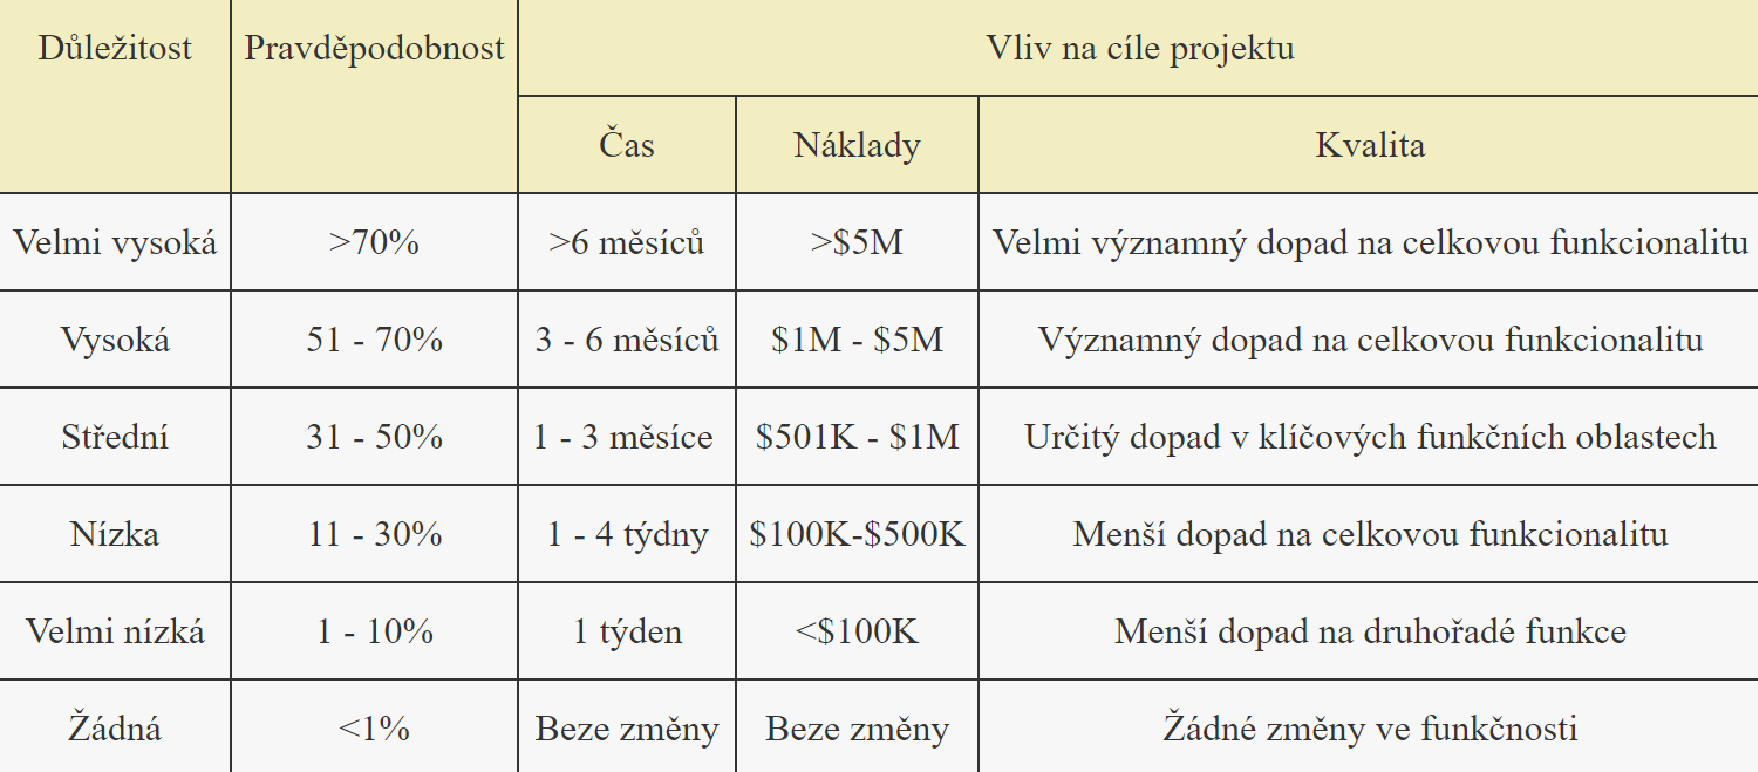
\includegraphics{obrazky-figures/tab2.pdf}}
    \caption{Příklad definic pravděpodobností a jejich důsledků na tři cíle projektu (zdroj inspirováno z~\cite{PMBOK})}
    \label{pravdepodRizik}
    \end{center}
    \end{figure}

    \item \textbf{Matice pravděpodobnosti a dopadu rizika}. Informace se přebírají z~hodnot, které se vytvářely v~předcházejícím bodě, jde prakticky o~jejich grafické zobrazení. Obrázek \ref{maticePravdepodRizik} představuje takovou matici, kdy příležitosti a hrozby jsou zde představeny jako události s~pozitivním či negativním dopadem v~závislosti na výši jejich pravděpodobnosti. Výsledná hodnota v~buňce pak vznikne slovním spojením hodnot na jednotlivých osách a v~případně numerického ohodnocení os pak násobením jejich hodnot (jak je zobrazeno na obrázku \ref{maticePravdepodRizik}). Výsledné skóre pak umožnuje posoudit prioritu s~jakou se musí dané riziko posoudit.
    
    \begin{figure}[ht]
    \begin{center}
    \scalebox{0.55}{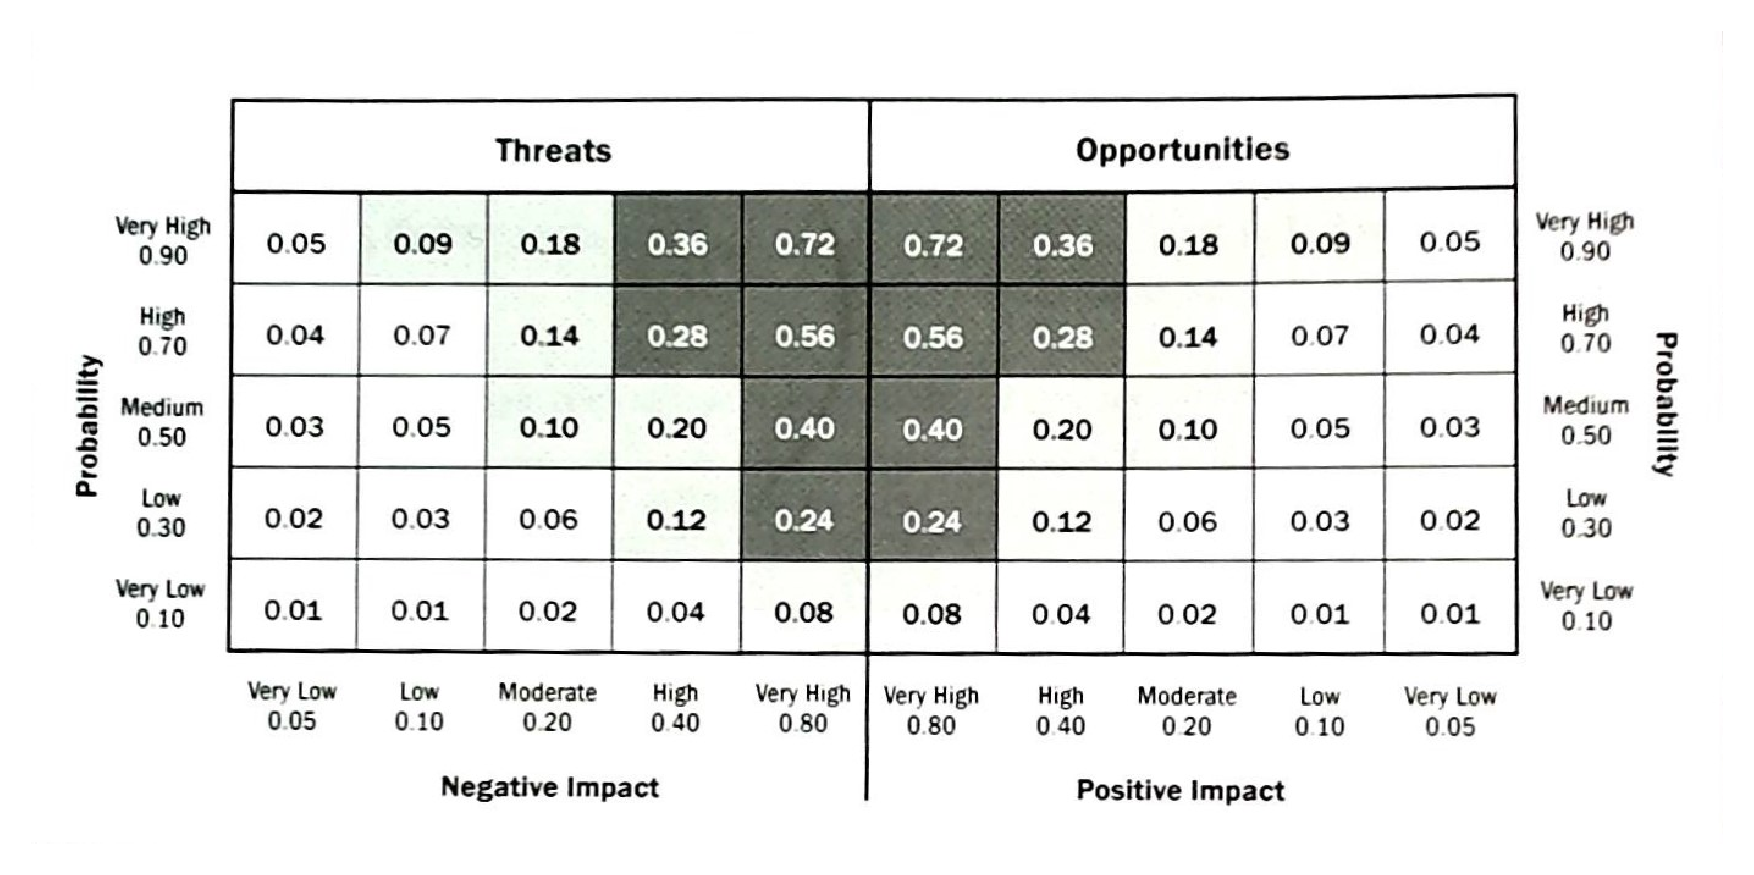
\includegraphics{obrazky-figures/matice.pdf}}
    \caption{Příklad matice pravděpodobnosti a dopadu rizika, která umožňuje posoudit skóre priority u~daných rizik (zdroj převzato z~\cite{PMBOK})}
    \label{maticePravdepodRizik}
    \end{center}
    \end{figure}
    
    \item \textbf{Formát zpráv}. Zde se mají popsat jaký formát budou mít výstupy z~jednotlivých procesů řízení rizik projektu neboli jak se budou dokumentovat, analyzovat či komunikovat mezi členy týmu.
    \item \textbf{Sledování}, způsob, jak se budou dokumentovat rizikové aktivity a jak budou probíhat kontroly jednotlivých procesů.
\end{itemize}

\subsection{Identifikace rizik}
\label{identRizik}

Druhý z~řady procesů řízení rizik projektu je identifikace rizik. Cílem je identifikovat všechna rizika, která nějakým způsobem mohou ovlivnit daný projekt ať už k~pozitivnímu či negativnímu důsledku. K~dobrému pochopení rizik je také potřeba zkoumat jejich zdroje. K~činnostem procesu se může pozvat mnoho účastníku, tj. od projektového manažera, přes experty v~dané oblasti, které se projekt týká, až po koncové uživatele. Je ovšem důležité, aby se identifikace účastnily zainteresované strany, a hlavně členové projektového týmu. Díky tomu pak členové týmu mohou mnohem snadněji rozpoznat a reagovat na rizika. Celý proces se často může opakovat, když s~tím, jak pokračuje životní cyklus projektu, se mohou objevovat nová rizika. Četnost opakování by měla být již určena v~plánu řízení rizik, který je výstupem z~předcházejícího procesu.

Pří zahájení identifikace je potřeba zrevidovat několik vstupních dokument:
\begin{itemize}
    \item \textbf{Plán řízení projektu}, který může obsahovat některé z~následujících komponentů. 
    \begin{itemize}
        \item \textbf{Plán řízení požadavku} může naznačovat cíle náchylné na rizika.
        \item \textbf{Plán řízení časového rozvrhu} naznačuje ne plně pochopené oblasti.
        \item \textbf{Plán řízení nákladů} může obsahovat seznam rizikových oblastí.
        \item \textbf{Plán řízení kvality} naznačuje oblasti s~rizikem nedodržení kvality.
        \item \textbf{Plán řízení zdrojů} může obsahovat informace o~rizikových zdrojích.
        \item \textbf{Plán řízení rizik}, který je výstupem z~předcházejícího procesu, a který může určovat role a zodpovědnosti za rizika, ale také i aktivity a kategorie rizik.
        \item \textbf{Směrný plán rozsahu}, obsahuje strukturu WBS, a také kritéria pro akceptaci výstupů.
        \item \textbf{Směrný plán rozvrhu} má seznam milníku, které se musí dodržet. 
        \item \textbf{Směrný plán nákladu} naznačuje problematické náklady.
         
    \end{itemize}
     \item \textbf{Projektové dokumenty}, mezi kterými můžeme počítat protokol předpokladů, kde jednotlivé předpoklady a omezení můžou ovlivnit důležitost jednotlivých rizik nebo i úroveň celkového rizika projektu. Dále odhady nákladů, odhady časové náročnosti nebo dokumenty správy problémů, kde jednotlivé záznamy mohou zvýšit úroveň rizika. Využít se mohou také registry znalostí nabytých při předcházejících projektech. Ale také dokumentace ze specifikací požadavků, s~požadavky na zdroje a také registr zainteresovaných stran. 
    \item \textbf{Dohody a smlouvy} s~externími dodavateli.
    \item \textbf{Dokumenty obstarávání}, kdy některé zdroje jsou poskytovány externími dodavateli a je potřeba zhodnotit jejich potenciální vlivy na vznik rizik v~projektu.
    \item \textbf{Faktory podnikového prostředí (EEF)}, tím se například myslí přístup k~různým komerčním databázím rizik, nebo k~akademickým a průmyslovým studiím zabývajícími se riziky v~podobných projektech.
    \item \textbf{Procesní aktiva organizace (OPA)}, neboli aktuální informace o~projektu nebo kontrolní seznamy z~předcházejících projektů.
\end{itemize}

Způsob, jakým se jednotlivé dokumenty mají zpracovat a co z~nich pomůže k~identifikací rizik záleží vždy na druhu projektu. Následuje soupiska užitečných technik a nástrojů, které k~tomu mají napomoci.
\begin{itemize}
    \item \textbf{Expertní posudek} se doporučuje podobně jako v~předcházejícím procesu. 
    \item \textbf{Brainstorming}, kde je cílem co nejrychlejší vytvoření seznamu rizik. Děje se to technikou rychlého skoro až bezmyšlenkového navrhování různých rizik. Je doporučeno, aby diskusi vedl moderátor nebo skupina expertů, kteří by udržovali tok diskuse a~zároveň by navrhovali nové kategorie, ve kterých se mohou nacházet rizika. U~brainstormingu je důležité se ujistit, že všechna rizika jsou popsaná správně a srozumitelně.
    \item \textbf{Analýza kontrolních seznamů}. V~těchto seznamech se můžou nacházet informace o~rizicích, které se vyskytovaly na předcházejících projektech, čímž se urychlí identifikace na aktuálním. Doporučuje se ovšem, aby celá identifikace neprobíhala jenom pomocí kontrolních seznamů, když často se tam nenacházejí všechna rizika. Je také vhodné tento seznam jednou za čas aktualizovat o~nové záznamy.
    \item \textbf{Rozhovory} se zkušenějšími členy týmu nebo experty. 
\end{itemize}
 
 Získaná data se pak mohou analyzovat pomocí jedné z~následujících technik.
 
 \begin{itemize}
     \item \textbf{Analýza hlavních příčin}, se používá k~nalézání příčin, které mohou vést ke problémům, následně se pak ze zjištěných dat vytvoří protiopatření. Technika je vhodná i~na hledání příležitostí.
     \item \textbf{Analýza předpokladů a~omezení}, kde cílem je zjistit, zda navržené předpoklady a~omezení jsou validní a zda některé nevedou k~vytvoření negativního nebo i pozitivního rizika.
     \item \textbf{Analýzou dokumentů} lze zjistit hrozby, které se zobrazují jako nekonzistence mezi podobnými dokumenty nebo jako různé nejasnosti. 
     \item \textbf{SWOT analýza}, kde se na projektu zkoumají jeho silné a slabé stránky, ale i~příležitosti a~hrozby (odtud je název techniky, jde o~spojení prvních písmen anglických slov \textit{strengths}, \textit{weaknesses}, \textit{opportunities} a \textit{threats}). Začíná se s~identifikací silných a~slabých stránek firmy, hlavně se zaměřením na projekt (může se ovšem použít i~při analýze společnosti jako takové). Pokračuje se nalezením možných příležitostí vycházejících ze silných stránek a hrozeb vycházejících ze slabých. SWOT analýza také umožňuje určit, zda nějaká silná stránka organizace nekompenzuje hrozby nebo naopak zda nějaká slabá nebrání příležitostem.
 \end{itemize}
 
 Proces identifikace rizik má několik výstupů. Patří mezi ně:
 
 \begin{itemize}
     \item \textbf{Registr rizik} je nejdůležitějším výstupem. Obsahuje soupis všech rizik, pozitivních i~negativních, které se podařilo identifikovat při analýze ze vstupních souborů. Registr je důležitý i při navazujících procesech z~oblasti řízení rizik. Každé riziko by mělo mít své unikátní identifikační číslo a mělo by být srozumitelně popsáno, také by k~němu měla být přiřazena zodpovědná osoba a pokud je to už známo, tak je vhodné uvést i možnou reakci na dané riziko. V~registru se můžou vyskytovat i další dodatečné informace jako například kategorie, aktuální stav, zdroje, možné vlivy na cíle projektu nebo i informace co může způsobit, že se riziko objeví.
     \item \textbf{Zpráva o~rizicích} obsahuje zdroje rizik celkového projektu a také souhrnné informace o~jednotlivých hrozbách. Podobně jako i v~předcházejícím dokumentu i tady se můžou dodat dodatečné informace.
     \item \textbf{Editace projektových dokumentů}. Podle potřeby je vhodné aktualizovat existující projektové dokumenty o~nově zjištěné informace. Týká se to například dokumentu předpokladu, správy problémů či registru znalostí (který následně může pomoci identifikovat rizika na nějakém pozdějším projektu).
 \end{itemize}

\subsection{Kvalitativní analýza rizik}

V~pořadí třetím procesem ve znalostní oblasti řízení rizik je kvalitativní analýza rizik. Jejím cílem je analýza jednotlivých rizik nalezených při identifikaci. Zkoumá se pravděpodobnost jejich vzniku, ale také i jaké můžou mít následky na projekt, priorita, případně i jiné charakteristiky. Tento proces je prováděn po celou dobu trvání projektu. Zároveň se tady pro každé riziko identifikuje zodpovědná osoba, která má na starost naplánovat odpovídající reakci a také má dohlédnout na to, aby firma byla schopna danou reakci uskutečnit.

Vstupem do kvalitativní analýzy rizik je opět několik dokumentů. 
\begin{itemize}
    \item \textbf{Plán řízení projektu}, kde nás hlavně zajímá plán řízení rizik, co všechno tento dokument obsahuje se lze dočíst v~sekci o~Plánování řízení rizik. Pokud tento plán nebyl před tím vytvořen, je možné jej vytvořit na začátku tohoto procesu a před použitím si ho nechat dodatečně odsouhlasit sponzory.
    \item \textbf{Projektové dokumenty}, přesněji se to týká protokolu předpokladů a registru rizik (bližší informace o~těchto dokumentech lze nalézt v~sekci o~identifikaci rizik). Doporučuje se mít také připravený registr zainteresovaných stran, protože někteří z~nich mohou být \uv{vlastníci} nějakého rizika (znamená to, že jejich úkolem je mít připravené protiopatření k~případné hrozbě).
    \item \textbf{Faktory podnikového prostředí (EEF)}
    \item \textbf{Procesní aktiva organizace (OPA)}.
\end{itemize}

Jako v~předcházejících procesech i tady se jako užitečnou techniku či nástroj doporučuje \textbf{expertní posudek}. Použít lze i \textbf{kategorizace rizik}, kdy hrozby a příležitosti jsou rozdělené podle jejich zdrojů nebo podle toho jakou sféru projektu můžou ovlivnit (druhů rozdělení může být i více). Díky kategorizaci pak může projektový tým zaměřovat větší pozornost do míst, o~kterých se ví, že budou nejvíce zatížené riziky.  Co se týče sběru dat, tak tam je vhodné provádět rozhory se zainteresovanými stranami. Při analýze sesbíraných dat se pak můžou použít následující techniky:
\begin{itemize}
    \item \textbf{Hodnocení kvality dat k~rizikům}, sleduje, jak kvalitní jsou data k~jednotlivým rizikům. Pokud by data měla nízkou kvalitu, tak by byl výsledek kvalitativní analýzy nepoužitelný v~daném projektu. Hodnotu dat lze ocenit pomoci dotazníku, který se předloží zainteresovaným stranám a který zjistí jejich chápaní různých charakteristik projektu. 
    \item \textbf{Posouzení pravděpodobnosti a dopadu rizika} zkoumá jaká je pravděpodobnost, že se dané riziko vyskytne. Dále se také ke každému riziku prověřuje jeho možné pozitivní či negativní dopady. Hodnocení rizik lze například provádět pomocí rozhovorů s~účastníky na projektu, přičemž se ale musí brát v~úvahu to, že někteří z~nich můžou mít rozdílné názory na jejich důležitost a tím i pravděpodobnost výskytu a dopady. Možné hodnoty se vybírají z~předem připravené tabulky, která se mohla vytvořit při tvorbě plánu řízení rizik. Možný příklad takové tabulky je na obrázku při definici pravděpodobnosti výskytu rizika a jeho důsledků. Je také doporučené, aby se ke každému riziku přidalo zdůvodnění, proč dostalo dané hodnocení. 
    \item \textbf{Posouzení ostatních parametrů rizik}.Pravděpodobnost výskytu a možné dopady nemusí být jediné charakteristiky, na které se projektový tým může zaměřit. Dále je vhodné zkoumat, jak můžou být hrozby propojené či jak dlouho od výskytu se objeví první vlivy na projektu. Jde například ale i o~to, jak jednoduše může vlastník ovládat výskyt svého rizika případně kontrolovat jeho vlivy na projekt. Dodatečných vlastností může být i mnohem více. Díky nim lze pak mít mnohem lepší představu o~prioritách jednotlivých rizik. 
\end{itemize}
Získaná data je pak vhodné nějakým způsobem graficky prezentovat. Jednou z~technik je \textbf{matice pravděpodobnosti a dopadu}. Jak již název napovídá jde o~grafickou podobu dat z~techniky při analýze dat se stejným jménem. Matice mapuje pravděpodobnost výskytu rizika s~jeho dopady na cíle projektu, díky čemuž je pak lze rozdělit do prioritních skupin (určí se tím, která rizika se musí analyzovat jako první). Hodnoty možného výskytu a vlivů na jeden nebo více cílů v~projektu jsou určeny pomocí tabulky definice pravděpodobnosti a dopadů rizika v~plánu řízení rizik. Je také možné posoudit prioritu rizika pro každý cíl projektu odděleně a výslednou hodnotu určit jako jejich průměr nebo vybrat nejvyšší z~nich. Další grafickou technikou může být \textbf{hierarchický graf}, který se doporučuje, když není možné použít matici a k~porovnání rizik se používají více než jenom dva parametry. Příklad grafu lze vidět na obrázku \ref{hierarKvalita}, kde vliv rizika na projekt je zobrazen jako velikost kroužku. 

    \begin{figure}[ht]
    \begin{center}
    \scalebox{0.5}{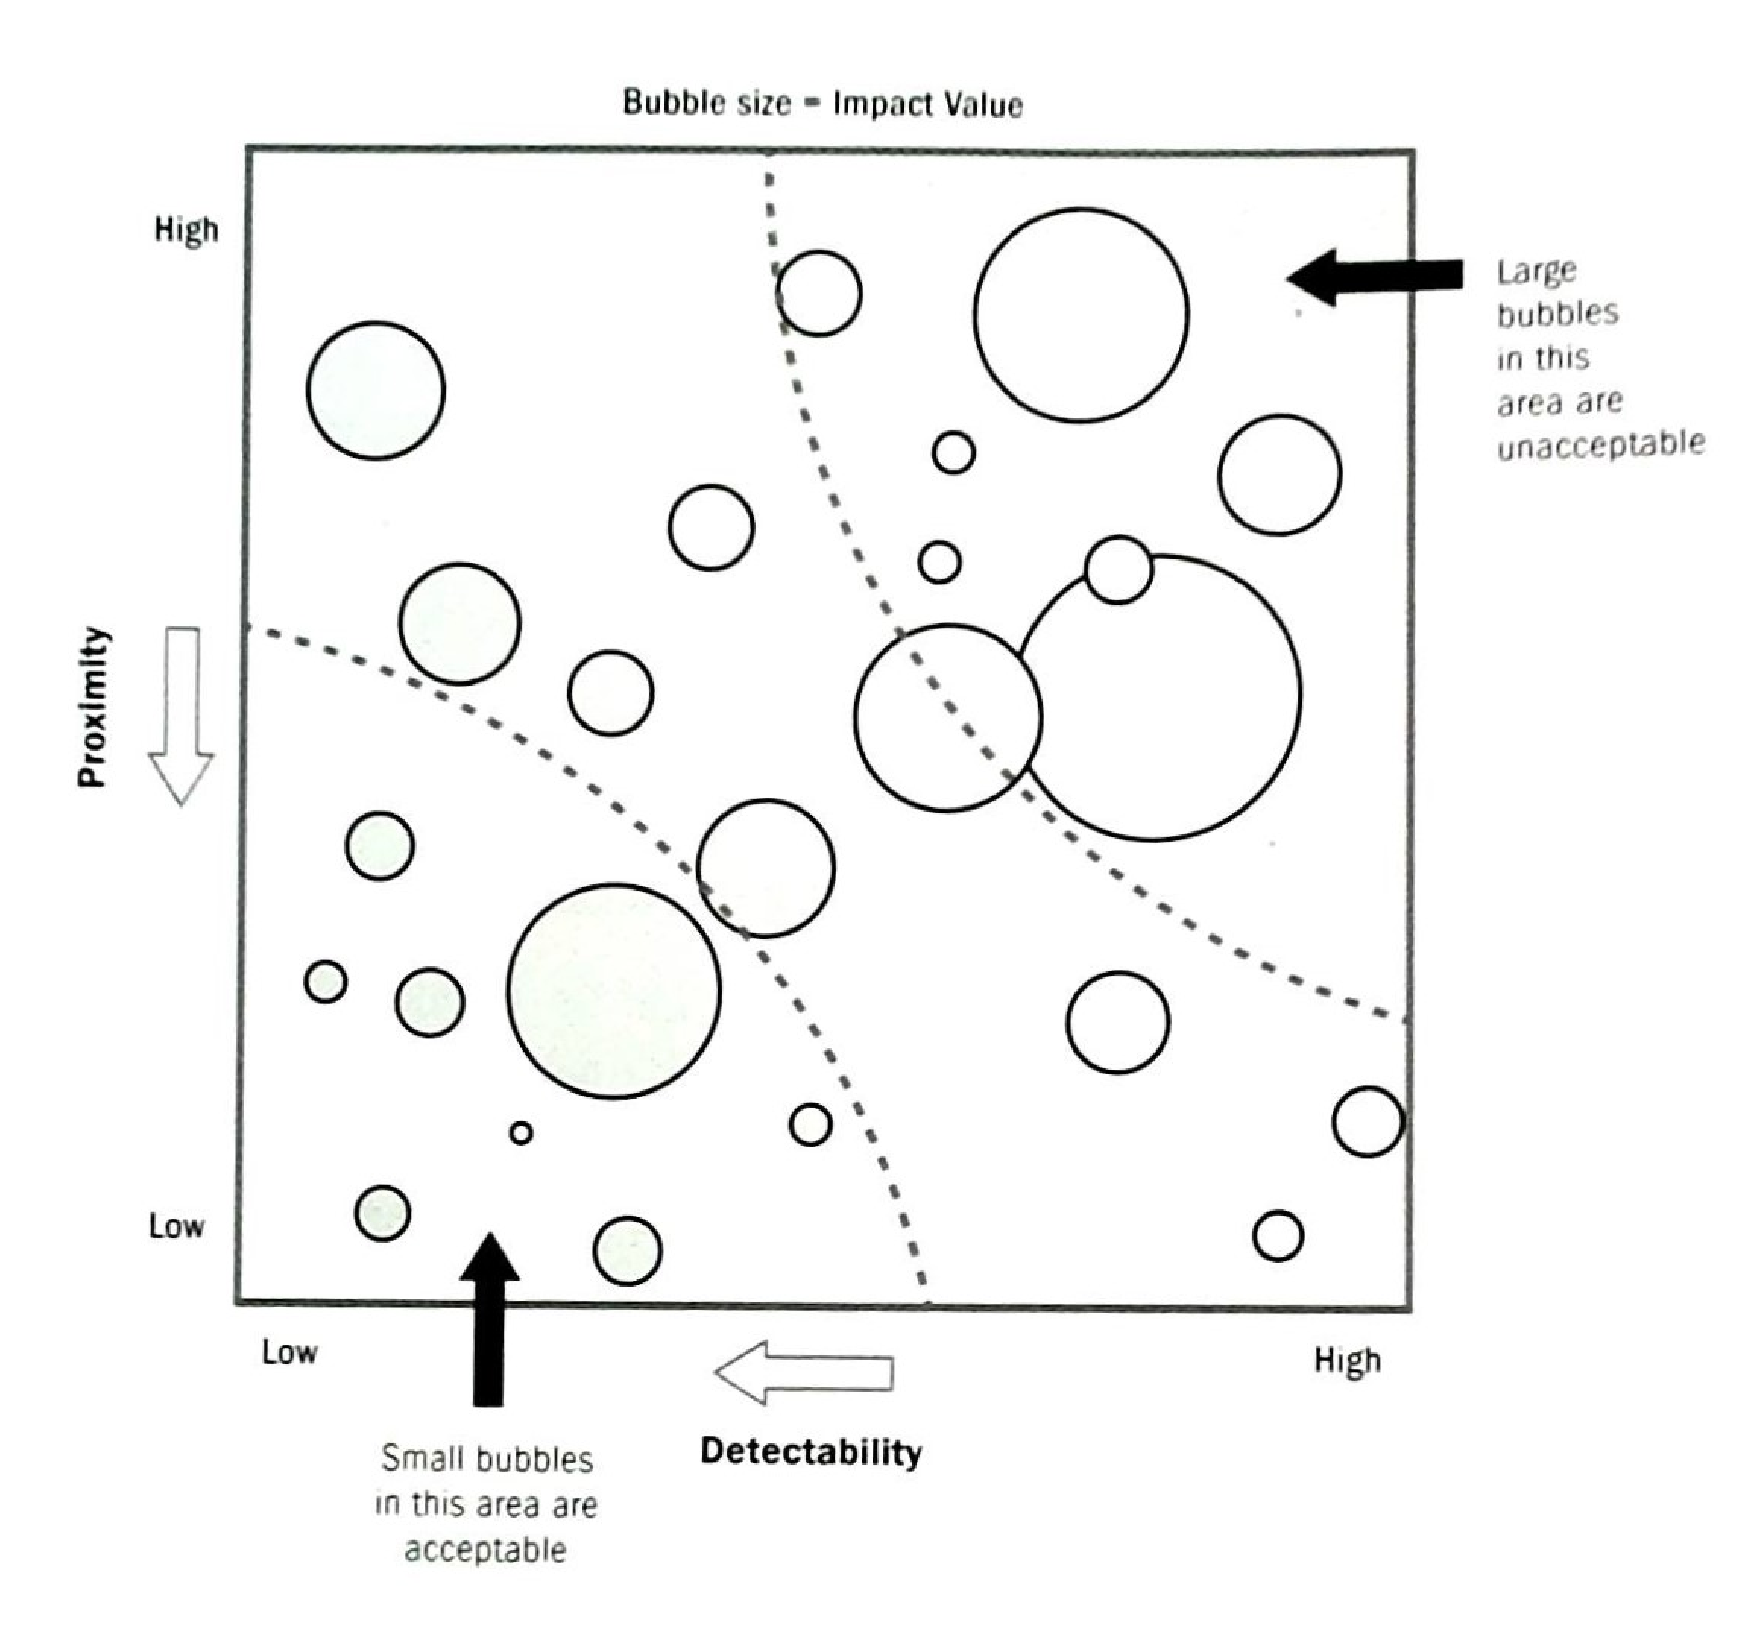
\includegraphics{obrazky-figures/hieGraf.pdf}}
    \caption{Příklad hierarchického grafu, velikost bubliny představuje vliv rizika na projekt (zdroj převzato z~\cite{PMBOK})}
    \label{hierarKvalita}
    \end{center}
    \end{figure}


Při výstupu z~procesu kvalitativní analýzy rizik se podle potřeb \textbf{aktualizují projektové dokumenty}. V~případě, že objevily nové předpoklady, omezení nebo se některý z~nich změnil, tak je nutné nové informace uvést do \textbf{protokolu předpokladů}. Je vhodné také aktualizovat \textbf{dokument správy problémů}. Hlavním výstupem je ale aktualizace \textbf{registru rizik}, kde se přidají nové informace o~prioritách či skóre k~jednotlivým rizikům. Dále se tam můžou přidat informace o~pravděpodobnosti výskytu, možných dopadech, zda je nutné okamžitě riziko řešit, jeho kategorii či oznámení, že riziko se musí ještě více analyzovat. Posledním dokumentem může být \textbf{zpráva o~rizicích}, kde se aktualizují informace o~tom, která rizika jsou nejdůležitější (většinou ty s~největší pravděpodobností vzniku a vlivu na projekt) a také se v~něm vytvoří prioritní rizikový seznam.


\subsection*{Kvantitativní analýza rizik}

Kvantitativní analýza se nemusí provádět na každém projektu, pokud je ovšem v~plánu, tak se provádí po celou dobu běhu projektu a velmi často paralelně s~kvalitativní analýzou.  Často se provádí pouze při velmi rozsáhlých projektech. Cílem procesu je numericky analyzovat jednotlivá rizika a další možné nejasnosti (jejich pravděpodobnost, možné náklady atd.). Výstupy z~toho procesu se velmi hodí do následujícího procesu plánování reakcí.

\subsubsection*{Vstupy}
\begin{itemize}
    \item Plán řízení projektu s~plánem řízení rizik a směrnými plány rozsahu, nákladu a rozvrhu. Směrné plány umožňují určit od jakého bodu se má analýza provádět.
    \item Projektové dokumenty týkajících se rizik, požadavků, nákladů, rozvrhu atd.
    \item EEF
    \item OPA
\end{itemize}
\subsubsection*{Výstupy}
\begin{itemize}
    \item Editace projektových dokumentů, týká se to hlavně zprávy o~rizicích, kde se popisuje celková úroveň rizikovosti projektu, jak vysoké musí být pohotovostní rezervy, seznam a analýza nejzávažnějších rizik, doporučené reakce na rizika atd.
\end{itemize}


\subsection*{Plánování reakcí na rizika}

Tento proces umožňuje definovat, jak reagovat na jednotlivá rizika.  Cílem je minimalizovat hrozby, maximalizovat příležitosti a celkově zmenšit rizikovost projektu. Adekvátní reakce by měly být nákladově efektivní. V~případě potřeby se můžou definovat i náhradní reakce, které se použijí, pokud hlavní bude nedostatčná k~řešení. Kromě reakcí se mohou definovat i strategie rozhodování. V~tomto procesu se také identifikují sekundární rizika, která mohou vzniknou jako následek provádění dané reakce. 

\subsubsection*{Vstupy}
\begin{itemize}
    \item Plán řízení projektu s~plánem řízení rizik a zdrojů (zdroje potřebné pro reakci na rizika) a směrným plánem nákladů.
    \item Projektové dokumenty hlavně zaměřené na rizika, ale také registr zainteresovaných stran nebo dokumenty týkajících se zdrojů.
    \item EEF
    \item OPA
\end{itemize}
\subsubsection*{Výstupy}
\begin{itemize}
    \item Požadavky na změny zaměřené na náklady nebo rozvrh projektu.
    \item Editace plánu řízení, týká se to téměř všech jeho komponent, které se musí upravit, aby bylo možné reakce provést.
    \item Editace projektových dokumentů, kde se hlavně přidají naplánované reakce do registru rizik, ale také se změní data v~dokumentech týkajících se nákladů či rozvrhu.
\end{itemize}


\subsection*{Realizace reakcí na rizika}

Proces, ve kterém se naplánované reakce implementují v~předem dohodnutém pořadí. Vykonává se po celou dobu běhu projektu.

\subsubsection*{Vstupy}
\begin{itemize}
    \item Plán řízení projektu s~plánem řízení rizik identifikují člena týmu, co má na starosti dané riziko.
    \item Projektové dokumenty mezi jinými zprávy a registr rizik.
    \item OPA
\end{itemize}
\subsubsection*{Výstupy}
\begin{itemize}
    \item Požadavky na změny komponent plánu řízení projektu, příkladem můžou být směrný plán rozvrhu a nákladů.
    \item Editace projektových dokumentů např. dokumenty zaměřené na rizika nebo registry získaných znalostí.
\end{itemize}

\subsection*{Sledování rizik} 

V~tomto procesu, který se vykonává po celou dobu prací na projektu, se kontroluje, zda se vykonávají naimplementované reakce, sledují se jednotlivá rizika a zachytávají se a analyzují dříve neznámé hrozby.

\subsubsection*{Vstupy}
\begin{itemize}
    \item Plán řízení projektu s~plánem řízení rizik má zadáno, kdy a jak se kontrola provádí.
    \item Projektové dokumenty zaměřené na rizika.
    \item Údaje o~výkonu práce obsahují informace o~rizicích, které se v~projektu vyskytly.
    \item Zprávy o~výkonu práce, které se provedly.
\end{itemize}
\subsubsection*{Výstupy}
\begin{itemize}
    \item Informace o~výkonu práce představují analyzovaná data o~výkonu, zaměřené na to, jak dobře se projektu daří zvládat jednotlivé výskyty rizik.
    \item Požadavky na změny a opravy, hlavně pak směrných plánů nákladů a rozvrhu.
    \item Editace plánu řízení projektu dle potřeby.
    \item Editace projektových dokumentů rizik nebo různých předpokladů.
    \item Editace OPA o~různé šablony z~oblasti řízení rizik.
\end{itemize}

\section{Řízení obstarávání v~rámci projektu}
\label{RizeniObstaravani}

V~této znalostní oblasti se řídí výběr a nákup potřebných zdrojů od externích dodavatelů. Celkově se oblast hlavně zabývá uzavíráním potřebných dohod a smluv. Ačkoliv je manažer projektu většinou ten, který vyjednává jednotlivé zdroje, tak zpravidla nemá potřebné vzdělání či pravomoci k~tomu, aby smlouvu podepsal a tím zavázal svou organizaci v~plnění dané úmluvy. V~oblasti se nacházejí tři následující procesy.

\subsection*{Plánování řízení obstarávání}

Cílem procesu je rozhodnou a naplánovat co bude nutné obstarat z~externích zdrojů pro potřeby projektu. Zároveň se také určuje způsob, místo a čas, kdy se bude produkt muset získat. 

\subsubsection*{Vstupy}
\begin{itemize}
    \item Zákládající listina projektu obsahuje popis projektu a předem dohodnuté financování zdrojů.
    \item Obchodní dokumenty s~projektovým záměrem a plánem řízení přínosů.
    \item Plán řízení projektu s~komponentami zaměřenými na rozsah, kvalitu a zdroje.
    \item Projektové dokumenty s~požadavky na zdroje a celkovými požadavky na projekt.
    \item EEF
    \item OPA
\end{itemize}
\subsubsection*{Výstupy}
\begin{itemize}
    \item Plán řízení obstarávání obsahuje seznam aktivit, co v~průběhu provádění procesů řízení obstarávaní budou provádět. Dále může obsahovat návody, jak řídit kontrakty a jejich právní normy, seznam preferovaných externích dodavatelů atd. 
    \item Strategie obstarávání určují, jakým způsobem se produkt doručí a jak se za něho bude platit.
    \item Cenové nabídky jsou dokumenty na základě kterých lze porovnat nabídky různých externích dodavatelů.
    \item Prohlášení o~práci pro každou zakázku určuje co má daný produkt umožňovat.
    \item Výběrová kritéria zdrojů, používá se, aby se vybral ten nevhodnější dodavatel.
    \item Rozhodnutí, zda vyrobit nebo koupit produkt se provádí pomocí analýzy, zda je samotný projektový tým schopen produkt dodat nebo se musí získat zvenčí.
    \item Nezávislé odhady ceny pro rozsáhlejší produkty. Může být zadáno externí firmě.
    \item Požadavky na změny týkajících se obstarávaní produktů.
    \item Editace projektových dokumentů, které se hlavně týkají požadavků nebo možných rizik.
    \item Editace OPA s~informacemi o~kvalitních externích dodavatelích.
\end{itemize}

\subsection*{Řízení obstarávání}

V~tomto procesu se vyhodnocují nabídky od potenciálních dodavatelů. Následuje pak vybrání nejlepší nabídky a sepsání dohody s~daným dodavatelem. Proces se periodicky opakuje.

\subsubsection*{Vstupy}
\begin{itemize}
    \item Plán řízení projektu, který mezi jinými obsahuje také plány řízení zaměřené na získávání zdrojů a možných rizik z~toho plynoucích.
    \item Projektové dokumenty jako registr znalostí, rizik, nebo dokumenty týkajících se rozvrhu projektu či dokumenty popisující požadavky na produkty co se mají dodat.
    \item Dokumenty obstarávání, které mohou pomoci k~vybrání vyhovujícího dodavatele.
    \item Nabídky dodavatelů určující, co jejich produkt je schopen provést.
    \item EEF
    \item OPA
\end{itemize}
\subsubsection*{Výstupy}
\begin{itemize}
    \item Vybraní dodavatelé, kteří nejlépe splňují požadovaná kritéria.
    \item Dohody a smlouvy s~dodavateli, dokumentují způsoby dodání produktu, platby, podmínky atd.
    \item Požadavky na změny, které vzešly na základě procesu.
    \item Editace plánu řízení projektu a jeho komponent, informace vycházející z~tohoto procesu.
    \item Editace projektových dokumentu týkajících se hlavě požadavků, zdrojů, rizik a zainteresovaných stran.
    \item Editace OPA, kde se můžou přidat informace a zkušenosti s~důvěryhodnými podavateli.
\end{itemize}


\subsection*{Kontrola obstarávání}

Poslední proces této znalostní oblasti, ve kterém se monitorují, jak se dodržují dohodnuté kontrakty. Dále se zde také navrhují požadované změny a zodpovídá i za uzavření celé dohody. Proces se provádí kdykoliv to projekt vyžaduje.

\subsubsection*{Vstupy}
\begin{itemize}
    \item Plán řízení projektu s~plány na řízení požadavků, obstarávání, změn a rizik.
    \item Projektové dokumenty zaměřené na požadavky, rizika, kvalitu a podobně.
    \item Dohody a smlouvy s~externími dodavateli produktů.
    \item Dokumenty obstarávání poskytují dodatečné informace k~obstarávání.
    \item Schválené požadavky na změny podmínek v~dohodách.
    \item Údaje o~výkonu práce. 
    \item EEF
    \item OPA
\end{itemize}
\subsubsection*{Výstupy}
\begin{itemize}
    \item Uzavřené dodávky, kde se dodavateli oznámí, že kontrakt byl naplněn a provádí se jeho dokončení.
    \item Informace o~výkonu práce. 
    \item Editace dokumentů obstarávání o~dodateční informace\,--\,schválené/neschválené změny atd.
    \item Požadavky na změny v~projektu.
    \item Editace plánu projektu a jeho komponent k~řízení rizik, řízení obstarávání a dále směrné plány rozvrhu a nákladů.
    \item Editace projektových dokumentů, hlavně pak dokumenty týkající se požadavků.
    \item Editace OPA s~informacemi o~rozvrhu plateb, s~hodnocením dodavatelů atd.
\end{itemize}


\section{Řízení zainteresovaných stran}
\label{RizeniZainterStran}

Poslední znalostní oblast. Jejím cílem je určit všechny \textbf{zainteresované strany} (neboli všechny subjekty, které mohou mít vliv na projekt nebo být nějakým způsobem projektem ovlivněni). Dále se analyzují jejich očekávaní od projektu, míru vlivu a tvoří se strategie, jak s~nimi jednat a jak je začlenit do vývoje na projektu. Zajištění spokojenosti zainteresovaných stran by se měla považovat jako jeden z~nejdůležitějších cílů projektu. V~oblasti se nacházejí čtyři procesy.


\subsection*{Identifikace zainteresovaných stran}

Jak již název napovídá v~tomto procesu se identifikují všechny zainteresované strany. Zároveň se také analyzují jejich vlivy, zájmy a požadavky na projektu. Proces se periodicky opakuje a umožňuje projektovému týmu vybrat správné způsoby, jak zainteresované strany zapojit do procesu řízení projektu.


\subsubsection*{Vstupy}
\begin{itemize}
    \item Zákládající listina projektu obsahuje seznam nejdůležitějších zainteresovaných stran. 
    \item Obchodní dokumenty, hlavně pak dokumenty projektového zájmu a plánu řízení přínosu mohou obsahovat informace o~zainteresovaných stranách. 
    \item Plán řízení projektu nemusí být při první identifikaci ještě zcela dokončen. V~pozdějších fázích projektu, ale komponenty plánu řízení komunikace a plánu zapojení zainteresovaných stran, mohou pomoci v~tomto procesu.
    \item Projektové dokumenty se využijí až v~pozdějších fázích projektu, hlavně pak dokumenty správy změn, problémů nebo i dokumenty požadavků.
    \item Dohody a smlouvy týkající se projektu.
    \item EEF
    \item OPA
\end{itemize}
\subsubsection*{Výstupy}
\begin{itemize}
    \item Registr zainteresovaných stran může obsahovat jejich identifikaci, hodnocení či klasifikaci.
    \item Požadavky na změny, které vyplynuly z~nově identifikovaných zainteresovaných stran.
    \item Editace plánu řízení, kde v~pozdějších iteracích se mohou přidat, či změnit informace v~plánech řízení komunikace, rizik, požadavků nebo plánu zapojení zainteresovaných stran.
    \item Editace projektových dokumentů rizik, předpokladů nebo problémů.
\end{itemize}


\subsection*{Plánování zapojení zainteresovaných stran}

V~tomto procesu je cílem zkoumat požadavky jednotlivých zainteresovaných stran. Dále se také analyzují jejich zájmy, vlivy a očekávaní na projektu. To vše se pak použije k~tomu, aby se vytvořila odpovídající strategie k~zapojení zainteresovaných stran k~činnostem na projektu. 

\subsubsection*{Vstupy}
\begin{itemize}
    \item Zakládající listina projektu obsahuje informace o~projektu.
    \item Plán řízeni projektu s~plány řízení rizik, zdrojů a komunikace. 
    \item Projektové dokumenty s~registry rizik, zainteresovaných stran, s~dokumenty o~předpokladech, problémech či změnách, použít by se měl i rozvrh projektu.
    \item Dohody a smlouvy se zainteresovanými stranami.
    \item EEF
    \item OPA
\end{itemize}
\subsubsection*{Výstupy}
\begin{itemize}
    \item Plán zapojení zainteresovaných stran, ve kterém se popisují strategie a aktivity potřebné k~co nejlepšímu zapojení daného subjektu v~projektu.
\end{itemize}



\subsection*{Řízení zapojení zainteresovaných stran}

Další z~procesu co se provádějí po celou dobu pracovních aktivit na projektu. V~jeho průběhu se komunikuje se zainteresovanými stranami a ve spolupráci s~nimi se řeší problémy na projektu. Tím se lze ujistit, že zainteresované strany jsou vždy plně informované o~stavu projektu.

\subsubsection*{Vstupy}
\begin{itemize}
    \item Plán řízení projektu s~komponentami zaměřenými na rizika, komunikaci, zainteresované strany a změny.
    \item Projektové dokumenty s~registry znalostí a zainteresovaných stran nebo dokumenty správy změn a problémů.
    \item EEF
    \item OPA
\end{itemize}
\subsubsection*{Výstupy}
\begin{itemize}
    \item Požadavky na změny, které vzešly ze spolupráce se zainteresovanými stranami.
    \item Editace plánu řízení projektu pro lepší řízení komunikace a zapojení zainteresovaných stran.
    \item Editace projektových dokumentů, které se mohly využít i při vstupu.
\end{itemize}


\subsection*{Monitorování zapojení zainteresovaných stran}

V~posledním procesu oblasti řízení zainteresovaných stran se monitoruje jejich vztah s~projektem a v~případě potřeby se upravují strategie používané k~podpoře jejich zapojení. Proces patří do skupiny těch, které se uskutečňují po celou dobu životního cyklu projektu.

\subsubsection*{Vstupy}
\begin{itemize}
    \item Plán řízení projektu a plány řízení zdrojů, komunikace a zainteresovaných stran.
    \item Projektové dokumenty zaměřené na rizika, zainteresované strany a komunikaci.
    \item Údaje o~výkonu práce a stupni zapojení zainteresovaných stran.
    \item EEF
    \item OPA
\end{itemize}
\subsubsection*{Výstupy}
\begin{itemize}
    \item Informace o~výkonu práce shrnují záznamy z~dokumentu údajů o~výkonu práce.
    \item Požadavky na změny zapojení zainteresovaných stran.
    \item Editace plánu řízení projektu týkajících se zdrojů, komunikace a zainteresovaných stran.
    \item Editace projektových dokumentů, hlavně pak registry rizik, zainteresovaných stran a~znalostí.
\end{itemize}

\chapter{Agilní řízení projektů}
\label{agilni}

Jedním z~problémů klasického řízení projektu jsou jeho reakce na změny v~pozdějších fázích projektu. U~tohoto typu řízení se často stává, že zákazník vidí až výsledný produkt a ten nemusí být podle jeho představ, následují pak vynucené změny a hrozí prodlení v~nasazení produktu s~možným překročením dohodnutého rozpočtu. Dalším problémem může být i to, že se nejdříve tvoří různé plány a návrhy, ale výsledný produkt se tvoří a dodává až později. Všechny tyto problémy se snaží řešit různé agilní metodiky. Pokud není určeno jinak, tak informace jsou převzaté z~knihy \textit{Agile Practice Guide}, která je také od firmy \textbf{PMI} \cite{PMBOKAgile}.

Agilní řízení projektů umožňuje pracovat a úspěšně dokončit projekty, které jsou charakteristické svou nejasností vycházející ze změn v~požadavcích. Díky tomu lze také lépe reagovat na změny a tím i na nově se vyskytující rizika.

Agilní životní cyklus je kombinací iterativního, kde se vytvářejí prototypy, které se prezentují zainteresovaným stranám k~posouzení, získané informace se použijí v~dalších iteracích, a inkrementálního životního cyklu, kde se zákazníkovi v~pravidelných cyklech dodávají jednotlivé části výsledného produktu. Díky tomuto přístupu se lze dříve odhalit nedorozumění v~požadavcích.  Příklad agilního řízení projektu v~porovnání s~vodopádovým modelem lze vidět na obrázku \ref{agilniVyvoj}.

    \begin{figure}[ht]
    \begin{center}
    \scalebox{0.5}{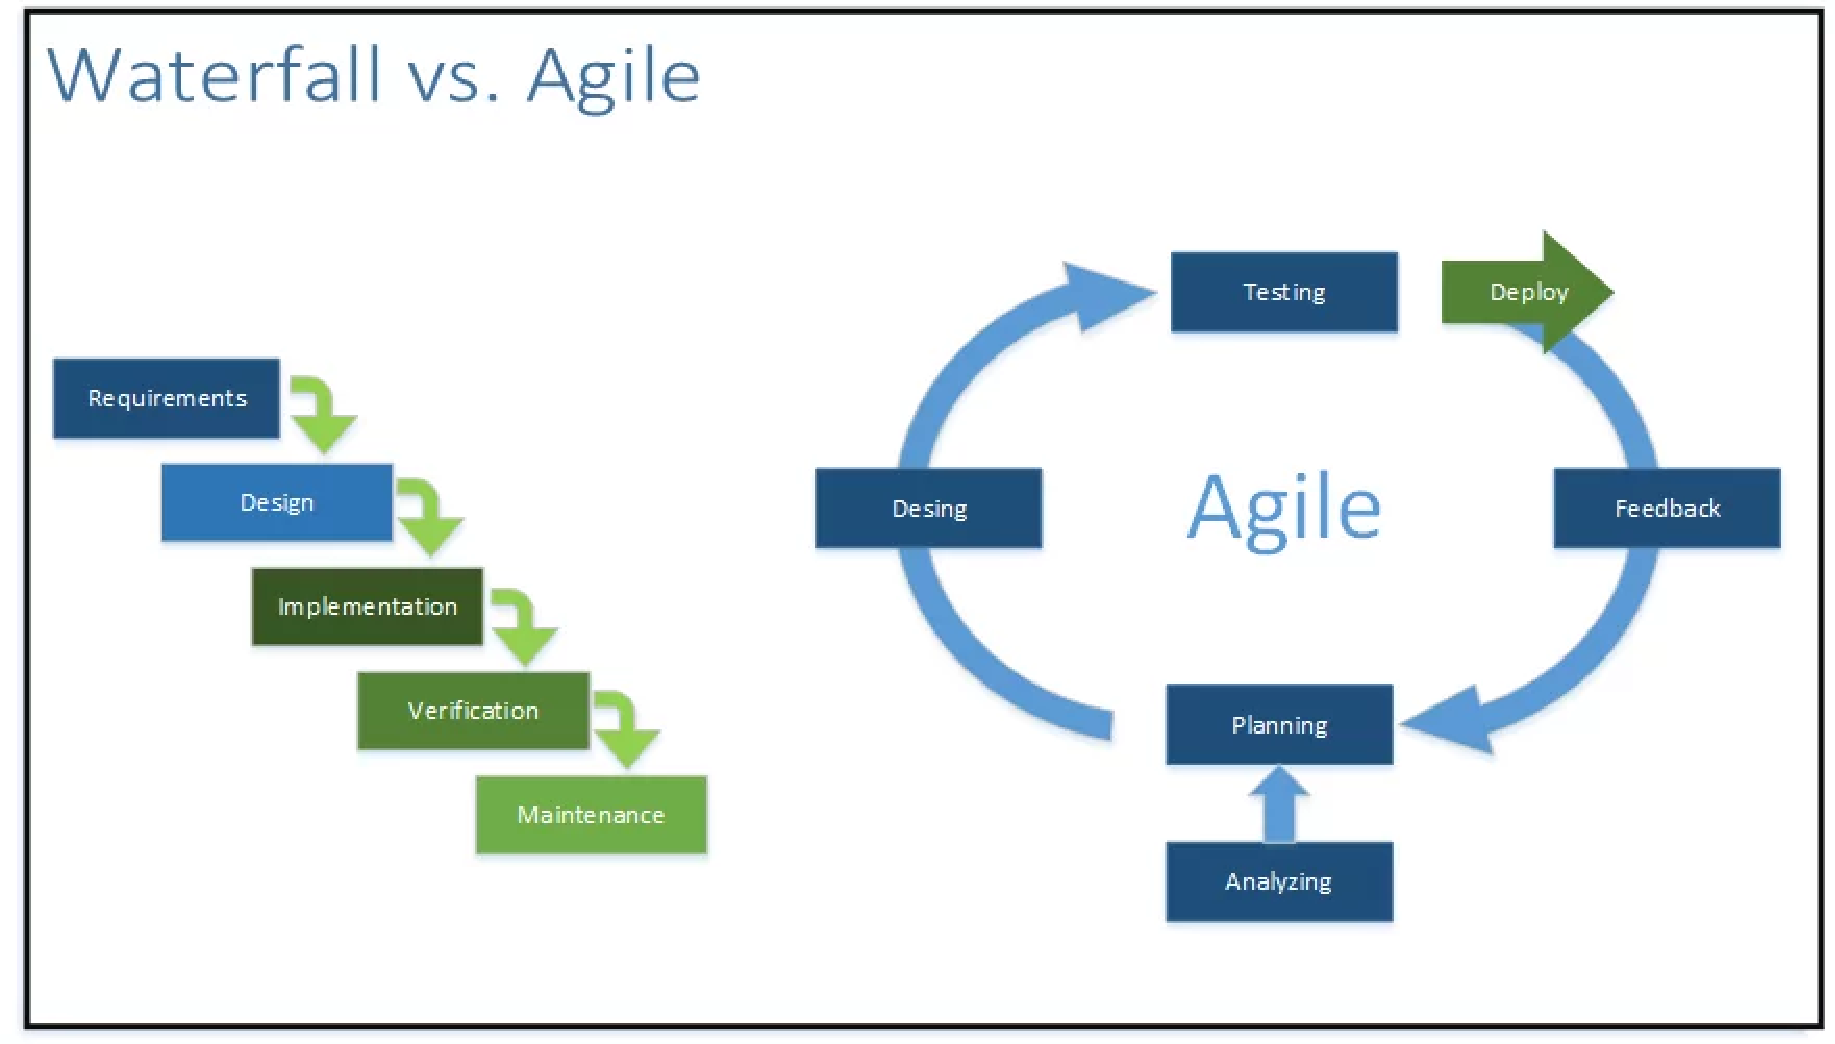
\includegraphics{obrazky-figures/waterfallAgile.pdf}}
    \caption{Možný agilní vývoj v~porovnání s~klasickým vodopádovým modelem (zdroj převzato z~\cite{agileObraz})}
    \label{agilniVyvoj}
    \end{center}
    \end{figure}

\section{Agilní přístup ke znalostním oblastem}
Znalostní oblasti, které lze využívat v~klasickém řízení projektu, lze také v~pozměněné formě využívat i v~agilním řízení. 

\begin{itemize}
    \item \textbf{Řízení integrace projektu} je podobné jako v~klasickém řízení. Jak bylo psáno v~části \ref{RizeniIntegrace}, hlavním účastníkem je manažer projektu. Agilní řízení se v~této znalostní oblasti více zaměřuje na zapojení členů týmu, kdy je jím přidělena větší zodpovědnost k~plánování a dodávání výsledků. Úkolem manažera projektu je pak vytvořit odpovídající podmínky pro členy týmu a připravit je na lepší zvládání změn.
    \item \textbf{Řízení rozsahu prací projektu}. Agilní řízení projektu uznává, a dokonce i vítá skutečnost, že požadavky v~projektu nejsou od začátku úplně známé a že se v~průběhu řešení můžou měnit. To způsobuje, že při počátečním plánování nelze plně určit celkový rozsah projektu. Z~toho důvodu se klade důraz na naplánování procesů, které se budou v~průběhu projektu opakovat, jejichž cílem je postupně stanovit celkový rozsah aktivit na projektu.
    \item \textbf{Řízení časového plánu v~rámci projektu}. Jak bylo již dříve zmíněno i v~klasickém řízení projektu se používají jisté agilní metody k~řízení časového plánu. U~menších projektů a firem se osvědčilo provádění relativně krátkých cyklu, ve kterých se pracuje na části projektu. Na konci cyklu se pak zhodnotí dosavadní výsledky a v~případě potřeby se přizpůsobí další cykly. Rozsáhlejší projekty a organizace, ale vyžadují alespoň částečné dlouhodobé časové plány (např. pro potřeby přerozdělení zdrojů). Pro ně se pak můžou použít hybridní metody spojující agilní a klasický přístup. 
    \item \textbf{Řízení nákladů projektu} může být problematické, pokud ještě není znám celkový rozsah aktivit v~projektu. Z~důvodu těchto nejasností není možné vytvořit detailní plán celkových nákladů. Místo toho se vytvářejí nedetailní dlouhodobé plány, které představují pravděpodobné náklady a které lze kdykoliv přizpůsobit. Pokud jsou detailní plány nákladu potřeba, tak se vytvářejí pouze pro krátké časové úseky.
    \item \textbf{Řízení kvality v~rámci projektu}. Jelikož se v~agilním řízení projektu doručují jednotlivé částí (iterace) produktu postupně, tak je možné již během vývoje kontrolovat kvalitu výsledků a tím lépe (a za méně nákladů) napravit případné nedostatky. Aby se kvalita práce na projektu udržela na konsistentní úrovni (případně i zlepšila), tak se periodicky kontroluje efektivita procesů týkajících se kvality. V~případě, že se zjistí nedostatky, tak se uvažuje o~změně či úplném vynechání procesu.
    \item \textbf{Řízení zdrojů v~rámci projektu}. Projekty mívají často vysokou úroveň nejasností, může být proto problematické naplánovat, kdy a jaké zdroje (ať už fyzické nebo lidské) budou potřeba. Z~tohoto důvodu je proto vhodné mít dohody a smlouvy s~dodavateli, kteří jsou schopni velmi rychle potřebné zdroje zajistit. Je důležité se také zaměřit na lidské zdroje projektu\,--\,členy týmu. Dle agilních principů mají na projektu pracovat efektivní, nejlépe samo se řídící týmy. Tyto spolupracující týmu, pak mají být základem k~úspěšnému dokončení projektu.
    \item \textbf{Řízení komunikace v~rámci projektu}. Jelikož agilní vývoj mnohem častěji vítá změny, tak se komunikace, ať už mezi členy týmu anebo se zainteresovanými stranami, stává jednou z~nejdůležitějších složek agilního řízení projektu. Členové týmu by vždy měli mít svobodný přístup ke všem potřebným informacím a mělo by jim být umožněno se fyzicky účastnit týmových meetingů (tzv. kolokace členů týmu). Dále je také nutné více spolupracovat se zainteresovanými stranami.  
    \item \textbf{Řízení rizik projektu}. Rozdělení projektu na menší části umožňuje posuzovat rizika v~mnohem menším měřítku. Díky tomu se pak nemusí vytvářet zdlouhavé, dopředné identifikace a analýzy rizik celého projektu. Rizika se berou v~úvahu již při výběru části projektu. V~případě, že tým ví, že se jistá hrozba, na kterou není připraven, může v~dané části vyskytnou, tak si vždy může vybrat jiný úsek projektu. Při tvorbě dané části se pak rizika identifikují, analyzují a v~případě výskytu i řídí. Již hotové části projektu se pak ještě dodatečně opakovaně analyzují. Podporuje se také sdílení vědomostí a znalostí o~rizicích mezi jednotlivými týmy. Rozdělení na části a jejich postupné doručování zákazníku umožňuje snížit riziko nedodržení kvality projektu, kterou zákazník požaduje. Problematickým rizikem v~agilním řízení může být nedodržení rozpočtu, když, jak se již zmínilo v~této kapitole v~řízení nákladů projektu, neexistuje dopředný podrobný plán celkových nákladů
    \item \textbf{Řízení obstarávání v~rámci projektu}. V~menších projektech může být vhodné navázat bližší spolupráci s~dodavatelem produktu, případně ho začlenit do projektového týmu. Díky tomuto přístupu dodavatel i příjemce (v~tomto případě firma co projekt řeší) sdílí rizika i výhody na projektu a mají větší motivaci ho úspěšně dokončit. U~větších projektů může být potřeba použít kombinovaný přístup, když pro část zdrojů se použije adaptivní přístup a pro další klasický stabilní. Tuto kombinaci je ale nutné si zajistit smlouvou, kdy se adaptivní část může vyjednat v~dodatcích k~dohodě.
    \item \textbf{Řízení zainteresovaných stran}. Z~důvodu toho, jak se projekty provádějí v~agilním řízení, tak je zapojení zainteresovaných stran v~mnohem větší míře než u~klasického řízení. Často se pak stává, že členové týmu přímo komunikují se zainteresovanými stranami, aby od nich zjistili potřebnou zpětnou vazbu či podrobnosti k~požadavkům. Díky tomuto přístupu se zmenšují rizika nespokojenosti zainteresovaných stran a zvětšuje pravděpodobnost úspěšného dokončení projektu. 
\end{itemize}


\chapter{Návrh nástroje pro podporu řízení rizik}
\label{navrh}

Tato kapitola popisuje návrh nástroje pro řízení rizik. V~první části je popsána specifikace požadavků na daný nástroj. Následuje pak návrh aplikace s~use-case diagramem, schématem struktury databáze a návrhem několika obrazovek uživatelského rozhraní. Při popisu návrhu databáze se používá zkratka \textbf{CRUD}, jedná se o~spojení anglických slov \textit{create}, \textit{read}, \textit{update} a \textit{delete}, představující základní operace nad daty v~databázi. Do češtiny lze tyto slova přeložit jako \textbf{vytvořit}, \textbf{číst}, \textbf{editovat} a \textbf{smazat}.

\section{Specifikace požadavků}

V~posledních letech se webové aplikace staly velice oblíbenou technologií. Je to způsobeno čím dál tím rychlejším internetovým připojením, ale také rozsáhlou kompatibilitou s~různými operačními systémy, které běží na často velmi rozdílných zařízeních. Z~tohoto důvodu by výsledný nástroj měl být webovou aplikací. 

Zaměření aplikace by mělo být na plánování řízení, identifikaci a kvalitativní analýzu rizik. Nástroj by měl umožňovat zobrazovat a upravovat registr rizik, ve kterém lze vyhledávat. Dle \ref{identRizik} lze pomocí dotazníku identifikovat a analyzovat rizika na projektu, bude proto vhodné tyto dotazníky a jejich otázky v~aplikaci vytvářet a uchovávat. Jedna otázka se může vyskytovat ve vícero dotaznících. K~identifikaci rizik lze použít i SWOT analýza jejímž výstupem je SWOT tabulka, aplikace by proto měla umožňovat její vytvoření. Uživatelům by mělo být také dovoleno zobrazovat rizika v~matici pravděpodobnosti a~dopadů. 

Co se týče uživatelů, tak těm by mělo být dovoleno se přihlašovat a odhlašovat, přičemž aplikace by si měla přihlášení na daném počítači pamatovat a v~případě neaktivity uživatele by po jisté době mělo dojít k~automatickému odhlášení. Mělo by existovat více uživatelských rolí, přičemž obyčejnému uživateli by mělo být dovoleno zobrazovat pouze projekty, ke kterým je přihlášen. Manažeru projektu by nástroj měl umožňovat spravovat své projekty, dále i přiřazovat a odhlašovat řešitele projektu. Ke každému řešiteli by mělo být možné přidat rizika, která má na starosti.
Výsledná aplikace by měla být jednoduchá na používání s~moderním a responzivním designem.

\section{Diagram případů užití}

Na základě specifikace požadavků byl navrhnut diagram případu užití, který je k~vidění na obrázku \ref{usecase}. V~systému se budou nacházet tři role: \textbf{člen týmu řešitelů}, \textbf{projektový manažér} (může být také manažerem řízení rizik) a \textbf{projektový administrátor}. Role jsou propojené tak, aby role s~největšími pravomocmi mohly provádět i činnosti rolí s~nižším oprávněním neboli administrátor může provádět případy užití člena týmu.

    \begin{figure}[!htbp]
    \begin{center}
    \scalebox{0.75}{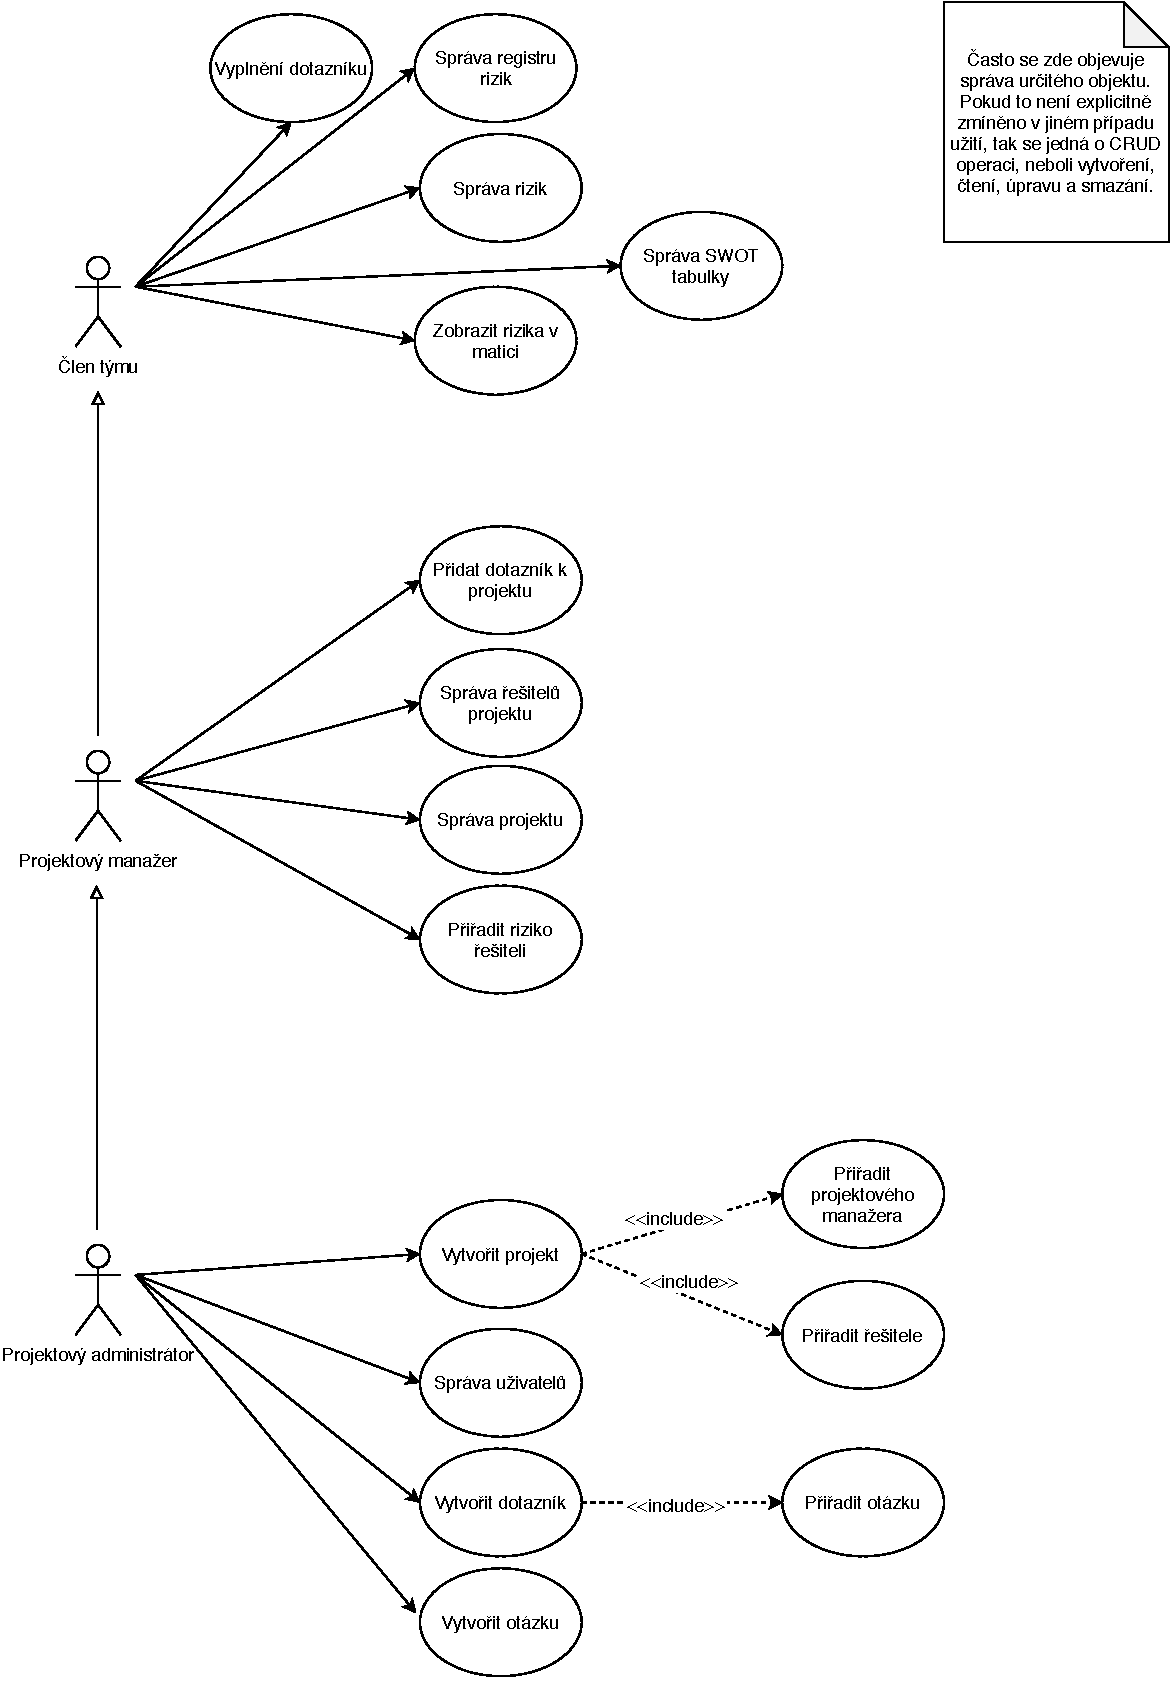
\includegraphics{obrazky-figures/useCase2.pdf}}
    \caption{Diagram případů užití [zdroj vlastní]}
    \label{usecase}
    \end{center}
    \end{figure}
    
\subsection*{Projektový administrátor}

Je to uživatel systému, který má na starost administrativní úkony na projektu. Jedná se tedy o~tyto případy užití: 

\begin{itemize}
    \item \textbf{Vytvořit projekt}, ve kterém se založí projekt, přidají se mu potřebné atributy a~zároveň se k~němu také přiřadí jeho manažer a ostatní členové řešitelského týmu.
    \item \textbf{Správa uživatelů}, obsahuje všechny činnosti nad účty všech uživatelů (jak se zmiňuje v~poznámce, jedná se o~CRUD akce).
    \item \textbf{Vytvořit dotazník}, v~tomto užití bude projektový administrátor tvořit dotazníky z~předem vytvořených otázek. 
    \item \textbf{Vytvořit otázku}, kde se vytvoří otázka a zároveň se i vyberou i možné odpovědi. Jedna otázka se pak bude moct vyskytovat ve více dotaznících. 
\end{itemize}

\subsection*{Projektový manažer}

Může se také označovat jako manažer řízení rizik nebo manažer rizik. V~jeho kompetencích je řízení projektu a členů, kteří na něm pracují. Může přistupovat pouze k~projektům, ke kterým je přiřazen.

\begin{itemize}
    \item \textbf{Přidat dotazník k~projektu}, kde se předem vytvořený dotazník může přiřadit k~projektu. Jeden dotazník se může využít i v~jiných projektech.  
    \item \textbf{Správa řešitelů projektu}, zpřístupní funkce díky, kterým bude manažer schopen členy týmu ze svého projektu odhlašovat či přihlašovat nové řešitelé.
    \item \textbf{Správa projektu}, umožní celkovou správu všech atributů projektu.
    \item \textbf{Přiřadit riziko řešiteli}, se použije, když manažer dá nějakému členu řešitelského týmu za úkol správu daného rizika na projektu (neboli dá za úkol toto riziko plně identifikovat a analyzovat).
\end{itemize}

\subsection*{Člen týmu}

Představuje klasického řádového člena řešitelského týmu. Tato role má v~nástroji nejméně oprávnění. Jsou mu přiřazené následující případy užití: 

\begin{itemize}
    \item \textbf{Vyplnění dotazníku}, kde člen týmu bude moct odpovědět na dotazník týkající se projektu, ke kterému je přiřazen.
    \item \textbf{Správa registru rizik} rizik umožní vyhledávat a filtrovat výsledky centrálním registru rizik dané společnosti.
    \item \textbf{Správa rizik}, v~tomto případu užití bude moct člen týmu vykonávat celkovou správu rizik na daném projektu.
    \item \textbf{Správa SWOT tabulky}, kde člen týmu (ale také i také i ostatní role s~většími právy) budou moci vytvářet, číst, upravovat či mazat SWOT tabulky, které obsahují výstup ze SWOT analýzy.
    \item \textbf{Zobrazit rizika v~matici}, jde o~grafickou prezentaci rizik v~matici pravděpodobností a dopadů. Hodnoty pravděpodobnosti výskytu a dopadu rizika se získají z~jeho atributů.
\end{itemize}

\section{Schéma databáze}
\label{databaze}

Jelikož se primárně předpokládá, že výsledný nástroj bude webovou aplikací, tak by bylo vhodné, aby se data ukládala do databáze. Návrh struktury databáze lze vidět na obrázku \ref{schemaDB}. Tabulky, které mají ve svém názvu podtržítko představují vazební tabulky.

    \begin{figure}[!htbp]
    \begin{center}
    \scalebox{0.65}{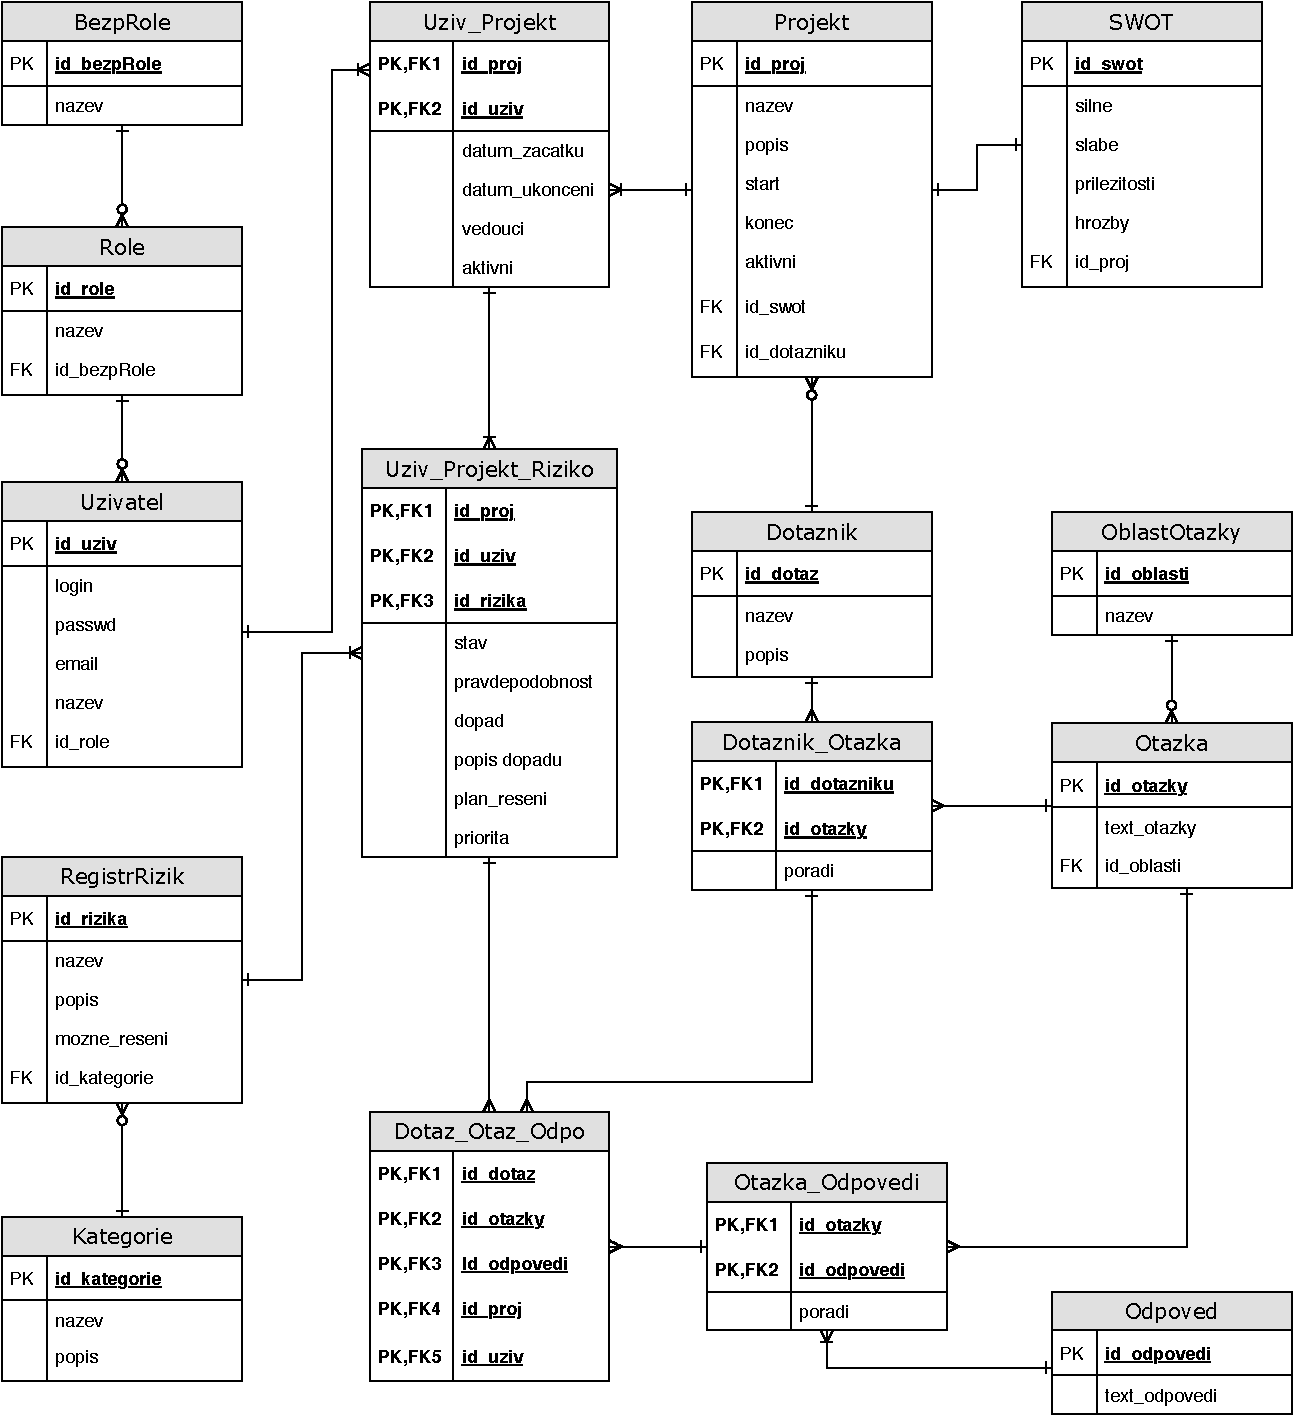
\includegraphics{obrazky-figures/database3.pdf}}
    \caption{Schéma struktury databáze [zdroj vlastní]}
    \label{schemaDB}
    \end{center}
    \end{figure}


\textbf{Uzivatel} je tabulka, která reprezentuje uživatele nástroje, půjde tedy buď o~člena týmu, projektového manažera nebo projektového administrátora. To, jakou roli uživatel bude mít určuje cizí klíč z~tabulky \textbf{Role}. Tabulka dále obsahuje přihlašovací informace daného uživatele včetně i hesla v~zašifrované podobě. Dále také i jeho pracovní email a jméno. Role umožňuje přidávat do systému další druhy rolí, jejím základem je ovšem \textbf{BezpRole}, která určuje tří základní bezpečnostní role - USER, MANGER a ADMIN, které se využívají pro určování přístupu ke zdrojům. Záznamy v~této tabulce nelze měnit.


\textbf{Projekt} určuje záznamy daného projektu. Ukládá se jeho název, základní popis, začátek prací a předpokládaný konec. Na daný projekt je pak navázaná tabulka \textbf{SWOT}, která obsahuje informace ze stejnojmenné analýzy. Tabulka projektu také obsahuje odkaz na dotazník, který je k~němu přiřazen. 

Aby bylo možné sledovat, kdo všechno je k~danému projektu přiřazen, tak mezi tabulkami Uživatel a Projekt je vazební tabulka \textbf{Uziv\_Projekt}, která dále umožňuje určit, kdy daný uživatel začal na projektu pracovat a kdy byl z~projektu odhlášen a také zda byl jeho manažerem či zůstal na projektu přihlášen až do jeho dokončení.

Tabulka \textbf{RegistrRizik} představuje centrální registr zjištěných rizik. V~tomto registru se uchovávají všechna unikátní rizika, která se kdy v~dané organizaci zjistila. Pomocí něho se může urychlit identifikace rizik na aktuálním projektu. Obsahuje název  rizika, jeho popis, možné obecné řešení a cizí klíč do tabulky \textbf{Kategorie}, která reprezentuje oblast, do které riziko spadá.

Vazební tabulka \textbf{Uziv\_Projekt\_Riziko} pak spojuje tabulky Uzivatel, Projekt a RegistrRizika. Umožňuje určit k~jakému projektu dané riziko patří a také kdo je jeho vlastníkem (neboli osobou odpovědnou za plnou identifikaci a analýzu rizika). Mezi další atributy patří pravděpodobnost jeho výskytu, míru a popis jeho dopadů, plán řešení, pokud se riziko vyskytne, jeho prioritu (může také označovat závažnost) a stav jeho identifikace a analýzy.

Pro lepší identifikaci rizik a jejich pozdější analýzu lze použít dotazníky. Tabulka \textbf{Dotaznik} je pak jejich reprezentací. Jaho atributy jsou název a krátký popis. Dotazník se může vyskytovat samostatně, případně může být přiřazen k~více projektům.

\textbf{Otazka} je tabulka, která obsahuje text potřebné otázky včetně i odkazu na oblast, které se otázka týká (tabulka \textbf{OblastOtazky}). Oblastí v~tomto případě již lze rozumět jako skutečné oblasti např. procesní, obchodní, technologická, rizika spojena ze zainteresovanými stranami atd.

Vytvořené otázky budou vždy uzavřené, při její tvorbě lze tedy využít již předem vytvořené možné odpovědi z~tabulky \textbf{Odpoved}. To, jaké bude mít otázka možné odpovědi se uchovává ve vazební tabulce \textbf{Otazka\_Odpovedi}, která zároveň obsahuje i atribut, který určuje pořadí dané odpovědi v~otázce.

Vazební tabulka \textbf{Dotaznik\_Otazka}, pak uchovává informace o~tom, jaké otázky se v~dotazníku vyskytují, přičemž atribut poradi určuje podobně jako v~tabulce Otazka\_Odpoved, pořadí dané otázky v~dotazníku. 

Celkové spojení uživatelů, projektů, dotazníků, otázek a odpovědí, pak symbolizuje vazební tabulka \textbf{Dotaz\_Otaz\_Odpo}. V~této tabulce se uchovávají informace o~tom, jak daný uživatel v~daném dotazníku na otázku odpovídal (jakou odpověď z~nabízených možných odpovědí vybral).

\section{Návrh uživatelského rozhraní}


Jak již bylo zmíněno dříve, výsledný nástroj má mít moderní vzhled s~responzivním designem. Při studium konceptů návrhů moderních webových stránek jsem nalezla informace o~Material Design od společnosti Google. Jedná se o~systém pravidel, návodů, nástrojů a~grafických komponent, které podporují návrh a vytváření moderních grafických uživatelských rozhraní. Hlavní stránka Material Design se pak dále zmiňuje, že se jedná o~vizuální jazyk spojující návrh s~inovativními myšlenkami z~oblastí technologie a vědy, jehož hlavní inspirace se nachází v~objektech reálného světa a jak tyto objekty reagují na přítomnost světla a stínu \cite{MaterialDesign}.

    \begin{figure}[!htbp]
    \begin{center}
    \scalebox{0.5}{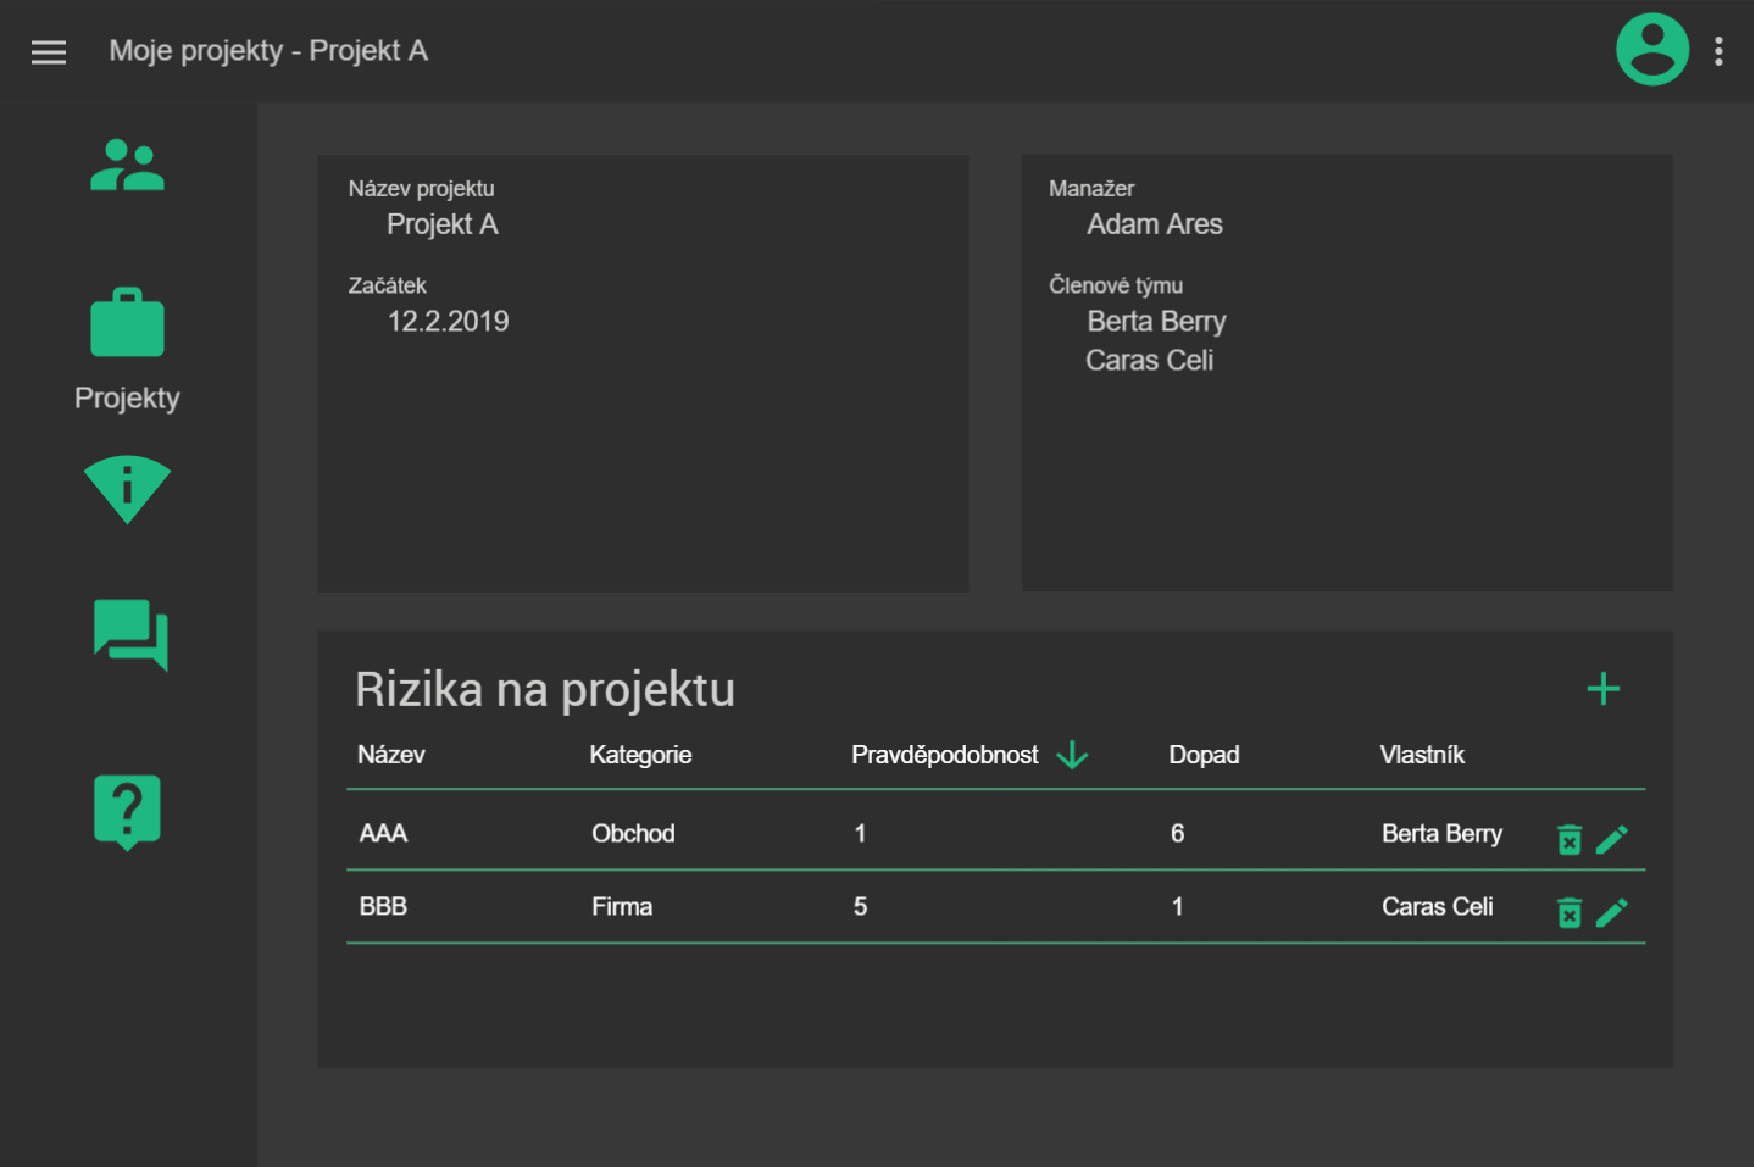
\includegraphics{obrazky-figures/Projekt.pdf}}
    \caption{Návrh karty projektu se zjištěnými riziky [zdroj vlastní]}
    \label{guiProjekt}
    \end{center}
    \end{figure}

Material Design dále nabízí i několik studií, jejichž cílem je prezentovat možnosti a~flexibilitu dostupných nástrojů a komponent. Návrh grafického uživatelského rozhraní této diplomové práce byl z~velké částí inspirován studiemi Rally \cite{Rally} a Reply \cite{Reply}.

Ke tvorbě zjednodušeného možného návrhu uživatelského rozhraní několika obrazovek byl použit online nástroj Fluid UI \cite{FluidUI}, který při tvoření návrhu umožňuje použití prvků ve stylu Material Design. Výsledný návrh obrazovky správy projektu lze vidět na obrázku \ref{guiProjekt}.

Dále byly vytvořené i zjednodušené návrhy obrazovek přihlášení do systému a správy dotazníků, které lze nalézt v~přílohách.
    
\chapter{Realizace a implementace}
\label{implementace}

V~této kapitole se popisuje implementace požadovaného nástroje a představuje se výsledná realizace. Ještě před začátkem implementace bylo nutné zvolit framework, v~českém překladu známý také jako aplikační rámec, který by odpovídal požadavkům návrhu, a to možnosti použití programovacího jazyku Java a umožnění odděleného vývoje klientské i~serverové části. Dále by měl být jednoduchý na konfiguraci, používání a ideálně také by měl poskytovat určitý stupeň zabezpečení přístupu. 

První část této kapitoly se zaměřuje na porovnání několika frameworků a knihoven pro naprogramování serverové i klientské části. Dále se pak blíže popisují zvolené programovací nástroje, a to je pak následováno popisem implementace a představení důležitých částí vytvořeného nástroje. 

\section{Vybrané aplikační rámce serverové části}

Jak se již dříve zmínilo, při výběru aplikačního rámce se zaměřilo na ty z~programovacího jazyka Java. Dle článků \cite{FBackend2} a \cite{FBackend1} se vybraly čtyři nejpoužívanější frameworky, které umožňují vytvářet serverovou část aplikace.

\subsection{Spring}

Spring framework (nebo některé z~jeho zjednodušených součástí) patří již po mnoho let na vrchol nejpoužívanějších aplikačních rozhraní jazyka Java. Lze ho použít ke full-stack řešení projektů, to znamená, že v~něm lze naprogramovat celou aplikaci od databáze až po grafické prvky klienta. Součástí frameworku je i Spring Security, který umožňuje snadnou implementaci autentizace i autorizace pomocí již existujících knihovních funkcí. Nevýhodou Spring frameworku může být jeho pomalejší učící křivka, případně zmatenost, kdy nějakou funkcionalitu lze naprogramovat více způsoby.

\subsection{Struts}

Struts framework je velice podobný Spring aplikačnímu rámci. Také využívá konceptu Model-View-Controller a taktéž se více hodí pro rozsáhlejší projekty. Struts se vyskytuje ve vice verzích – Struts 1 a Struts 2, přičemž více se využívá verze 2, která je rozšířená o~framework OpenSymphony. Hlavní výhodou může být aktivní dokumentace či centralizovaný systém konfigurace.

\subsection{Play}

Play je jednoduchý framework, který umožňuje vytvářet nástroje, které celkově mají malou velikost a ke funkčnosti potřebují pouze minimum zdrojů, čímž se hodí i pro vývoj mobilních aplikací. Jádro aplikačního rámce je naspáno v~jazyce Scala, ale umožňuje i podporu jazyka Java. Mezi výhody Play lze počítat plnou podporu NoSQL či neblokující vstup/výstupní operace. Tento framework používají společnosti EA, Walmart, Samsung a Linkedin.

\subsection{DropWizard}

Cílem DropWizard frameworku je umožnit vývojářům rychlou implementaci a nasazení výsledné aplikace. Velice se hodí k~implementaci REST aplikací či k~tvorbě mikroslužeb. Má také vestavěnou podporu validace dat a zabezpečení zdrojů pomocí autentizace a autorizace.

\section{Vybrané aplikační rámce klientské části}

Při vyhledávání možných frameworků, pomocí kterých bych mohla vytvořit klientskou část aplikace, jsem rychle objevila, že téměř všechny články řadí následující aplikační rámce na nejvyšší místa v~oblíbenosti.

\subsection{Angular}

Angular je framework založený na TypeScriptu, který je nadstavbou jazyka JavaScript a~přidává do něho statickou typovou kontrolu. Vychází z~aplikačního rámce Angular.js, ale není s~ním zpětně kompatibilní a je vyvíjen společností Google. Jednou z~výhod tohoto frameworku je, že má mnoho funkčnosti již vestavěných v~sobě. Nevýhodou pak může být jeho strmější učící křivka nebo složitější na porozumění dokumentace.

\subsection{React}
\label{reactFirst}

React je v~současnosti nejoblíbenější \uv{framework} pro tvorbu webových stránek. Je vyvíjen týmem ve společnosti Facebook. Často se mylně označuje jako framework, ale ve skutečnosti se jedná o~rozsáhlejší JavaScript knihovnu a z~tohoto důvodu musí vývojáři častěji doinstalovat dodatečné podpůrné knihovny. Výhodou Reactu je, že změna stavu jedné komponenty neovlivňuje jiné komponenty, nevýhodou pak může být, že z~důvodu vysoké oblíbenosti se knihovna velmi rychle rozvijí a vývojář tak může ztratit přehled o~všech změnách či vylepšeních.

\subsection{Vue.js}

Vue framework vyniká svojí jednoduchostí a malou velikostí výsledných souborů. Lze využít i ke tvorbě mobilních aplikací. Vue se v~některý případech používá i jako knihovna. Další výhoda je i v~jeho rozsáhlé dokumentaci. Nevýhodou může být, že komunita okolo tohoto aplikačního rámce není tak rozsáhla, jak v~předcházejících dvou.


\section{Zvolené programovací nástroje}

Na základě doporučení, jejich popularitě, počtu návodů a chuti se naučit novým technologiím, které bych mohla využit v~zaměstnání, jsem zvolila kombinaci \textbf{Spring Boot} \cite{Spring}, který je rozšířením Spring frameworku, pro serverovou část a \textbf{React} \cite{React} pro klientskou část.

\subsection{Spring a Spring Boot}

Jedním z~hlavních cílů Spring frameworku bylo poskytnout vývojářům nástroj pro zjednodušení a urychlení vývoje, jak jsem ale již výše zmínila, tento aplikační rámec získal postupem let mnoho funkčnosti rozložených do mnoha modulů, to ale způsobilo, že už i~založení projektů bylo zdlouhavé a muselo se speciálně dbát na správnou konfiguraci jednotlivých částí.

A~právě to byl jeden z~důvodů proč se vytvořilo rozšíření pro Spring framework\,--\,Spring Boot. Tento samostatný modul, který ale umožňuje využívat funkčnosti Spring aplikačního rámce, má za cíl ještě více urychlit vývoj aplikací a to tím, že většinu konfigurace provede automaticky nebo pomocí anotací. Také zjednodušuje přidávání nových modulů a závislostí, kdy stačí do konfiguračního souboru vložit pouze tzn. \texttt{starter} dané závislosti a Spring Boot se o~další nastavení postará sám. Názvy starterů některý modulů jsou: \texttt{spring-boot-starter-web}, \texttt{spring-boot-starter-security}, \texttt{spring-boot-starter-da\-ta-jpa}, atd. V~základu se také nachází již vestavěný server pro rychle testování či nasazení.


\subsubsection* {ORM, JPA a Hibernate}

\textbf{ORM} neboli \textit{Object-relational mapping}, v~překladu \textbf{Objektově relační mapování}, je programovací technika, která umožňuje pracovat s~databázi jako s~klasickými třídami a~objekty v~Javě (nebo jejich ekvivalenty v~ostatních objektově orientovaných jazycích). Dále také ORM poskytuje jistou úroveň odstínění druhu databáze od samotného programu, díky čemuž vývojář nemusí plně znát jazyk jakým se s~danou databázi komunikuje a v~případě potřeby také ulehčuje přechod z~jednoho typu databáze na druhý. Nevýhodou této techniky pak může být skutečnost, že vývojář plně \uv{nevidí} do procesů, které se na pozadí provádějí a také, že komunikace např. přímo v~SQL může být rychlejší a efektivnější než pomocí knihovny, která ORM implementuje.

\textbf{JPA} je součástí standartu Java a byla známá pod názvem \textit{Java Persistence API}. Když ale Java Enterprise Edition (Java EE) změnila název na Jakarta EE, tak bylo JPA přejmenováno na \textit{Jakarta Persistence}. Jedná se o~specifikaci ORM pro Javu, ve kterém se specifikují rozhraní a anotace používané pro mapování objektů a vztahů mezi objekty do databáze. Mezi nejznámější anotace JPA patří: \texttt{@Entity} a \texttt{@Table} pro definici tabulek, \texttt{@Id} pro identifikaci primárního klíče \texttt{@OneToOne}, \texttt{@OneToMany}, \texttt{@ManyToOne}, \texttt{@ManyToMany} pro provázání tabulek pomocí cizích klíčů.

\textbf{Hibernate}, známý také jako \textbf{Hibernate ORM}, je framework, který implementuje ORM pro jazyk Java, zároveň také implementuje specifikaci JPA. Mapování objektů, lze provést pomocí XML souborů nebo pomocí anotací. Hibernate také poskytuje modul pro validaci dat, podporu pro persistenci dat v~datových skladištích NoSQL a mnohem více  \cite{Hibernate}.

Spring Boot používá Hibernate jako výchozí implementaci JPA. Výchozí data se do tabulek načtou ze SQL skriptu import.sql, který Spring Boot automaticky spustí po vytvoření databáze. Algoritmus \ref{anotace} zobrazuje příklad třídy s~JPA anotacemi, ze kterých Hibernate vytvoří odpovídající tabulku (algoritmus \ref{hibernateSQL} představuje kód, který vytvoří Hibernate). Starter pro všechny závislosti potřebné k~používaní Hibernate se jmenuje \texttt{spring-boot-starter-\\data-jpa}.



\begin{lstlisting}[caption={Třída s~anotacemi},captionpos=b,frame=single, ,label=anotace]
@Entity(name = "user")
@Table(name = "User")
public class User {

    @Id
    @GeneratedValue(strategy = IDENTITY)
    @Column(name = "id", unique = true, nullable = false)
    private long id;

    @Column(name = "login")
    private String login;

    @Column(name = "passwd")
    private String passwd;

    @Column(name = "email")
    private String email;

    @ManyToOne
    @JoinColumn(name = "fk_role", nullable = false)
    private Role role;

}
\end{lstlisting}

\begin{lstlisting}[caption={SQL kód vygenerovaný Hibernate},captionpos=b,frame=single, ,label=hibernateSQL]
 create table user (
    id bigint generated by default as identity,
    email varchar(255),
    login varchar(255),
    passwd varchar(255),
    fk_role bigint not null,
    primary key (id)
)
    
alter table user 
    add constraint FKp61v76usu5tblw5in3jlpe8rc 
    foreign key (fk_role) 
    references role
\end{lstlisting}

\subsubsection* {MVC a REST}

\textbf{MVC} je zkratka pro spojení slov \textit{Model-Viev-Controller} a jedná se o~softwarovou architekturu, která doporučuje rozdělení aplikace do tří modulů, které jsou na sobě navzájem nezávislé.  Model, lze chápat jako datový model či datová vrstva, jejím úkolem je uchovávat data aplikace. View neboli prezenční vrstva zobrazuje uživateli data, které ji dle potřeby zpřístupní datová vrstva. Controller lze přeložit jako řídící vrstva, je to vrstva nacházející se mezi datovou a prezenční vrstvou, jejím úkolem je řídit aplikaci, reagovat na požadavky pocházející z~prezenční vrstvy a o~případných změnách v~datech informovat datovou vrstvu. 

\textbf{REST}, neboli \textit{Representational State Transfer}, popisuje principy pro jednoduchý přenos dat (zdrojů aplikace) mezi klientem a severem. V~REST specifikaci každý zdroj uložený na serveru má své jedinečné URI (Uniform Resource Identifier, jednotný identifikátor zdroje) pomoci kterého lze k~němu přistupovat. S~každým zdrojem pak lze provádět čtyři následující operace – vytvoření, čtení, editace a smazání, což jsou přesně CRUD operace. Ke komunikaci s~REST aplikací lze použít internetový protokol HTTP, kde se využijí jeho metody GET, POST, PUT, DELETE, atd. Data mezi klientem a serverem se pak mohou posílat ve formátu XML, XHTML či JSON.

K~aktivaci MVC ve Spring Boot aplikaci se používá starter \texttt{spring-boot-starter-web}, který ze Spring frameworku naimportuje modul Spring MVC, pomoci kterého lze vytvářet tzv. RESTful aplikace (neboli aplikace implementující REST přístup ke zdrojům. Díky web starteru se také zpřístupní další požadované technologie pro vývoj webové aplikace:  vestavěný Tomcat server, knihovnu Jackson pro práci s~daty ve formátu JSON,  validátor dat a další.

\subsubsection* {Spring Security}

Pro zabezpečení přístupu k~datům aplikace používá Spring Boot modul \textbf{Spring Security}, který se importuje starterem \texttt{}{spring-boot-starter-security}. Spring Security poskytuje jak autentizaci, tak i autorizaci (ověření identity uživatele a ověření, zda daný uživatel má povolení danou akci provádět). Jednotlivé požadavky přicházející na server musí ještě před tím, než dojdou ke Controlleru, projít řadou filtrů nastavených pomocí Spring Security. Pokud požadavek některým z~filtrů neprojde, tak je odmítnut, typicky se pak klientské straně přepošle negativní odpověď se stavovým kódem 401, který se v~HTTP protokolu používá ke naznačení, že uživatel není autentizován. 

Spring Security poskytuje i další funkčnost jako zapamatování přihlášení či zašifrování hesla v~databázi a při přenosu. Řeší také známé slabiny, které se při komunikaci mezi klientem a serverem mohou vyskytnou. Příkladem může být \textbf{CRSF} neboli \textit{cross-site request forgery}, kdy útočník zneužije spojení mezi aktuálně přihlášeným uživatelem a serverem. Pomocí tohoto spojení pak může odeslat požadavky, o~kterých si server myslí, že se jednají o~legitimní požadavky uživatele. Problém je možné řešit tak, že po autentizaci klienta si obě strany synchronizují tzn. CRSF token, který klientská strana přidává ke požadavkům a zabezpečení serveru tento token ověřuje. Díky tomuto zabezpečení pak server přesně zná původ požadavku.  

\subsection{React}

Jak jsem již zmínila, React je JavaScript knihovna pro tvorbu interaktivních uživatelských rozhraní. React umožňuje vytvářet samostatné znovupoužitelné komponenty (prvky uživatelského rozhraní), které jsou schopné spravovat svůj vnitřní stav. Jednoduché komponenty pak lze skládat do složitějších. React využívá konceptu \textbf{virtuálního DOM} a \textbf{JSX}. 

\textbf{Virtuální DOM} (\textit{Document Object Model}, \textbf{objektový model dokumentu}) staví na konceptu uložení virtuální reprezentaci v~paměti a jeho následné synchronizace se skutečným DOM. React ho využívá k~tomu, aby DOM vždy odpovídal stavu jednotlivých komponent \cite{VDOM}.

\textbf{JSX} je syntaktické rozšíření JavaSriptu a slouží k~definování vzhledu komponent v~Reactu. Díky JSX může být definice vzhledu a funkce zodpovědné za logiku komponenty pohromadě v~jednom souboru. Použitím JSX se také zabraňuje útokům typu \textbf{XSS} (\textit{Cross-site scripting}), kdy se útočník snaží přes nějaký neošetřený vstup nahrát na stránku nežádoucí skript. Algoritmus \ref{jsxAlg} ukazuje použití JSX, právě prvek \texttt{React DOM} zajišťuje, že útok XSS nelze provést \cite{JSX}.

\begin{lstlisting}[caption={Příklad JSX, vykreslení prvku H1 do HTML komponenty s~id root},captionpos=b,frame=single, ,label=jsxAlg]
const name = 'Josh Perez';
const element = <h1>Hello, {name}</h1>;

ReactDOM.render(
  element,
  document.getElementById('root')
);
\end{lstlisting}

\subsection{Další důležité knihovny}

V~sekci \ref{reactFirst} jsem se zmiňovala, že k~Reactu se často musí doinstalovat další knihovny. V~této sekci popisuji další nejdůležitější knihovny používané v~této diplomové práci. Celý soupis použitých knihoven pro tvorbu uživatelského rozhraní lze nalézt v~příloze TODO.

\subsubsection *{Material-UI}

Material-UI je nejpopulárnější knihovnou pro tvorbu uživatelského rozhraní vytvořenou pro React. Obsahuje mnoho již předem vytvořených prvků, které splňují požadavky kladené specifikací Material Design. Jedná se o~alternativu ke knihovně Bootstrap. Prakticky celý nástroj využívá komponenty z~této knihovny. Taktéž všechny použité ikony jsou převzaty z~Material-UI icons.

\subsubsection *{Material-table}

Knihovna materiál-table rozšiřuje komponentu tabulky z~Material-UI a přidává do ní dodatečnou funkčnost. Poskytuje jednodušší přidávání, editaci a mazání záznamů. Dále také umožňuje vyhledávání v~záznamech, filtraci a třídění dat, zobrazování panelu s~detaily, export do požadovaných záznamů a mnohem více. Výchozí chování jednotlivých funkčností lze předefinovat dle potřeb uživatele.

\subsubsection *{Nivo}

Nivo je knihovna grafových komponent pro React. Obsahuje značné množství nejpoužívanějších druhů grafů, které lze v~případě potřeby upravovat. Všechny grafy jsou interaktivní, obsahují i legendy a každý z~nich má i verzi, která je responzivní ke změně velikosti okna. Nivo má na svých stránkách i velice zajímavou interaktivní dokumentaci, ve které lze měnit parametry atributů daného grafu, které se okamžitě promítají do vykreslené komponenty. 

\subsubsection *{Redux a React-Redux}

V~Reactu funguje předávání informace z~rodičovské komponenty na dceřinou. Problém se může vyskytnou, pokud stejnou informaci potřebují dvě odlišné komponenty, které nejsou ve stejné větvi, případně ty, co jsou ve stejné větvi, ale jedná je od druhé až příliš moc vzdálená a pro ostatní komponenty je daná informace nepotřebná. 

Redux je nástroj pro správu stavu aplikaci, který daný stav ukládá do speciálního objektu \texttt{store}, ze kterého mohou všichni číst. V~rámci Reduxu se pak hovoří ještě o~\texttt{actions} a \texttt{reducers}. Actions lze uvažovat za událostí, které říkají, že se má provést nějaká akce. Každá akce je definovaná svým typem a obsahem (payload) přenášeným z~aplikace do store. Reducers jsou pak funkce, které dle dané action provedou nějakou modifikaci s~daty, co se nacházejí ve store a vrátí nový stav.

React-Redux byl vytvořen pro spojení Reactu a Reduxu. Přidává do aplikace komponenty a funkce díky kterým mohou všechny komponenty aplikace přistupovat ke stavům ve store a také vyvolávat akce, které store modifikují.

\subsubsection *{Formik a Yup}

Formik je pomocná knihovna pro správu formulářů. Jejím hlavním úkolem je získávání dat z/do stavů formuláře, validace zadaných hodnot, zobrazování chybových zpráv a zpracování potvrzení formuláře. 

Yup je knihovna pro validaci zadaných hodnot. Umožňuje vytvořit validační schéma pro různé typy objektů a hodnoty. Formik používá knihovnu Yup jako výchozí validátor. 

\subsubsection *{Axios}

Axios je jednoduchý HTTP klient pro komunikaci s~REST API. Lze ho používat s~Reactem nebo s~libovolně jiným frameworkem. Axios je velice podobné fetch API z~JavaScriptu, které umožňuje pohodlnější práci s~AJAX (\textit{Asynchronous JavaScript and XML}) dotazy a také vrací tzn. \texttt{Promise} objekt, který slouží jako příslib, že jednou v~něm budou vrácená přijatá data.

\subsubsection *{React Router}

React Router je jednoduchá knihovna, pomocí které lze řešit směrování na různá URL aplikace.

\subsection{Podpůrné programovací nástroje}

Při tvorbě implementace klientské i serverové částí se použilo IDE IntelliJ IDEA od společnosti JetBrains.
Při dolaďování vstupů a výstupu API se pak použil program Postman, který umožňuje tvořit HTTP dotazy, poslat je na server a následně zobrazí odpověď, kterou vyslal server.


\section{Implementace nástroje}

Aplikace je rozdělen na dvě částí, klientskou a serverovou. Klientská část je naprogramovaná pomocí JavaScript knihovny React, serverová pak využívá Java aplikační rámec Spring Boot, kde nejdůležitějšími moduly jsou Spring Data JPA, Spring MVC a Spring Security.

\subsection{Server}

Server se využívá jako RESTful API (\textit{Application Programming Interface}), neboli se využívá jako webová služba, která reaguje na HTTP požadavky GET, POST, DELETE.

Metoda GET se používá pro získávání zdrojů ať už se jedná o~jedinou položku nebo seznam několika z~nich. POST se využívá ve dvou případech, a to, pokud se nahrávají nová data anebo se data modifikují. DELETE slouží pro smazání požadované položky.

Server je rozdělený do pěti částí\,--\,\texttt{security}, \texttt{web}, \texttt{service}, \texttt{repository} a \texttt{domain}. Každý validní požadavek, který na server přijde, je svázán nebe musí postupně projít každou z~částí.

\subsubsection *{Domain}

V~adresáři domain se nacházejí soubory s~definicemi tříd, které byly vytvořený dle návrhu databáze, který byl popsán v~části \ref{databaze}. Ke třidám jsou pak přidány potřebné anotace, podle kterých Hibernate vytvoří odpovídající tabulky v~databázi. Nejpoužívanější anotace pro definici tabulek jsou: 

\begin{itemize}
    \item \texttt{@Entity} a \texttt{@Table} specifikují, že daná třída je entita, kterou lze namapovat na tabulku, s~\texttt{@Table(name = "Jmeno")} se také udává název tabulky.
    \item \texttt{@Id} a \texttt{@GeneratedValue(strategy = IDENTITY)} se používají pro naznačení který atribut třídy má být primárním klíčem entity a také definují strategii pro automatické generování hodnoty klíče.
    \item\texttt{@Column(name = "jmeno", nullable = false, columnDefinition="text")} definuje atribut třídy, který se má ukládat do databáze, vlastnost name udává název pod jakým se má vytvořit, nullable označuje zda hodnota může nabývat null hodnot a~columnDefinition pak určuje typ.
\end{itemize}

Každý vztah mezi tabulkami je dvousměrný, tzn. že spojené třídy mají na sebe navzájem odkazy. V~databázi ovšem bude mít jenom jedna z~nich cizí klíč druhé tabulky. Toto spojení zajišťují anotace \texttt{@OneToMany} a \texttt{@ManyToOne} s~\texttt{@JoinColumn}. Příklad \ref{roleOneToMany} zobrazuje použití \texttt{@OneToMany} ve třídě \texttt{Role} nad atributem, který uchovává uživatele s~danou rolí, \texttt{mappedBy} pak říká, že vlastníkem daného sloupce je jiná entita – tabulka nebude obsahovat cizí klíč.
Použití inverzní anotace \texttt{@ManyToOne} s~\texttt{@JoinColumn} ukazuje příklad \ref{uzivatelManyToOne}, kde jsou použity nad atributem uchovávajícím odkaz na roli uživatele. Vlastnost \texttt{name} udává název sloupce s~cizím klíčem.

\begin{lstlisting}[caption={Použití anotace pro vytvoření vztahu na straně tabulky Role},captionpos=b,frame=single, ,label=roleOneToMany]
@OneToMany(mappedBy = "role", cascade = CascadeType.ALL, 
orphanRemoval = true)
private List<Uzivatel> uzivatele = new ArrayList<Uzivatel>();
\end{lstlisting}

\begin{lstlisting}[caption={Použití anotace pro vytvoření vztahu na straně tabulky Uživatel},captionpos=b,frame=single, ,label=uzivatelManyToOne]
@ManyToOne
@JoinColumn(name = "fk_role", nullable = false)
private Role role;
\end{lstlisting}

V~domain se také nacházejí další dva adresáře. Adresář id obsahuje definice složených primárních klíčů, které využívají některé spojené tabulky. Složený klíč tvoří třída, která je anotovaná \texttt{@Embeddable}, pomocí \texttt{@EmbeddedId} se pak objekt dané třídy označí jako klíč.

Druhým adresářem je serializer, který obsahuje definice pro transformování dat na JSON formát. Spring Boot má svůj vlastní výchozí serializér, který ale z~důvodů dvousměrného odkazu může vytvořit nekonečnou smyčku dat. To, zda se má při serializaci použít vlastní serializér, se značí anotací \texttt{@JsonSerialize(using = RoleSerializer.class)}.

\subsubsection *{Repository}

Adresář repository obsahuje soubory s~rozhraním (interface), které rozšiřuje \texttt{JPARepository} z~modulu Spring Data JPA. Rozhraní jsou vytvořená pro každou třídu z~domain a jsou označená anotací \texttt{@Repository}. JPARepository zpřístupňuje základní metody pro komunikaci s~databázi neboli uložení jednoho či více záznamů, podobně pak vyhledávání a mazání dle id a mnohem více. Co se týče ukládání, tak JPARepository rozeznává ukládání nového objektu od editace existujícího pomocí toho, zda atribut, který je označen jako primární klíč, má hodnotu \texttt{null} či jinou.

Spring Data JPA umožnuje také vytvářet vlastní metody pro přístup např.: \texttt{findByIdId\-ProjektuAndIdIdRizika(long idProjektu, long idRizika)} pro nalezení záznamu, jehož id je rovné idProjektu a idRizika. Takto vytvořené metody se ve Spring Data JPA dokumentaci nazývají \textit{Query metody}.

\subsubsection *{Service}

V~adresáři service se nacházejí soubory se třídami, které mají anotaci \texttt{@Service}. V~těchto souborech lze najít funkce, které mají na starosti úpravu dat před tím, než se zavolá odpovídající repository objekt, který dané úpravy promítne do databáze.  Jedná se tedy o~tzn. bussiness vrstvu, která obsahuje logiku celé aplikace. Tato funkčnost je velmi často spojována s~funkčností řadiče (\textit{controller}), je ovšem doporučeno jejich oddělení, díky čemuž, pokud se změní druh databáze, tak se budou muset změnit pouze funkce ve \texttt{@Service}. Dále to také umožňuje oddělení logiky od zpracování příchozího požadavku, díky čemuž bude mít řadič na starosti pouze příjem dat a vracení výsledku dotazu.

Všechny třídy využívají mechanismu automatického vkládání závislého repository objektu (\textit{dependency injection}), pomocí kterého se přikazují změny v~databázi. Toto vkládání umožňuje anotace \texttt{@Autowired}. 
V~každé \texttt{@Service} třídě se vyskytují minimálně tyto čtyři metody:
\begin{itemize}
    \item \textbf{saveOrUpdate} pro ukládání nového či pozměněného objektu
    \item \textbf{findAll} pro vyhledání všech objektů
    \item \textbf{findById} pro vyhledání jednoho objektu podle jeho id
    \item \textbf{delete} pro smazání požadovaného objektu
\end{itemize}

FindAll, findById a delete jsou ve většině případů pouze jednoduché funkce, které předávají příkaz z~řadiče do repository objektu. SaveOrUpdate metody provádějí ještě dodatečné úpravy dat před jejich uložením.

Dodatečnými úpravami se zde myslí, že pokud např. objekt má v~jednom z~atributů odkaz na jinou instanci (neboli záznam v~tabulce obsahuje cizí klíč jiné tabulky), tak při tvorbě tohoto objektu z~dat ve formátu JSON (provádí se v~řadiči k~adresáři web) bude u~odkazované instance inicializovaná pouze jeho hodnota id. Z~toho důvodu se musí dodatečně z~databáze získat objekt s~daným id a přiřadit se k~právě tvořené instanci. 

Dalším případem je, pokud se ukládá pouze modifikace již existujícího objektu. Přijatá instance neobsahuje seznamy všech objektů, se kterými je ve vztahu. Pokud by ale daný objekt v~databázi, který chceme modifikovat, nějaké vztahy měl, ale při ukládání jeho novější verzi je neměl nastavené, tak by systém uvažoval, že je má ze společných tabulek smazat. Z~toho důvodu se musí, ještě před uložení objektu, vybrat z~databáze starou verzi, zkopírovat potřebné seznamy do nové verze.

Další úpravy při ukládání se provádí také pokud právě ukládaný objekt nějakým způsobem ovlivňuje záznamy, které se v~databázi již nacházejí. V~tomto případě, se nejdříve musí načíst ovlivněné objekty, pozměnit jejich atributy a uložit je. Až po této sekvenci kroků, se nový objekt uloží.


\subsubsection *{Web}

Adresář web obsahuje řadiče, které určují API serveru. Každá třída řadiče je anotována s~\texttt{@RestController} a \texttt{@RequestMapping}. \texttt{@RestController} určuje, že řadič přijímá REST požadavky. \texttt{@RequestMapping} pak nastavuje prefix API, kterým je \textbf{api/nprr}. Podobně jako třídy v~service i tady se v~na začátku každé třídy vkládá závislý objekt, tentokrát ale je jeho instance ze service. Každá metoda třídy řadiče obsluhuje jeden požadavek a anotace nad ní pak určuje, na jaký druh HTTP metody reaguje a také ji přiděluje suffix adresy pro získání zdroje. Používané anotace určující druh HTTP metody jsou následující:

\begin{itemize}
    \item \texttt{@PostMapping("/project")} pro POST požadavky, v~tomto případě se jedná o~uložení nového nebo editaci již existujícího projektu.
    \item \texttt{@GetMapping("/projects")} pro GET požadavky, zde jako získání všech projektů.
    \item \texttt{@DeleteMapping("/project/\{id\}")} pro DELETE požadavky, zde pro smazání projektu s~daným id.
\end{itemize}

 Metody řadiče pak na požadavky odpovídají seznamem \texttt{Iterable}, pokud se jedná o~GET požadavek na získání více záznamů, anebo pomocí objektu \texttt{ResponseEntity}, který reprezentuje celý objekt HTTP odpovědi a umožňuje nastavit jeho hlavičku, tělo a návratový kód. 
Při POST požadavcích (příklad \ref{roleController}) metody řadiče přijímají objekt, který se má uložit do databáze. Tento objekt je původně ve formátu JSON, ale pomocí anotace \texttt{@RequestBody} se provede automatická deserializace na požadovaný formát objektu. \texttt{@Valid} pak aktivuje validaci atributu u~kterého se nachází. To jaká pravidla musí atribut validovaného objektu splňovat určují anotace použité při definování třídy v~domain např. \texttt{@NotBlank(message = "Název role musí být zadán")}, který určuje, že daný String atribut nemůže být prázdný. V~případě, že validace skončí neúspěchem, tak se její výsledek společně s~chybovými zprávami nachází v~objektu \texttt{BindingResult}.

\begin{lstlisting}[caption={Metoda řadiče pro uložení nového či editovaného objektu Role},captionpos=b,frame=single, ,label=roleController]
@PostMapping("/role")
public ResponseEntity<?> addRole(@Valid @RequestBody Role role, 
    BindingResult result) {
    ResponseEntity<?> errors = SpolecneFunkce.errorCheck(result);
    if (errors != null)
        return errors;
    Role newRole = roleService.saveOrUpdate(role);
    return new ResponseEntity<Role>(newRole, HttpStatus.CREATED);
}
\end{lstlisting}

Pro naznačení, kterého objektu se dotaz týká, např. získání projektu jehož id je 1 se v~parametrech obsluhujících metod označuje anotací \texttt{@PathVariable}. Díky tomu lze pak mít nad metodou anotaci s~např. \texttt{@DeleteMapping("/project/{id}")}, která se při volání z~klienta použije jako \textbf{/project/1}. V~případě, že se objekt s~daným id v~databázi nenachází, tak se vrátí objekt \texttt{ResponseEntity} se stavovým kódem \textbf{404}, který se v~HTTP používá pro označení, že daný dokument není nalezen. 

Odpověď s~kódem 404 se také vrátí v~případě, že server přijme požadavek, pro který ale neexistuje obsluhující metoda.

Seznam všech dostupných API lze nalést v~příloze. TODO udělej přílohu

\subsubsection *{Security}

Jak se již dříve zmiňovalo, zabezpečení aplikace zajišťuje modul Spring Security. Soubory týkající se zabezpečení se nacházejí v~adresáři security. Konfigurace zabezpečení se provádí v~souboru \texttt{SecurityConfiguration.java}. Přihlašování probíhá pomocí přihlašovacího formuláře a server očekává, že obdrží tři parametry – \texttt{username}, \texttt{password} a \texttt{remember}, kde remember má serveru napovědět, zda si pamatovat přihlášení uživatele. Server má nastaveno (soubor \texttt{MyAuthSuccessHandler.java}) aby při neaktivitě delší než \textbf{60 vteřin} uživatele automaticky odhlásil. Neaktivitou se myslí, že klient neodešle po dobu 60-ti vteřin žádný požadavek. Při zapamatování, se ale po přihlášení uživateli odešle cookie soubor, klient pak toto cookie připojuje ke každému požadavku, takže i když server odhlásí uživatele z~důvodu neaktivity, tak po dobu platnosti tohoto cookie, server nebude znovu vyžadovat přihlášení. 

Pro CSRF ochranu se také využívá cookie soubor. Server daný ochranný token pošle ve formě cookie. Klient pak tento token odesílá ve hlavičce každého POST požadavku.



\subsection{Klient}

Při představování technologií jsem zmiňovala, že základem klientské částí je knihovna React. Aplikace se váže na HTML dokument pomocí \texttt{id} atributu \texttt{root} v~\texttt{index.html}, který se nachází v~adresáři public. Funkci navázání lze pak nalézt v~hlavní zdrojové složce klienta src v~souboru \texttt{index.js} pojmenovanou jako \texttt{ReactDOM.render()} (příklad této funkce již byl k~vidění dříve na příkladu \ref{jsxAlg}), která připojuje komponentu \texttt{App} obsahující celou aplikaci.

Na začátku je ještě vhodné zmínit co všechno se do systému Redux, který byl vysvětlen dříve v~této kapitole, ukládá a jak se používá. Objekt \textit{store} se vytváří ještě před tím, než se celá aplikace načte a při jeho tvorbě se používá kombinovaný objekt \textit{reducer}, který zpřístupňuje všechny funkce na změnu stavu. Store se pak zpřístupňuje komponentě App a~všem jejím potomkům, pomocí komponenty \texttt{Provider}, která ji obaluje. Používá se hlavně pro ukládání informací o~projektu, jehož informace se mají zobrazit – základní údaje, kdo je manažer projektu a kdo řešitel, celková velikost projektového týmu, počet dnů do dokončení, informace o~rizicích identifikovaných na projektu a také data dotazníku jež k~němu byl přiřazen. Dále se také ukládají informace samotné aplikace – jaký mód je aktivní (světlý nebo tmavý), titulek aktivního okna, zda je menu otevřené nebo zavřené nebo zda se na serveru vyskytla chyba a klient musí zobrazit chybovou stránku. Dodatečně se do store ukládají i informace o~aktivním uživateli jako je jeho id a role. Actions a reducers, které Redux používá se nacházejí ve svých odpovídajících adresářích actions a reducers. 

Komponenty se primárně nacházejí v~adresáři components, kde jsou rozdělené podle toho, jakou část aplikace tvoří. Nástroj lze rozdělit na sedm částí – \textbf{přihlašování}, \textbf{dashboard}, \textbf{správa uživatelů}, \textbf{projekty}, \textbf{centrální registr rizik}, \textbf{dotazníky}, \textbf{otázky} a~\textbf{odpovědi}. 

Většina koncových komponent je samostatných, což znamená, že si sami načítají případně odesílají nová nebo modifikovaná data pomocí knihovny axios.

V~aplikaci se často zobrazují data formou záznamů v~tabulkách. Každá tabulka umožňuje dynamické vyhledávaní v~načtených záznamech pomocí vyhledávacího pole. Taktéž lze v~každé provádět přidávání, mazání a editaci dat. Pro přidání a editaci záznamu se otevře dialog s~odpovídajícími políčky. Pokud všechny zadané hodnoty budou validní, tak se při uložení provedou provedou následující dvě akce – data se odešlou v~požadovaném formátu na server pomocí axios s~metodou POST a zadané hodnoty se vrátí to komponenty tabulky, kde se zobrazí nový nebo editovaný záznam. Sloupce v~tabulkách lze uchytit a přesunout na místo jiného sloupce, případně lze hodnoty v~každém z~nich seřazovat vzestupně nebo sestupně dle abecedy.

\subsubsection *{Přihlašování}

Při načtení se aplikace snaží ze serveru získat informace o~uživateli.  Pokud server vrátí kód 401 s~tím, že uživatel není přihlášen, tak se zobrazí stránka s~přihlašovacím formulářem, který tvoří komponenta \texttt{LoginForm}. V~opačném případě, bude uživatel automaticky přesměrován na svou uvítací stránku~\,--\,~dashboard. Pokud se z~autentizace na serveru opět vrátí 401 zobrazí se informace, že uživatel zadal špatné přihlašovací údaje. Při přihlašování lze vybrat možnost zapamatovat si aktuálně přihlášeného uživatele.

\subsubsection *{Boční menu a panel aplikace}

Hlavní panel aplikace obsahuje ikonová tlačítka pro otevření a zavření bočního menu, přepnutí na světlý a tmavý mód a také tlačítko na odhlášení uživatele. To, zda je menu zavřené nebo otevřené se ukládá do Redux store, odkud si to následně komponenta \texttt{MenuAppBar} stáhne. Panel aplikace také obsahuje název, který určuje aktuální polohu v~aplikaci, i tento název získává komponenta ze store.
Přístup k~jednotlivým částem nástroje je ovlivněn rolí, která byla uživateli přidělena. Uživatel s~bezpečnostní rolí ADMIN má přístup ke všem částem aplikace. MANAGER a USER pak mají, co se týče menu, omezený přístup pouze k~Dashboard, Projekty a Registr rizik. Rozdíl mezi otevřeným a uzavřeným menu lze vidět na obrázku \ref{menu}. Na stejném obrázku se také nachází rozdíl zobrazení menu pro uživatele ADMIN a pro všechny ostatní role. 

    
\begin{figure}[h]
    \begin{minipage}{.333\linewidth}
    \centering
    \subfloat[Uzavřené]{\label{main:a}
\includegraphics[scale=.99]{obrazky-figures/menuClose.png}}
    \end{minipage}%
    \begin{minipage}{.333\linewidth}
    \centering
    \subfloat[Otevřené]{\label{main:b}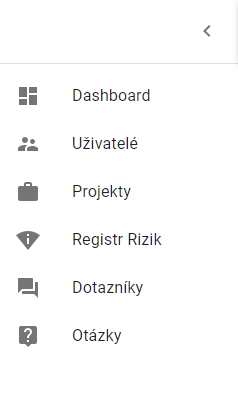
\includegraphics[scale=.75]{obrazky-figures/menuOpen.png}}
    \end{minipage}
    \begin{minipage}{.333\linewidth}
    \centering
    \subfloat[Jiná role]{\label{main:c}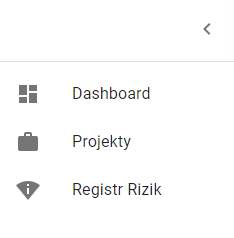
\includegraphics[scale=.75]{obrazky-figures/menuMana.png}}
    \end{minipage}
    \caption{Porovnání uzavřeného a otevřeného menu role ADMIN s~menu ostatních rolí [zdroj vlastní]}
    \label{menu}
\end{figure}
 


\subsubsection *{Dashboard}

Komponenty týkající se Dashboardu se nacházejí v~adresáři dashboard. Stránka se nachází na adrese \textbf{/app/dashboard}. Hlavní komponentou je \texttt{DashboardPage}, pomocí které se dashboard rozděluje na dvě částí – levou a pravou. 

Pravou část tvoří komponenta \texttt{Profile}, která zobrazuje profil aktuálně přihlášeného uživatele. Na kartě profilu se nacházejí základní informace uživatele – jeho jméno a příjemní, e-mail a aktuálně přiřazená role. 

Levá komponenta se pak liší dle přiřazené bezpečnostní role. Každá role má svou vlastní komponentu – \texttt{UserPart}, \texttt{ManagerPart}, \texttt{AdminPart}. V~kódu \texttt{DashboardPage.js} se ještě před tím, než se vloží do DashboardPage, tak se vytvoří pomocné objekty, které se inicializují funkcemi, které pomocí informací ve Redux store určí, zda komponentu vykreslit nebo místo ní vrátí hodnotu \texttt{null}, která nic nezobrazuje. Ačkoliv jsou všechny tři objekty vložené, tak se vykreslí pouze jeden z~nich. 

Uživateli s~rolí USER se zobrazují karty aktivních projektů, ke kterým je přiřazen. Karta obsahuje název projektu, datum, kdy k~němu byl uživatel přidělen a odkaz, který uživatele přenese na stránku s~informacemi o~daném projektu. MANAGER uživateli se zobrazují aktivní i neaktivní projekty, které řídil. V~jeho případě se na kartách aktivních projektů zobrazuje jeho počáteční datum. U~ukončených projektů pak jejich datum uzavření. U~role ADMIN se kromě aktivních a neaktivních projektů zobrazují i informace o~počtu uživatelů v~databázi a počtu rizik v~centrálním registru rizik. Obrazovku dashboardu administrátora lze vidět na obrázku \ref{dashboardObrazek}. Pokud v~databázi nebudou pro danou část data, tak se zobrazí odpovídající informace o~chybějících datech.

    \begin{figure}[ht]
    \begin{center}
    \scalebox{0.3}{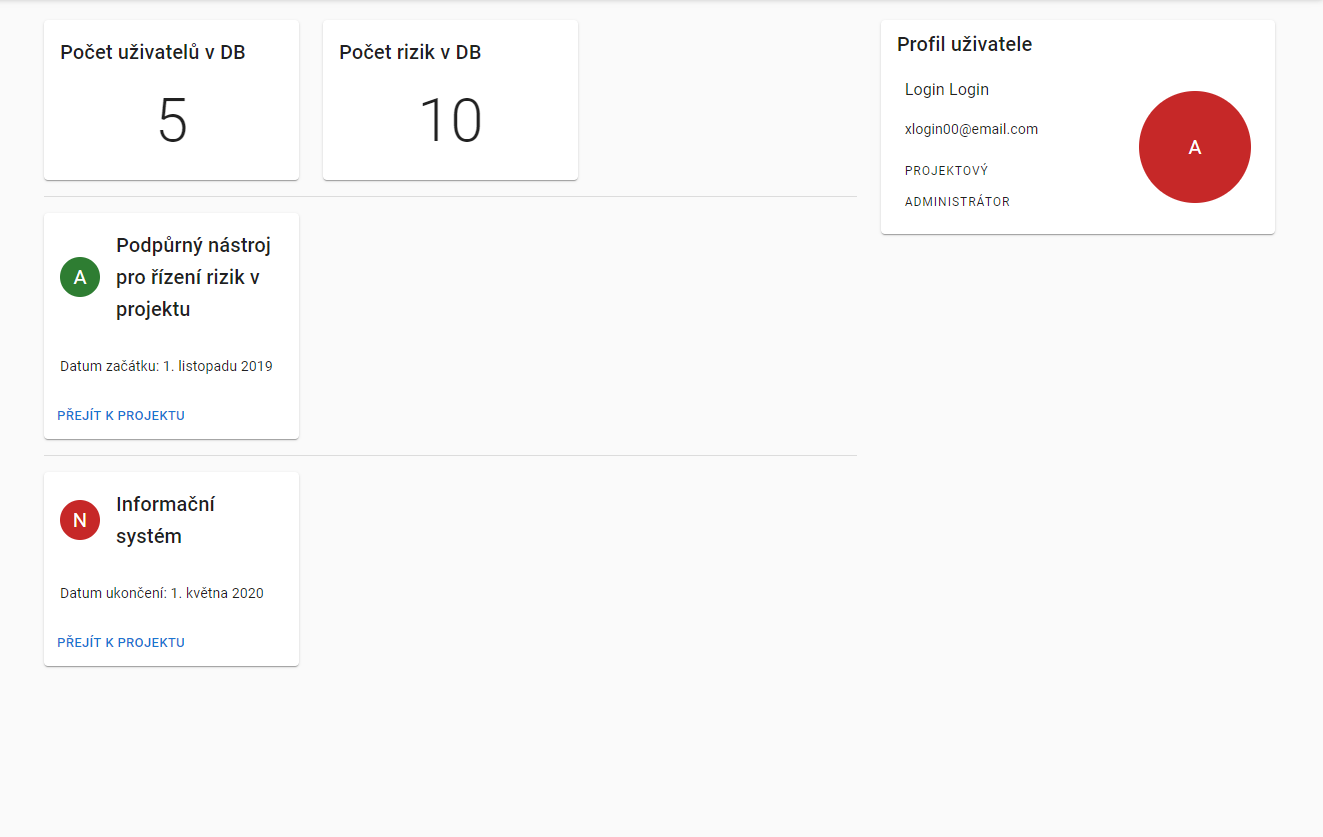
\includegraphics{obrazky-figures/dashboard.png}}
    \caption{Dashboard v~aplikaci pro administrátora [zdroj vlastní]}
    \label{dashboardObrazek}
    \end{center}
    \end{figure}


\subsubsection *{Správa uživatelů}

Správa uživatelů je přístupná pouze administrátorovi a lze ji nalézt na stránce \textbf{/app/users}. Soubory správy uživatelů se nacházejí ve složce user. Hlavní rodičovskou komponentou je zde \texttt{UserTabs}, která následně zobrazuje \texttt{RoleTable}, \texttt{UserBarChart} a \texttt{UsersTable}. 

\texttt{RoleTable} zobrazuje data uživatelských rolí v~tabulce. Klient získá ze serveru id role, její název a id bezpečnostní role. Následně ještě musí komponenta načít id a název bezpečnostních rolí. Výsledná data se zobrazí jako záznamy v~tabulce Role jejíž sloupce jsou název role a název bezpečnostní role. Jako dialog pro přidání a editaci záznamu se používá \texttt{RoleDialog}.

\texttt{UsersTable} funguje na stejném principu jako \texttt{RoleTable}. Komponenta pomocí GET metody získá data všech uživatelů – id, jméno a příjmení, login, heslo, e-mail a id role. Následně se ještě musí získat data rolí, aby bylo možné vytvořit jejich seznam. Dialogem pro tuto tabulku je \texttt{UserDialog}.

\texttt{UserBarChart} je sloupcový graf vytvořený pomocí knihovny Nivo. Zobrazuje kolik uživatelů má přidělenou danou roli. Všechny grafy nacházející se v~aplikaci zobrazují pouze hodnoty, které mají nějaké hodnoty. Pokud tedy danou roli nebude mít přiřazený žádný uživatel, tak se v~grafu nezobrazí.

Komponenty často zobrazují nějaký společný údaj. V~tomto případě všechny tři sdílejí data k~rolím v~systému. Pokud se tedy údaje role změní např. se přiřadí nový uživatel nebo se změní její název, tak musí všechny další komponenty znovu načít data. Informace o~změně se ukládá do Redux store, a všechny komponenty, které můžou být změnou ovlivněné, tak daný údaj sledují a reagují na jeho změnu.


\subsubsection *{Správa projektů}

Nejdůležitější části vytvořeného nástroje je správa projektů. Komponenty, které tvoří tuto část se nacházejí v~adresáři project. Správa projektu se pak dělí ještě na tři další části – zobrazení karet všech projektů, vytvoření a uložení projektu do databáze a potom následuje samotná správa informací na projektu, jeho rizik, swot tabulky a vyplňování dotazníku k~projektu.

Zobrazení všech projektů se nachází na adrese \textbf{/app/project}. Hlavní komponentou je \texttt{ProjectCards}, pomocí které se zobrazují karty s~informacemi ke každému projektu. Na kartě se nachází název projektu, jméno a příjmení vedoucího člena, jeho popis, označení, zda je aktivní nebo ukončený a tlačítka pro smazání a zobrazení podrobných informací o~projektu. Tlačítko na smazání je zobrazitelné pouze administrátorovi, který případné smazání musí ještě odsouhlasit ve výzvě, která se mu zobrazí ve dialogovém okně. Až po tomto odsouhlasení se smažou veškerá projektová data – samotný projekt, záznamy o~přiřazení uživatelů, přidělená rizika, přiřazení dotazníku a statistiky, jak se na něho odpovídalo. Uživateli USER se zobrazí pouze karty projektů, ke kterým je přihlášen (a na rozdíl od dashboardu zde se zobrazí i neaktivní projekty). MANAGER může vidět a zobrazovat všechny projekty. 

\texttt{ProjectCards} také obsahují pole po vyhledávaní zadaného textu v~kartách projektu. Na rozdíl od tabulek, kde tuto funkčnost automaticky poskytuje knihovna material-table, tak v~případě tohoto pole se jeho tvorba inspirovala vzhledem políčka v~tabulkách, jeho funkčnost pak obstarává  funkce \texttt{handleSearchField} v~\texttt{ProjectCards.js}.

\begin{lstlisting}[caption={Části validačního schématu formuláře pro tvorbu projektu},captionpos=b,frame=single,label=validaceSchema]
const validNazevPopis = Yup.object({
    nazev: Yup.string().required('Vyzadovano'),
    popis: Yup.string().required('Vyzadovano'),
});

const validDatumy = Yup.object( {
    start: Yup.date().typeError("Nespravny format datumu: DD. MM. RRRR"),
    konec: Yup.date().typeError("Nespravny format datumu: DD. MM. RRRR")
        .min(Yup.ref('start'), "Datum ukonceni nemuze byt driven 
            nez datum zacatku"),
});

const validManager = Yup.object( {
    manager: Yup.number().typeError("Manazer musi byt zadan")
        .required("Manazer musi byt zadan"),
});

const validationSchemaAll = Yup.object({
    nazev: Yup.string().required('Vyzadovano'),
    popis: Yup.string().required('Vyzadovano'),
    start: Yup.date().typeError("Nespravny format datumu: DD. MM. RRRR"),
    konec: Yup.date().typeError("Nespravny formatdatumu: DD. MM. RRRR")
        .min(Yup.ref('start'), "Datum ukonceni nemuze byt driven 
            nez datum zacatku"),
    manager: Yup.number().typeError("Manazer musi byt zadan")
        .required("Manazer musi byt zadan"),
});

const validationSchema = [validNazevPopis, validDatumy, validManager, 
validationSchemaAll, validationSchemaAll];
\end{lstlisting}

K~vytvoření projektu se lze dostat dvojím způsobem – přejít na adresu \textbf{/app/project/addForm}, která je přístupná pouze administrátorovi nebo při zobrazení karet všech projektu, kliknout na ikonku přidání nového záznamu, který se nachází napravo od vyhledávacího pole (toto tlačítko je opět viditelné pouze administrátorovi).  Jedná se o~několika krokový formulář, který je vytvořen v~komponentě \texttt{AddProjectForm} v~adresáři addProject. Podobně jako ve všech formulářích i tady zodpovídá za jeho správu knihovna Formik, která z~jednotlivých polí získává data a pomocí knihovny yup je validuje. Tento formulář je ale rozdílný tím, že každým krokem se mění jeho validační schéma. Všechny části schématu lze vidět na ukázce kódu \ref{validaceSchema}. Ve formuláři jsou následující části – název a popis projektu, datum začátku a datum předpokládaného konce, přiřazení manažera, přiřazení řešitelů. Formik nedovolí přejít k~dalšímu kroku, pokud validační schéma označuje, že se vyskytuje chyba. Přiřazení řešitelů je jako jediná nepovinná položka. Po odeslání dat na server bude uživatel přesměrován na stránku s~údaji právě vytvořeného projektu, kde může provádět jeho celkovou správu.

Samotná správa projektů se pak nachází na adrese \textbf{/app/project/id}, kde id je id projektu, které mu přidělil server. Je rozdělena na čtyři části – \textbf{základní údaje}, \textbf{rizika}, \textbf{swot} a \textbf{dotazník}. Hlavní komponentou je \texttt{ProjectPageID}, která načte všechna data projektu a uloží je do Redux store. Části pak již načítají potřebná data ze store. Manažeři, kteří nejsou k~projektu přiřazeni si mohou prohlížet jeho údaje, ale nemůžou nic měnit.

\texttt{ProjectInfoTab} zobrazuje komponenty, které se používají pro správu základních údajů projektu (obrázek \ref{projinfo}). Většina se nachází v~adresáři projectInfo. Tlačítko pro editaci údajů jako název, popis a datumy se zobrazí pouze přiřazeným členům řešitelského týmu. Přiřazovat a odhlašovat řešitelé může pouze manažer projektu a manažera pak může změnit pouze administrátor, který zároveň může editovat i všechny předcházející prvky. Pro základní údaje se ve skutečnosti používají dvě komponenty, jedna pro obyčejné zobrazování textu (většinou se jedná o~\texttt{Typography} z~Material-UI) a druhá pro editaci. Tyto komponenty po potvrzení editace údaje, použijí stažená projektová data ze store a odešlou na server novou verzi projektu. Následně se ještě upraví i data v~Redux store. Dodatečně se zobrazují i doplňkové informace o~velikosti řešitelského týmu, zda je projekt stále aktivní, o~počtu přiřazených rizik a kolik dnů zbývá do ukončení projektu.

    \begin{figure}[ht]
    \begin{center}
    \scalebox{0.3}{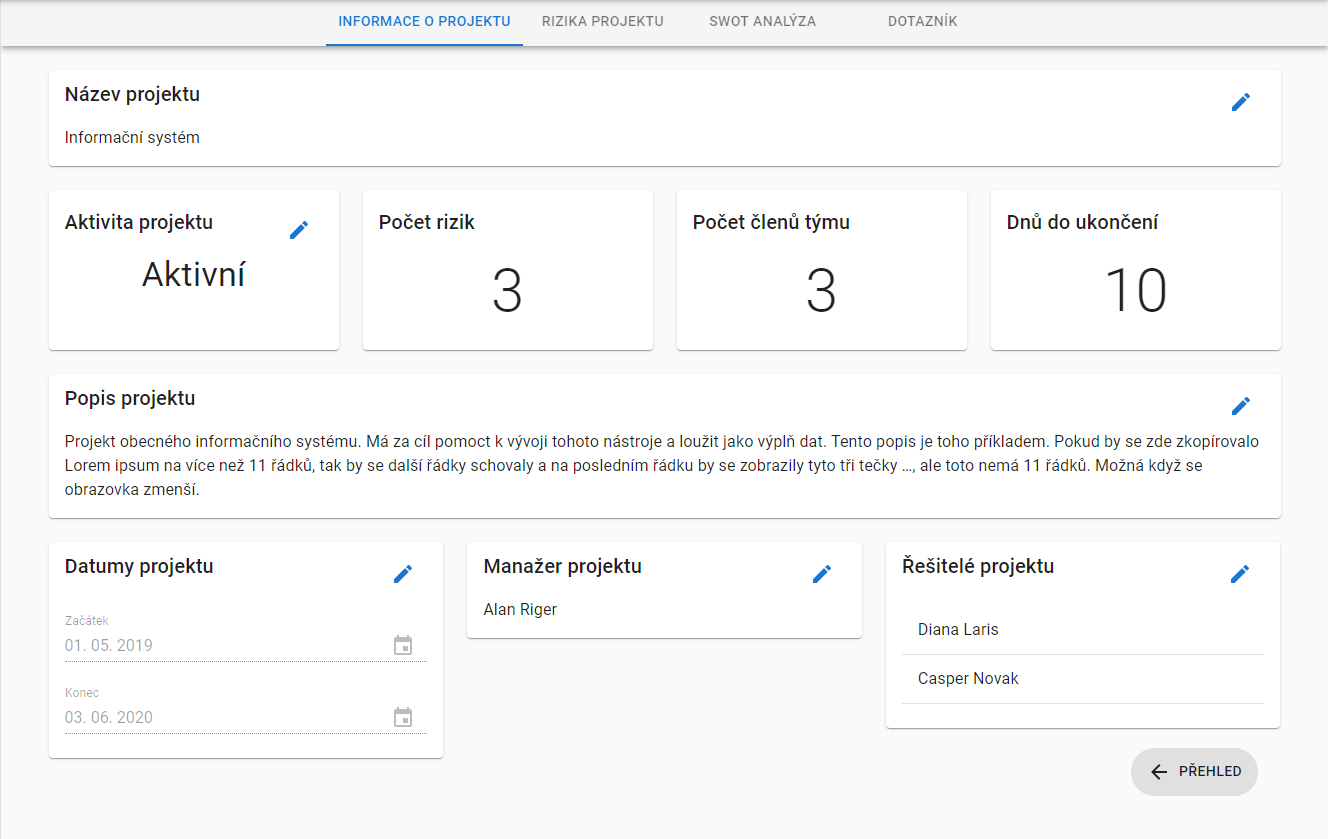
\includegraphics{obrazky-figures/projInfo.png}}
    \caption{Správa základních údajů projektu [zdroj vlastní]}
    \label{projinfo}
    \end{center}
    \end{figure}
    
    
\texttt{ProjectSwotTab} umožňuje správu a zobrazovaní swot tabulky. Komponenta, kterou lze vidět na obrázku \ref{swotinfo} se nachází v~adresáři projectSWOT. V~případě, že projekt nemá swot vytvořené, tak je o~tom uživatel informován a po stisku tlačítka pro tvorbu je mu zobrazena kostra tabulek v~editačním módu. Při pokusu o~smazání dat tabulky, musí akci uživatel ještě potvrdit v~dialogu. Základní komponentou každé položky je \texttt{TextFieldEdit}, která vnitřně používá \texttt{Typography} pro zobrazení a \texttt{InputBase} při editaci. Obě jsou součástí knihovny uživatelských prvků Material-UI. Podobně jako u~správy základních údajů i tady můžou provádět akce spojené s~tabulkou pouze administrátor a uživatelé přiřazení k~projektu.

    \begin{figure}[ht]
    \begin{center}
    \scalebox{0.3}{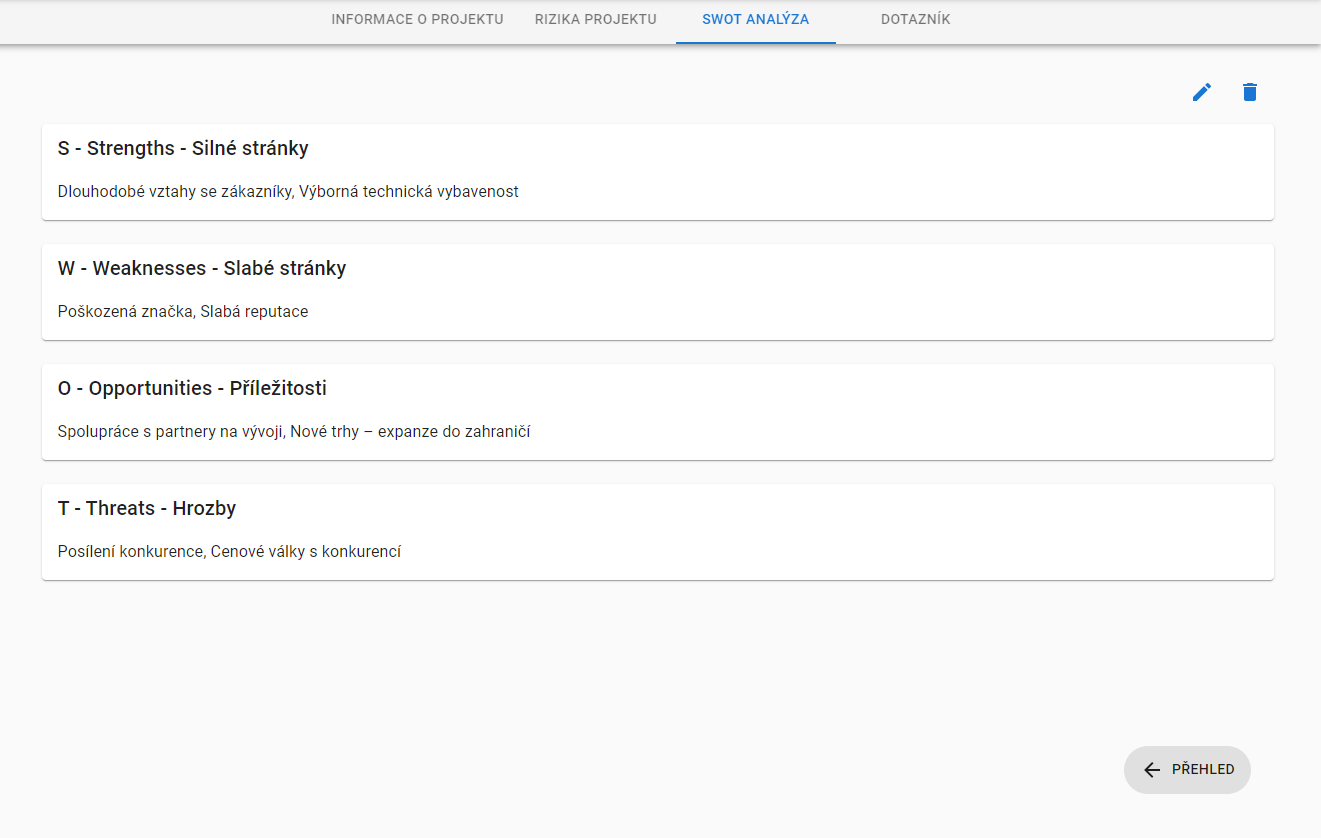
\includegraphics{obrazky-figures/swotinfo.png}}
    \caption{Správa swot tabulky projektu [zdroj vlastní]}
    \label{swotinfo}
    \end{center}
    \end{figure}
    
\texttt{ProjectSurveyTab} je hlavní dotazníkovou komponentou projektu. Společně se svými podpůrnými komponentami se nachází v~adresáři projectSurvey. Podobně jako u~swot tabulky i tady pokud ke projektu není přiřazen žádný dotazník, tak je o~tom, uživatel informován. Tlačítko pro přiřazení je ovšem dostupné pouze manažerovi projektu a administrátorovi. Výběr dotazníků se provádí v~dialogu, který lze vidět na obrázku \ref{addDotaznik}.

    \begin{figure}[!htbp]
    \begin{center}
    \scalebox{0.3}{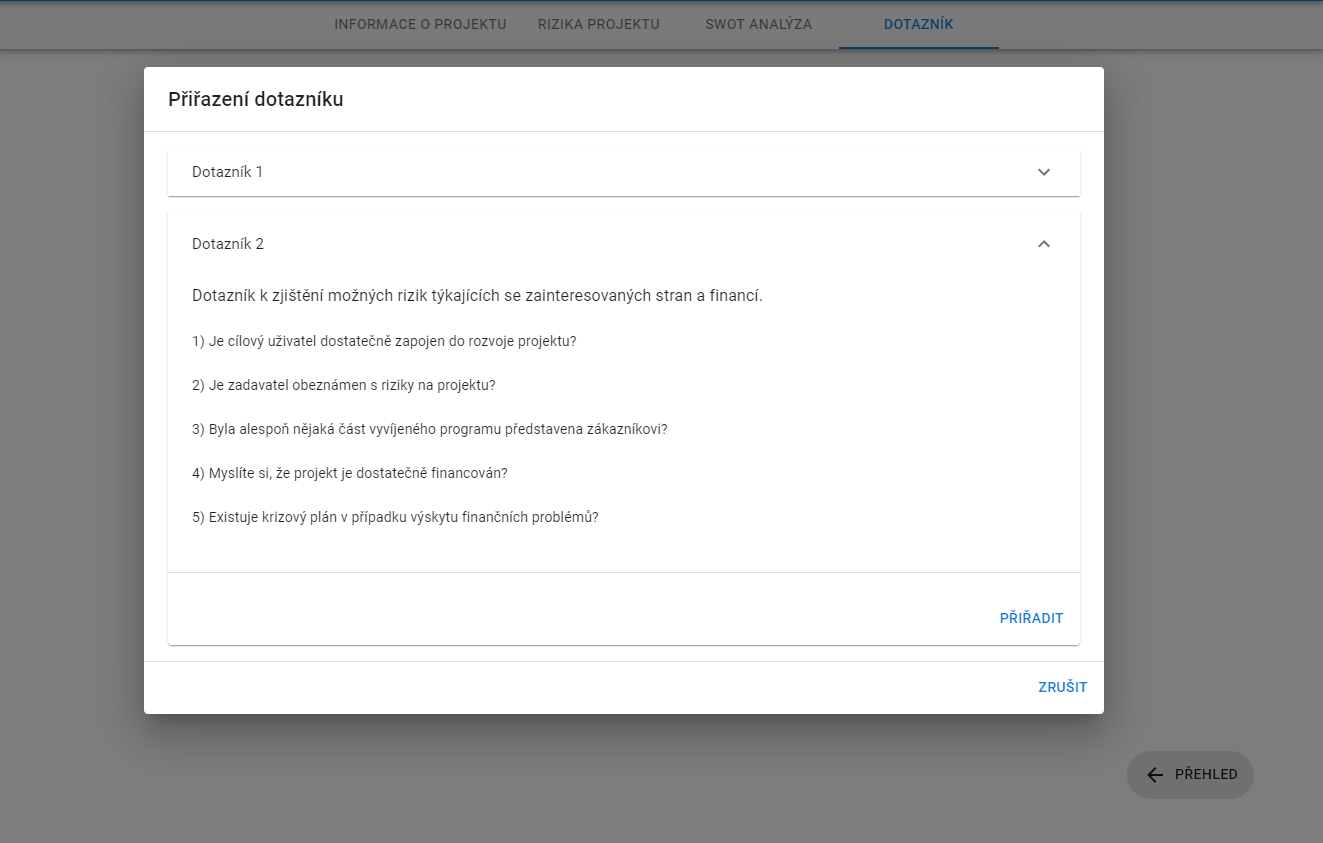
\includegraphics{obrazky-figures/addDotaznik.png}}
    \caption{Výběr dotazníku [zdroj vlastní]}
    \label{addDotaznik}
    \end{center}
    \end{figure}
    
Uživatelovi se v~něm vždy zobrazí jméno dotazníku, jeho popis a jaké obsahuje otázky. Pokud projekt již má přiřazený dotazník, tak se opět zobrazuje jeho jméno, popis a dále také kolik otázek obsahuje a zda již uživatel na dotazník odpověděl. Dále stránka umožňuje dotazník zodpovědět a zobrazit statistiku odpovědí. Řešitelé projektu musí nejprve dotazník zodpovědět, až po tom jim je umožněno statistiku zobrazit. Manažer projektu a~administrátor ji můžou zobrazovat ještě před zodpovězením dotazníku. Statistika se zobrazuje jako procentní hodnocení\,–-\,jaké procento uživatelů (z~celkového počtu co dotazník již zodpovědělo) odpovědělo na danou otázku touto odpovědí. Výsledná hodnota je zaokrouhlena na dvě desetinná čísla a nejvíce používaná odpověď je tučně zvýrazněná. Procenta pro každou odpověď počítá funkce \texttt{countPersentage} z~\texttt{ProjectSurveyTab}.
    
\texttt{ProjectRiskTab} zobrazuje komponenty, které se používají při znázorňování rizik identifikovaných na projektu a které se nacházejí v~adresáři projectRisks. Stránka je rozdělena na čtyři části. První pouze zobrazuje počet přidělených rizik. Druhá pak tvoří skupinu statistických grafů – druhy kategorií přidělených rizik a počet rizik v~daných kategoriích (jedná se o~sloupcový graf), dále pak koláčové grafy znázorňující stav zpracování rizika, pravděpodobnost výskytu, míru dopadů a prioritu při zpracovávaní. Následující tabulka (\ref{tableMaps}) ukazuje mapování slovních popisů atributů rizika používaných v~klientské části s~číselnými hodnotami, které se ukládají do databáze (toto mapování lze také vidět v~definici konstantních proměnných v~adresáři constants).

\begin{table}[h]
\begin{tabular}{|c|c|c|c|c|c|}
\hline
                 & \multicolumn{5}{c|}{\textbf{Hodnota v~databázi}}             \\ \hline
\textbf{Atribut} & 1           & 2            & 3       & 4      & 5            \\ \hline
Stav             & Nové        & Rozpracováno & Hotovo  &        &              \\ \hline
Pravděpodobnost  & Velmi nízká & Nízká        & Střední & Vysoká & Velmi vysoká \\ \hline
Dopad            & Velmi malý  & Malý         & Střední & Vysoký & Velmi vysoký \\ \hline
Priorita         & Malá        & Střední      & Vysoká  &        &              \\ \hline
\end{tabular}
\caption{Mapování slovních popisů klienta na číselné hodnoty z~databáze}
\label{tableMaps}
\end{table}

Poslední dvě komponenty pak tvoří základ správy rizik na projektu. Jedná se o~matici pravděpodobností a dopadů a tabulku s~přidělenými riziky. Základem matice je modifikovaný \texttt{HeatMap} graf z~Nivo knihovny.

    \begin{figure}[!h]
    \begin{center}
    \scalebox{0.45}{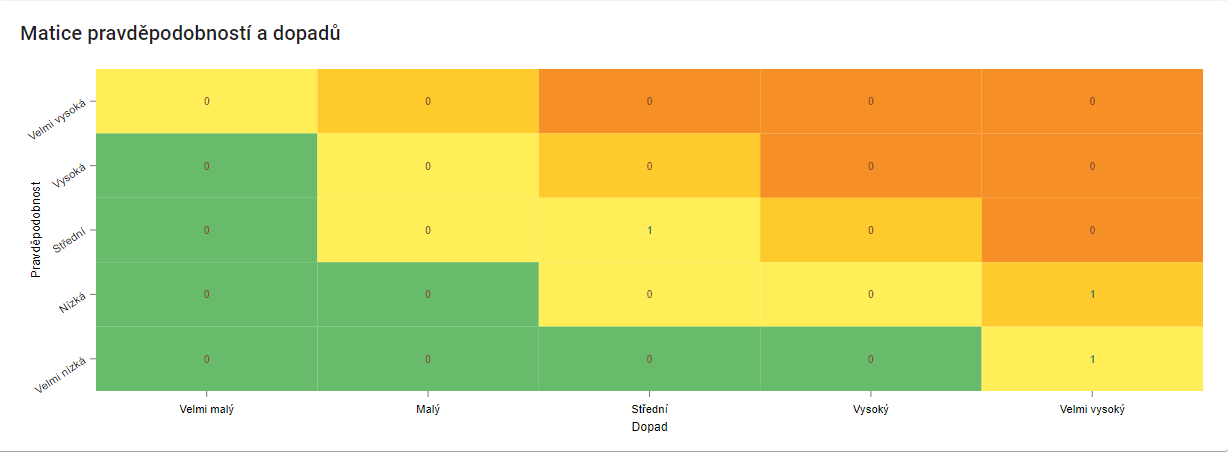
\includegraphics{obrazky-figures/maticePravdDopad.png}}
    \caption{Matice pravděpodobností a dopadů projektu [zdroj vlastní]}
    \label{maticePravdDopad}
    \end{center}
    \end{figure}

Tento graf původně zobrazuje barvu políčka podle toho, jak veliká je hodnota v~dané buňce. Nivo ve výchozím nastavení nabízí dva tvary – čtverec a kruh, umožňuje ale také vytvořit si vlastní tvar. Tento vlastní objekt, v~programu pojmenovaný jako \texttt{MyShape}\footnote{Je vhodné ještě zmínit, že vytvořený objekt MyShape je převzatý z~knihovny Nivo a ve výchozím nastavení se používá pro zobrazení čtvercového tvaru, dodatečně se v~něm ale ještě jednou vypočítává barva, kterou se má vykreslit.}, dostane již od Nivo přidělenou barvu (jak již bylo řečeno, podle hodnoty políčka), je možné ale ještě dodatečně vypočítat novou barvu a tou nahradit původně přidělenou. Barvu políčka vypočítává funkce \texttt{calculateColor}, která využívá vynásobenou číselnou hodnotu pravděpodobnosti a dopadu. Komponenta matice se nazývá \texttt{RiskMatrix}. Ve svých buňkách ukazuje počet rizik, které v~atributech mají danou kombinaci hodnoty pravděpodobnosti a~dopadu. Při najetí myši dané políčko, se zobrazí názvy rizik, které se tam nacházejí. Matici pravděpodobností a dopadů lze vidět na obrázku \ref{maticePravdDopad}.

    
Poslední komponentou je tedy tabulka rizik přiřazených k~projektu. Lze ji vidět na obrázku \ref{registrRizikTable} a tvoří ji hlavně komponenta \texttt{ProjectRiskTable}. Tato tabulka se mírně liší od ostatních tím, že je možné jednotlivé záznamy rozkliknout a nechat si tak zobrazit podrobnosti.

    \begin{figure}[!h]
    \begin{center}
    \scalebox{0.45}{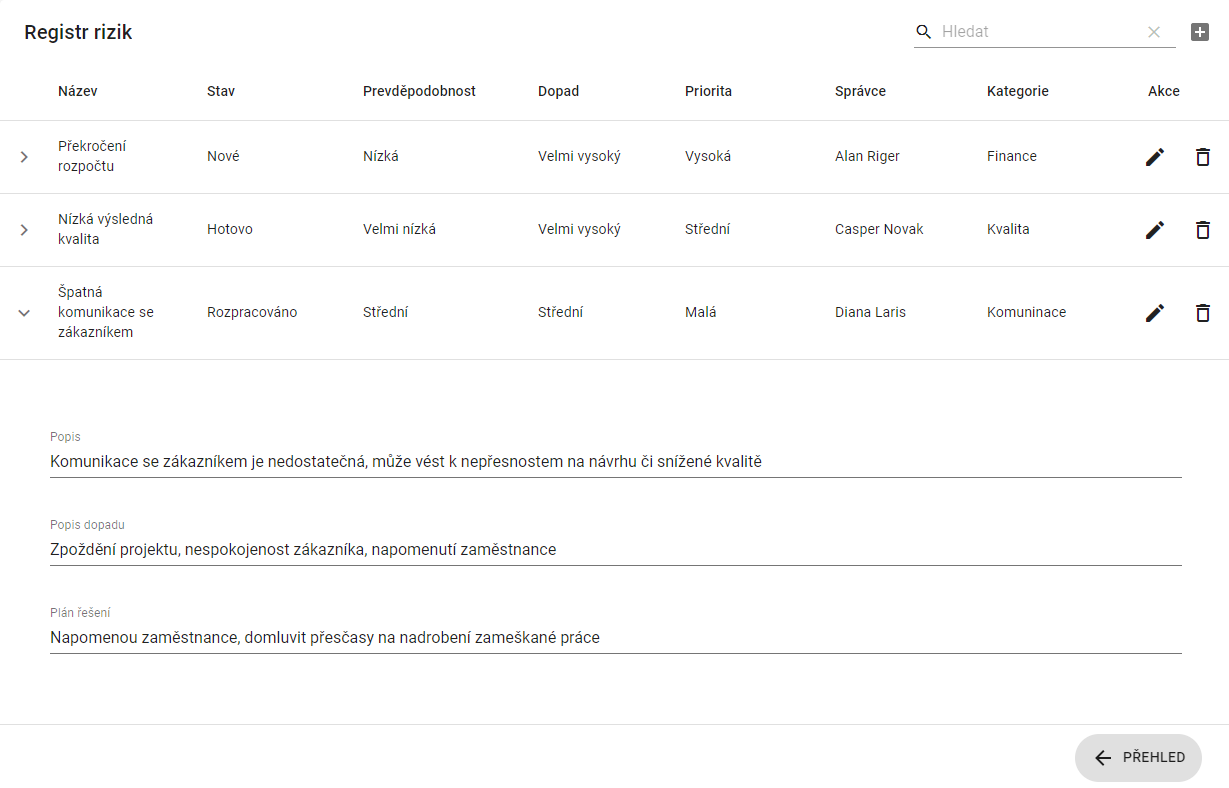
\includegraphics{obrazky-figures/registrRizik.png}}
    \caption{Registr rizik projektu s~otevřeným zobrazením podrobností u~prvního rizika [zdroj vlastní]}
    \label{registrRizikTable}
    \end{center}
    \end{figure}

Tato tabulka se mírně liší od ostatních tím, že je možné jednotlivé záznamy rozkliknout a nechat si tak zobrazit podrobnosti. Přidat riziko k~projektu lze dvěma způsoby, buď se vybere již nějaké vytvořené z~centrálního registru rizik nebo se vytvoří nové, které se při ukládání na server automaticky uloží i do centrálního registru. V~případě, že uživatel se pokusí přiřadit riziko, které se již v~tabulce nachází, tak na to bude upozorněn a pokud ho i tak uloží, tak nově uložené hodnoty přepíšou ty původní.


\subsubsection *{Centrální registr rizik}

Registr rizik je dostupný všem uživatelům a zobrazuje se na adrese \textbf{/app/register}. Komponenty se nacházejí v~adresáři riskRegister, přičemž \texttt{MainRiskRegisterPage} pak po stránce rozmísťuje následující čtyři komponenty. 

\texttt{RiskCategoryTable} a \texttt{RiskRegisterTable} jsou funkčností a vzhledem obdobné s~tabulkami ve správě uživatelů. První slouží pro tvorbu, editaci a smazání možných kategorií rizik. Druhá tabulka pak představuje centrální registr rizik, ze kterého se k~projektům přidělují rizika. Každá z~nich používá odpovídající dialog pro tvorbu a editaci záznamů

\texttt{CategoryBarChar} a \texttt{RiskInProjectChart} jsou dodatečné statistické sloupcové grafy. První zobrazuje graf Kategorie rizik, kde se ukazuje počet rizik v~jednotlivých kategoriích. Z~grafu \texttt{RiskInProjectChart} lze pak vyčíst kolikrát se dané riziko již k~nějakému projektu přiřadilo.



\subsubsection *{Správa dotazníků}

Rozdělení správy dotazníků je podobné správě projektů. Také se jedná o~tři části – zobrazení shrnujících karet, přidávání a editace dotazníků. Opět se jedná o~část nástroje, ke které má přístup pouze administrátor. Komponenty používané v~dotaznících se většinou nacházejí v~adresáři survey.

Zobrazení karet dotazníků provádí \texttt{MainSurveyPage} a jeho podpůrná komponenta \texttt{Sur\-veyCards}. Lze k~nim přistoupit na adrese \textbf{/app/survey}. Na kartách se zobrazuje název dotazníku, jaký počet otázek obsahuje a zda je přiřazen k~nějakému projektu. Dále také obsahují odkaz na přesměrování na stránku s~podrobnými daty dotazníku a tlačítko na jeho smazání. Na stránce \texttt{MainSurveyPage} se nachází i tlačítko na vytvoření dotazníku.

Podrobné údaje dotazníku lze zobrazit na stránce \textbf{/app/survey/id}, kde id je id dotazníku, které mu přidělil server. Hlavními komponentami jsou \texttt{SurveyInfoPage} a \texttt{SurveyInfo} z~podadresáře surveyInfo. Na této stránce může administrátor editovat název, popis, přidávat a odebírat otázky. Výběr otázky probíhá pomoci dialogu, kde lze filtrovat otázky podle oblastí.

Tvorba dotazníku probíhá na adrese \textbf{/app/survey/addSurvey} a využívá stejné komponenty, které se používají při editaci dotazníku. 


\subsubsection *{Správa otázek a odpovědí}

Stránka správy otázek a odpovědí, která se nachází na adrese \textbf{/app/question}, je tvořena třemi tabulkami, které umožňují zobrazování a správu odpovědí, oblastí otázek a samotných otázek. Hlavní komponentou, která zobrazuje již zmíněné tři části je \texttt{MainQA} nacházející se v~adresáři questionAnswer. Stránka je přístupná pouze administrátorovi. 

Tabulky Odpovědi (\texttt{AnswersTable}) a Oblasti otázek (\texttt{QuestionAreaTable}) fungují na stejném principu jako již předem představené tabulky např. tabulka Role ve správě uživatelů či tabulka Kategorie v~centrálním registru rizik.

Tabulka Otázky (\texttt{QuestionTable}) umožňuje u~jednotlivých záznamů si nechat zobrazit jaké obsahují odpovědi. Při tvorbě otázky lze dynamicky přidávat a odebírat přiřazené odpovědi, vždy ale musí být minimálně dvě a nesmí se opakovat.


\subsubsection *{Zobrazení chyb}

Nástroj umožňuje zobrazovat několik druhů chyb. První druh se zobrazuje při vyplňování formulářů, které jsou spravovány pomocí knihovny Formik a validace probíhá pomocí Yup. Pokud zadaná hodnota nesplňuje validační schéma (nebo je hodnota povinná, ale uživatel nic nezadal), tak Formik, k~danému políčku propaguje chybu. Vstupní prvky Material-UI mají výchozí podporu zobrazování chyb, kdy se políčko zabarví do červené a pod něj se vypíše chybová zpráva. Příklad lze vidět na obrázku \ref{fromikErr}, kdy uživatel při tvorbě projektu zadal datum ukončení před datumem začátku projektu.

    \begin{figure}[!h]
    \begin{center}
    \scalebox{0.45}{
\includegraphics{obrazky-figures/fromikError.png}}
    \caption{Indikace chyby při vyplňování formuláře [zdroj vlastní]}
    \label{fromikErr}
    \end{center}
    \end{figure}
    
Druhým druhem chyb jsou chybové stavy, které se vrátí ze serveru. Jedná se hlavně o~chybové kódy \textbf{401 Neautentizováno} a \textbf{404 Nenalezeno}. Neautentizováno se vrátí v~případě, že server z~nějakého důvodu odhlásí uživatele, velmi často z~důvodu neaktivity. Nenalezeno vrátí, pokud uživatel chce získat zdroj, který neexistuje, v~případě tohoto nástroje se může jednat o~pokus o~zobrazení neexistujícího projektu či dotazníků. Pro tento druh chyb je vytvořena komponenta \texttt{MyErrorHandler}, adresář error, která \uv{obaluje} celou aplikaci (aplikace je tedy jejím potomkem). Komponenta sleduje \textbf{error} stav v~Redux store, který se nastaví na chybový kód, pokud některý axios požadavek se vrátí jako neúspěšný s~daným chybovým stavem. V~případě, že je \textbf{error} stav nastaven, tak se zobrazí odpovídající chybová stránka. Při 401 se uživateli vysvětlí, že byl serverem odhlášen a je mu zpřístupněn odkaz na přihlašovací stránku. Při 404 se pak na chybové stránce nachází odkaz na dashboard uživatele. Pokud ale error stav nastavený nebude, tak \texttt{MyErrorHandler} zobrazí svého potomka přesněji aktuální komponentu aplikace.


\subsubsection *{Tmavý vzhled}

Pokud uživatel preferuje tmavý vzhled aplikace, tak hlavní panel aplikace obsahuje tlačítko pro přepnutí do tmavého režimu. Material-UI definuje styl jednotlivých prvků pomocí tzv. \textit{theme} a pokud chce vývojář tento objekt modifikovat a změny propagovat dále do aplikace, tak musí použít komponentu \texttt{ThemeProvider} z~knihovny Material-UI, kterou „obalí“ aplikaci. Theme je ve výchozí konfiguraci nastavena na světlou verzi stylu, ale velice jednoduše lze přepnout do tmavé verze a to přiřazením řetězce \texttt{dark} do proměnné \texttt{palette.type}. Tato modifikace způsobí automatickou změnu několika dalších proměnných, které se týkají barev používaných v~aplikaci. Jako indikace právě používaného módu se používá proměnná \texttt{appTheme} v~Redux store.

\chapter{Testování}
\label{testovani}

Testování softwaru se provádí vždy za účelem něco zjisti. Ať už se jedná o~zjištění kvality vytvořeného nástroje nebo ověření stavu databáze po provedení určité akce. Testy lze také automatizovat, kdy se spustí celé sady testů jejichž výsledek lze předpovědět. Výsledky těchto testů se pak porovnávají se předpovězenými hodnotami a tím se určí jejich úspěch či neúspěch.  

V~této kapitole se popisuje průběh a způsob testování nástroje. Je rozdělena na tři části, kde v~první se popisují automatizované testy prováděné na serveru. Ve druhé se krátce popíše práce s~programem Postman a laděním API serveru. Třetí část pak popisuje testovací scénáře použití při uživatelském testování klienta. 


\section{Automatizované testování}

Spring Boot umožňuje vytvářet automatizované testy a podobně jako při programování jednotlivých modulů i zde lze testy vytvářet různými způsoby. Zároveň lze také vytvářet oddělené testy pro jednotlivé části aplikace. 

Automatizované testy byly vytvořené pro serverovou část jako integrační testy, které mají určit, zda nově přidané moduly správně spolupracují s~ostatními a netvoří neočekávané chyby. Testy se tvořily již v~průběhu programování jednotlivých částí serveru, kdy nejprve se vytvořil test a následně se doprogramovaly jednotlivé potřebné moduly. Spojují části service, repository a domain. Soubory s~testovacími metodami se nacházejí adresáři test, kde každá metoda je anotovaná s~\texttt{@Test}. Každý test je samostatnou jednotkou a neovlivňuje další testy, což znamená, že ačkoliv test může změnit databázi, tak po jeho ukončení jsou všechny změny vráceny zpět. V~rámci této sekce testování se vytvořilo 70 integračních testů.


\section{Postman a API}

Program Postman se využíval při tvorbě řadičů (\textit{controller}), které umožňují reakci na volání API serveru. V~Postman lze vytvářet jednotlivé REST požadavky a zasílat je na server. Funguje tedy jako náhrada za klientskou část pro otestování a ladění reakcí na požadavky. 

Při tvorbě požadavku lze ovlivňovat celý jeho formát – cookies co se mají poslat, hlavičky, jaká data a v~jakém formátů. Po jeho odeslání Postman přijme ze serveru odpověď, ve které lze např. zkoumat její status, přeposlaná data, cookies, hlavičky atd. V~případě, že požadavek byl chybný, tak se zobrazí odpovídající chybová zpráva i se svým kódem, kterou server poslal zpět.

Postman umožňuje také vytvářet automatizované testy, které zkoumají a vyhodnocují odpovědi získané ze serveru. Dohromady bylo takto vytvořeno a otestováno 71 REST požadavků.


\section{Uživatelské testování}

Cílem uživatelských testů bylo zjistit použivatelnost výsledného nástroje. Bylo vytvořeno několik testovacích scénářů, které postupně měly provést uživatele přes jednotlivé případy použití. Tyto scénáře nejsou klasickými krokovými testy, kdy je uživatel pozorován, jak jednotlivé kroky plní.  Místo je uživateli popsaná situace (scénář) ve které se nachází, přičemž bude na něm, jak se s~danou situaci vypořádá.

Žádný z~testerů se s~aplikací během jejího vývoje nesetkal, ale z~důvodu aktuální pandemické situace není ani jeden z~nich přímo svázán s~řízením projektů či s~vyhledáváním rizik. Místo toho jsem vybrala testery, kteří mají již trochu rozsáhlejší znalosti práce na počítači nebo jsou v~průběhu studia na univerzitě technického zaměření. Toto by mohlo simulovat malý tým pracující na nějakém start-upu. Všechny testy probíhaly na lokálním stroji, na kterém byl nástroj tvořen. Část testerů byla fyzicky přítomná při notebooku s~aplikaci, druhá část pak ovládala aplikaci vzdáleně pomocí sdílené obrazovky a sdíleném ovládání myši a klávesnice. Ke sdílení se použila aplikace Zoom.

Před začátkem testování bylo každému uživateli vysvětleno k~čemu aplikace slouží, v~jaké situaci se nachází a co má za úkol. Při plnění jednotlivých scénářů, které lze vidět v~následujícím seznamu, byla snaha uživateli téměř nenapovídat.

\begin{enumerate}
    \item Firma přijala dva nové zaměstnance\,--\,Alana Rigera na pozici projektového manažera a Betty Rocky jako členku řešitelského týmu. Je nutní jim vytvořit účet, aby mohli aplikaci využívat. Tuto akci může provádět pouze administrátor.
    \item Firma získala zakázku na nový projekt se zaměřením na záchranu velkých kočkovitých šelem. Jako administrátor je tvou povinností tento projekt vytvořit v~nástroji a tím ho uložit do databáze. Název projektu je Kočkovité šelmy a je popsán jako projekt vytvoření informačního systému pro záchrannou stanici velkých kočkovitých firem. Začátek prací na projektu byl stanoven na 20.5.2020 a konec se předpokládá někdy na druhou polovinu roku 2022. Nově přijatí zaměstnanci (Alan Riger a Betty Rocky) jsou prvními členy řešitelského týmu a jsou přiřazeni ke svým odpovídajícím pozicím.
    \item Pro projekt Kočkovité šelmy je nutné vytvořit nový dotazník, který může pomoct řešitelům projektu identifikovat rizika, která se mohou vyskytnou na tomto projektu. Před tvorbou dotazníku je vhodné zkontrolovat, zda v~nástroji existují požadované otázky, které má dotazník obsahovat.
    \item Jako manažer (Alan Riger) ti byl přiřazen nový projekt, který máš řídit. Projekt má pracovní název Kočkovité šelmy. Nově bylo ustanoveno, že datum ukončení bude 30.9.2022. Zároveň ti bylo sděleno, že Betty Rocky byla přesunuta do jiného projektu a jako náhrada za ní je přidělena Diana Laris. Změn informace na projektu, aby odpovídaly novým skutečnostem.
    \item Řešitelský tým projektu Kočkovité šelmy identifikoval dva nová rizika. Riziko Překročení rozpočtu z~kategorie Finance je již známé a je již uložené v~centrálním registru rizik. Projekt je ale dobře financován, takže i když má střední pravděpodobnost výskytu, tak bude mít na projekt pouze minimální dopad. Druhé riziko tým identifikoval poprvé – Pandemie infekční nemoci. Z~důvodu situace ve světě je veliká pravděpodobnost, že riziko zastihne i tento projekt, přičemž bude mít nejvyšší úroveň dopadu. Z~tohoto důvodu by riziko mělo mít nejvyšší prioritu dalšího řešení. Jelikož se první riziko týká financí je vhodné, aby ho měl na starost manažer projektu. U~druhého rizika může být správcem kdokoliv.
    \item Jako manažer se chystáš vytvořit SWOT analýzu projektu Kočkovité šelmy. Pro jednodušší práci se můžeš inspirovat jinými projekty v~systému.
    \item Bylo ti oznámeno, že dotazník k~projektu Kočkovité šelmy je připraven. Přiřadit ho k~tomuto projektu, aby ostatní řešitelé mohli na něho odpovídat. Tuto akci proveď jako manažer daného projektu.
    \item Jednou z~povinností řádového člena týmu je zodpovědět dotazník, který byl přiřazený k~projektu, na kterém daný člen pracuje. Ujisti se, že jsi na něho zodpověděl a pokud ne, tak ho zodpověz.
    \item Zajímá tě, jak ostatní uživatelé odpověděli na dotazník. Zjisti si tuto informaci.
    \item Jsi ve tmavé místnosti a bílé pozadí aplikace dráždí tvé oči. Pokus se tento problém v~aplikaci vyřešit.
    \item Dostal jsi za úkol přepsat z~papíru několik rizik do centrálního registru\,--\,proveď to.
    \item Projekt kočkovité šelmy skončil neúspěchem. Firma nechce uchovávat jeho data. Jako administrátor jsi dostal za úkol tento projekt ze systému odstranit.
\end{enumerate}


\chapter{Možné rozšíření}
\label{rozsireni}

\chapter{Závěr}
\label{zaver}

Tento semestrální projekt reflektuje aktuální stav vytváření diplomové práce Nástroj pro podporu managementu rizik. Úvodem práce jsem musela nastudovat obecnou problematiku znalostních oblastí řízení projektu. Následně se jsem se pak musela blíže seznámit s~procesy plánování, identifikace a kvalitativní analýzy ze znalostní oblasti řízení rizik. Všechny tyto informace lze nalézt v~kapitole \ref{teorie} a hlavně vycházejí z~nejnovějšího rozsáhlého standardu o~řízení projektu od firmy PMI.  Dále jsem také představila, jak se při agilním řízení projektu nahlíží na jednotlivé znalostní oblasti.

Pomocí získaných znalostí jsem pak specifikovala požadavky na výsledný nástroj. Ten by měl podporovat uživatele při identifikaci a analýze rizik a zároveň by měl umožňovat vizualizaci rizik na projektu. Výsledná aplikace by měla být uživatelský přívětivá s~moderním vzhledem. Tento nástroj jsem následně navrhla jako webovou klient--server aplikaci. 

Na základě osobních preferencí jsem se rozhodla, že k~naprogramovaní serverové části se použije Spring Boot framework. Pro klientskou část se použije javacsriptová knihovna React od firmy Facebook s~dodatečnými knihovnami podle potřeby. Jednou s~dodatečných knihoven bude s~jistotou Material UI, která obsahuje prvky uživatelského rozhraní splňující podmínky Material Design do firmy Google (část o~použitých technologiích již v~této práci zahrnuto není, ale je rozpracováno).

\section{Další vývoj diplomové práce}

V~následujícím semestru pak bude probíhat pokračování psaní textu této práce. Podrobně se představí technologie, které se použijí k~implementaci navrhnutého nástroje. V~případě potřeby se v~tomto textu také popíšou zajímavé či důležité pasáže kódu. Následně se představí vhodné techniky testovaní a vyberou se ty, pomocí kterých bude implementovaný systém testován. Také se zhodnotí použitelnost nástroje v~reálném prostředí. V~závěru práce se pak zhodnotí dosažené výsledky a zmíní se i případné další možnosti rozšíření vytvořeného systému v~budoucnu.

Co se týče praktické části této práce\,--\,vytvoření navrženého nástroje, tak tam se bude pokračovat ve studiu zvolených vývojových prostředku potřebných k~jeho naimplementování. Souběžně také bude probíhat implementace schváleného návrhu a v~případě potřeby také opravy či rozšíření stávajícího návrhu, který byl vytvořen v~rámci semestrálního projektu.





%===============================================================================
